% NOTE:
%" latexmk -shell-escape -pvc slides.tex # Watches and compiles on each change.
% latexmk -c slides.tex   # Clean the temporal files.

% NOTE:
% the minted package doesn't play well with the bibliography!

\documentclass[aspectratio=169]{beamer}

\setbeamertemplate{footline}[frame number]

\usepackage{caption}
\usepackage{graphicx}
\usepackage{hyperref}
%\usepackage{subcaption}
%\captionsetup[figure]{labelformat=empty}

\title{Exploratory analysis of recurrent deforestation warnings in the the
Brazilian Amazon}

\author{Alber Sanchez\\alber.ipia@inpe.br}
\institute{
    
\includegraphics[width=4cm,keepaspectratio]{./logos/trees-color-h_2.png}
    
\includegraphics[width=1.8cm,keepaspectratio]{./logos/logoinpe-azul-menor.png} \\
    TreesLab\\Instituto Nacional de Pesquisas Espaciais - INPE\\Brazil
}
\date{\today}

\begin{document}

\frame{\titlepage}

%\begin{frame}{Outline}
%    \tableofcontents
%\end{frame}

\AtBeginSection[ ]
{
    \begin{frame}{Outline}
        \tableofcontents[currentsection]
    \end{frame}
}

\section{Introduction}


\begin{frame}
    \frametitle{Deforestation}
    \begin{columns}
        \begin{column}{0.5\textwidth}
            It's a conversion by suppression of areas of primary vegetation
            due to anthropogenic actions~\cite{dealmeida2022}.
            \begin{itemize}
                \item Clear-cut deforestation is the complete removal of forest cover in
                    a short period of time~\cite{dealmeida2022}.
                \item Progressive forest degradation. It's the same as clear-cut
                    deforestation, but it takes longer (years).
            \end{itemize}
        \end{column}
        \begin{column}{0.5\textwidth}
            \begin{figure}[h]
                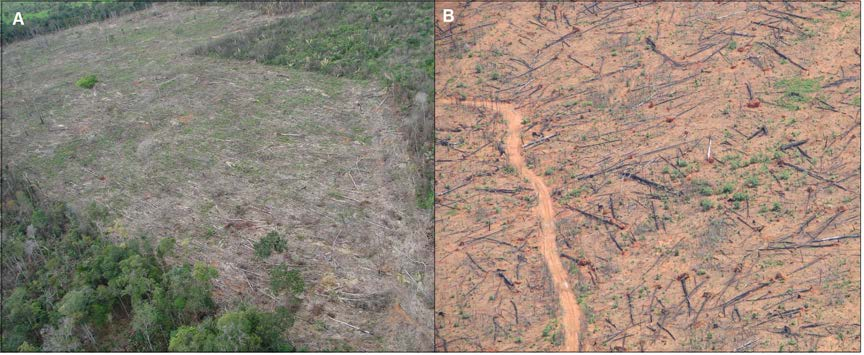
\includegraphics[width=0.99\linewidth]
                {./images/clear_cut_photo.png}
                \caption{Clear-cut deforestation in tow Mato Grosso's towns:
                (A) Tapurah, (B) Santa Carmen. Source~\cite{dealmeida2022}}
            \end{figure}
        \end{column}
    \end{columns}
\end{frame}

\begin{frame}
    \frametitle{Deforestation processes}
    \begin{itemize}
        \item Clear-cut deforestation.
        \item Progressive forest degradation.
    \end{itemize}
\end{frame}

\begin{frame}
    \frametitle{Deforestation due to Progressive Forest Degradation}
    \begin{columns}
        \begin{column}{0.5\textwidth}
            \begin{enumerate}
                \item Removal of trees with the highest value wood, then
                    wood for construction and light wood trees for plywood and
                    boards.
                \item Smaller trees are felled and undergrowth is destroyed.
                    Pasture sowing occurs, and it is burned during the second
                    year (second cleaning). Then cattle is introduced and
                    year more fire destroys the remaining forest (third year).
                \item Complete loss of the canopy, collapse of forest's
                    structure and loss of ecological functions. No more
                    forests' self-regeneration.
            \end{enumerate}
        \end{column}
        \begin{column}{0.5\textwidth}
            \begin{figure}[h] 
                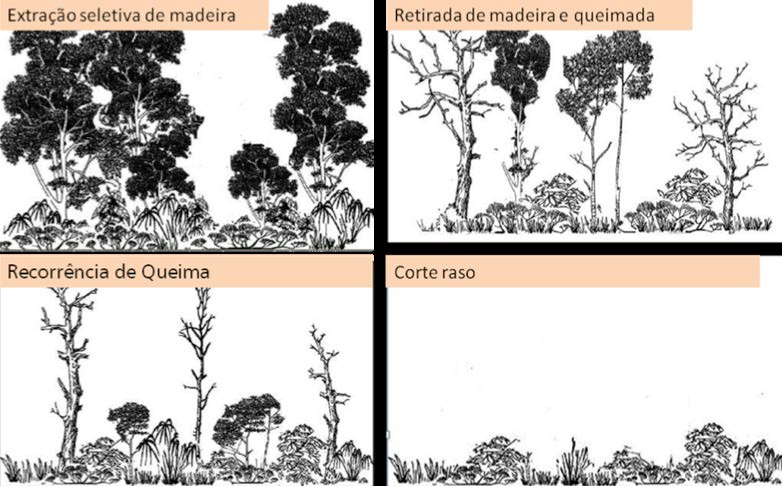
\includegraphics[width=0.9\linewidth]
                {./images/progressive_degradation_drawing.png}
                \caption{Progressive forest degradation. 
                Source~\cite{dealmeida2022}.}
            \end{figure}
        \end{column}
    \end{columns}
\end{frame}

\begin{frame}
    \frametitle{Deforestation due to Progressive Forest Degradation}
    \begin{figure}[h] 
        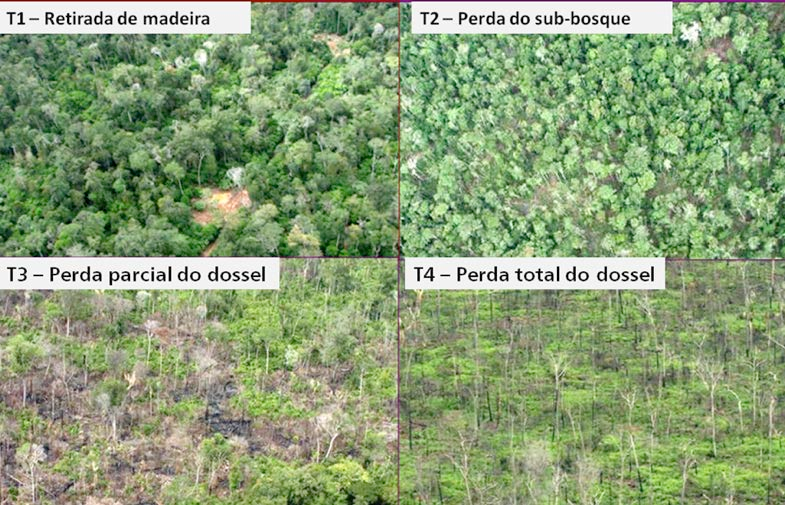
\includegraphics[width=0.72\linewidth]
        {images/progressive_degradation_photo.png}
        \caption{Process of progressive forest degradation.
        Source~\cite{dealmeida2022}.}
    \end{figure}
\end{frame}

\begin{frame}
    \frametitle{Challenges}
    \begin{itemize}
        \item Deforestation by successive degradation remains a challenging 
            question in the scientific literature.
        \item We think a potential answer to this question could be found in 
            DETER's warnings.
        \item This answer could play an important role, for example, for 
            improving the national estimation of greenhouse gases.
    \end{itemize}
\end{frame}

\section{Materials and methods}

% TODO: What is PRODES?

\begin{frame}
    \frametitle{What is DETER?}
    \begin{columns}
        \begin{column}{0.5\textwidth}
            \begin{itemize}
                \item It is a GIS which produces a fast assessment of deforestation 
                    and forest degradation in the Brazilian 
                    Amazon~\cite{shimabukuro2006}.
                \item It employs experts to detect and issue warnings of
                    deforested or degraded areas~\cite{dealmeida2022}.
                    %larger than 3 ha
                \item Annually, DETER takes from PRODES the current forested area, 
                    starting anew issuing warnings.
                \item Data publicly available from 
                    \href{https://terrabrasilis.dpi.inpe.br}{Terrabrasilis}.
            \end{itemize}
        \end{column}
        \begin{column}{0.5\textwidth}
            \begin{figure}[h]
                
\includegraphics[width=0.99\linewidth]{./logos/deterblogo.jpg}
                
\includegraphics[width=0.65\linewidth]{./logos/terrabrasilis.png}
            \end{figure}
        \end{column}
    \end{columns}
\end{frame}


%[1] "Number of DETER subareas:"
%[1] 269832

%[1] "Number of DETER alerts:"
%[1] 328164

%[1] "DETER date range:"
%[1] "2016-08-02" "2021-07-31"



\begin{frame}
    \frametitle{DETER warnings}
    \begin{columns}
        \begin{column}{0.5\textwidth}
            \begin{itemize}
                \item Polygons from 2016 to 2021.
                \item Note that, the spatial properties of DETER warnings are
                    inconsistent along time (shape, size, area, position).
                \item The figure shows 3 DETER warnings from different dates
                    with partial overlap.
            \end{itemize}
        \end{column}
        \begin{column}{0.5\textwidth}
            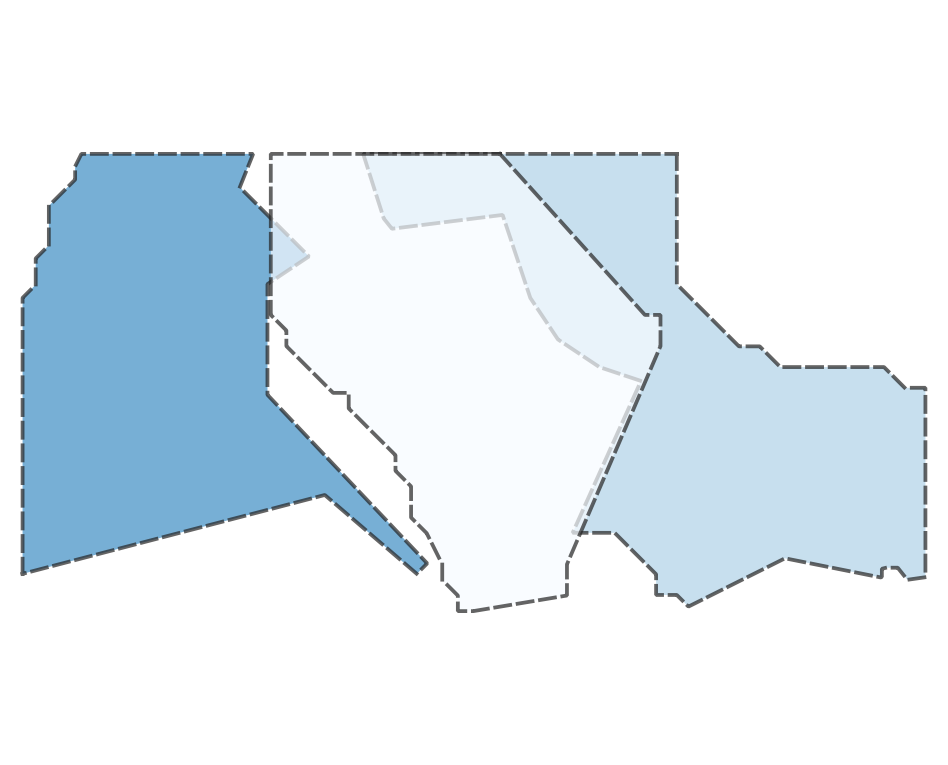
\includegraphics[width=0.99\linewidth]
            {./images/sample_deter_warnings.png}
        \end{column}
    \end{columns}
\end{frame}

\begin{frame}
    \frametitle{Area of DETER warnings}
    \begin{figure}[h]
        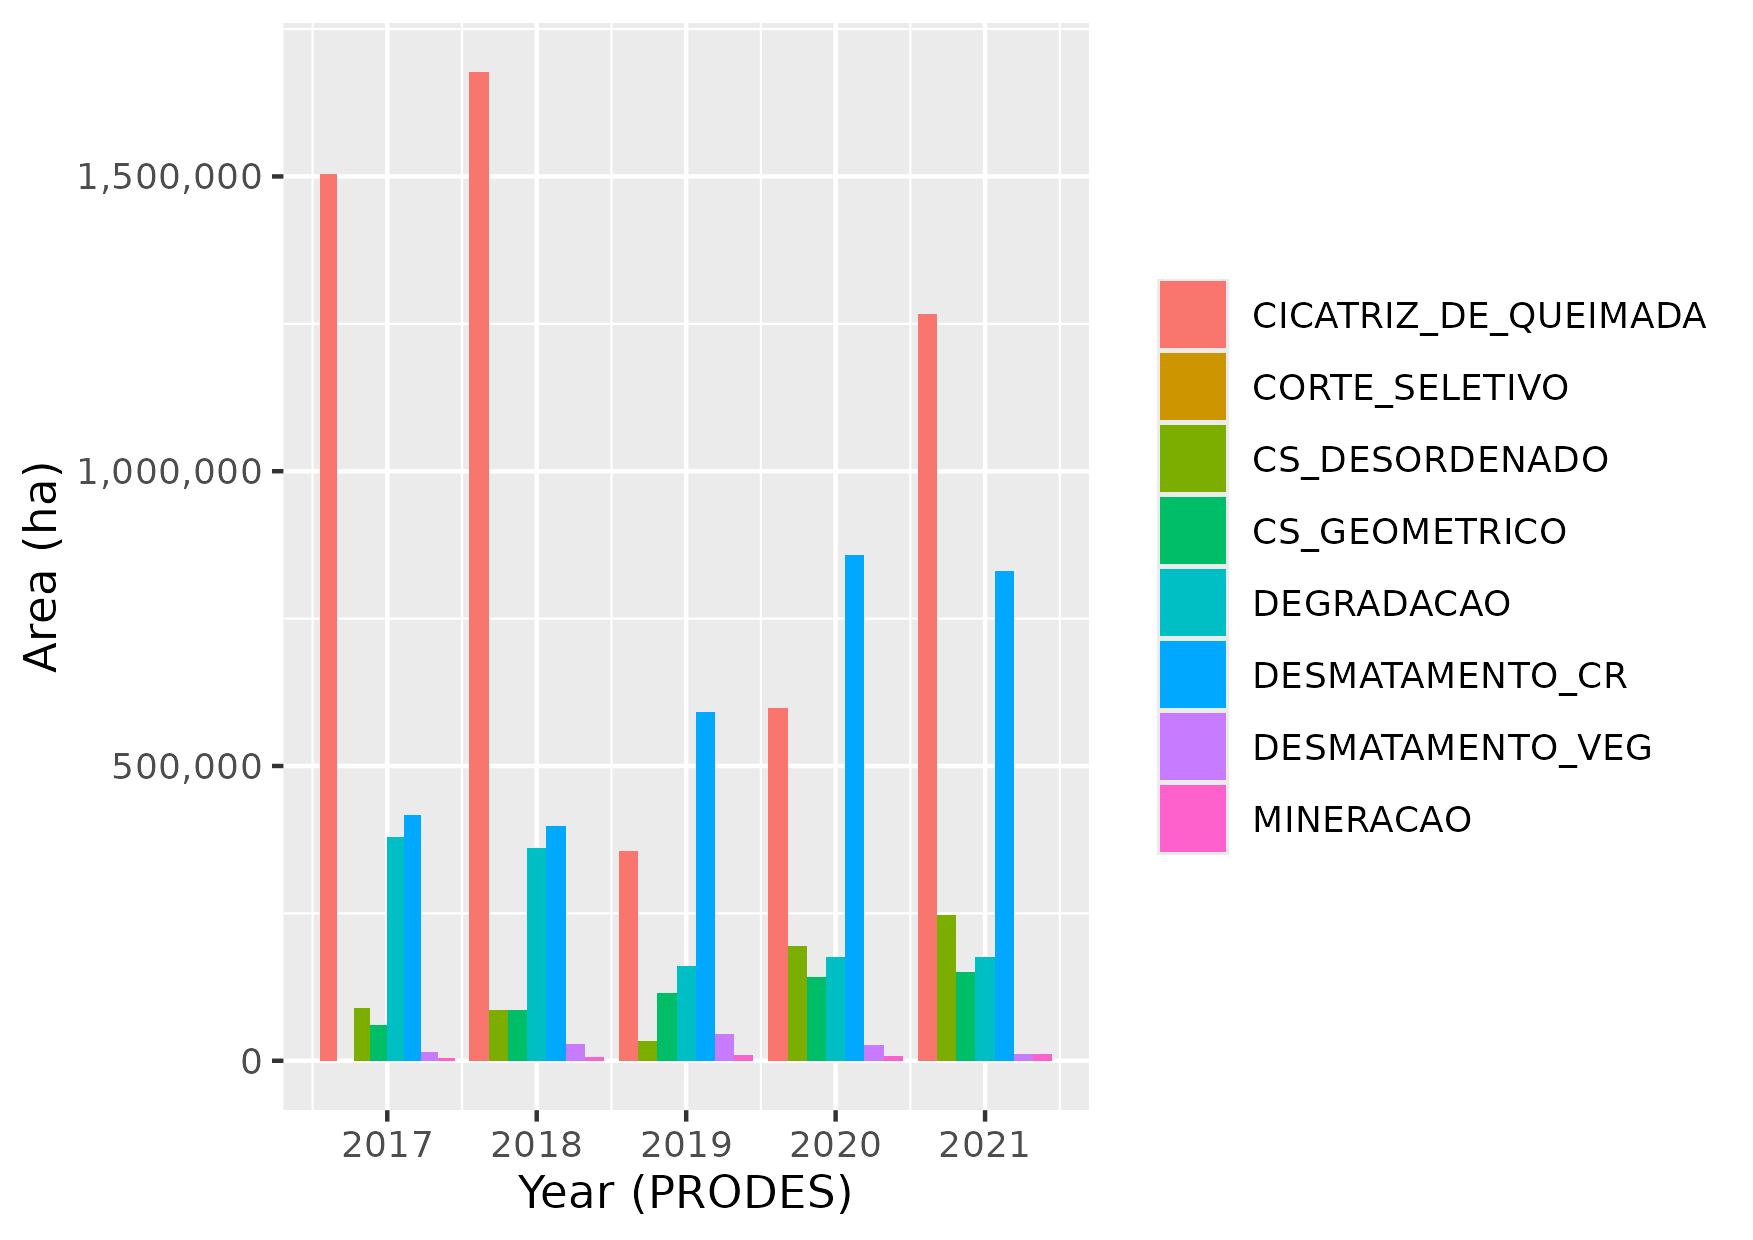
\includegraphics[width=0.75\linewidth]
        {./figures/plot_deter_area_by_class.png}
    \end{figure}
\end{frame}

\begin{frame}
    \frametitle{Area of DETER warnings}
    \begin{figure}[h] 
        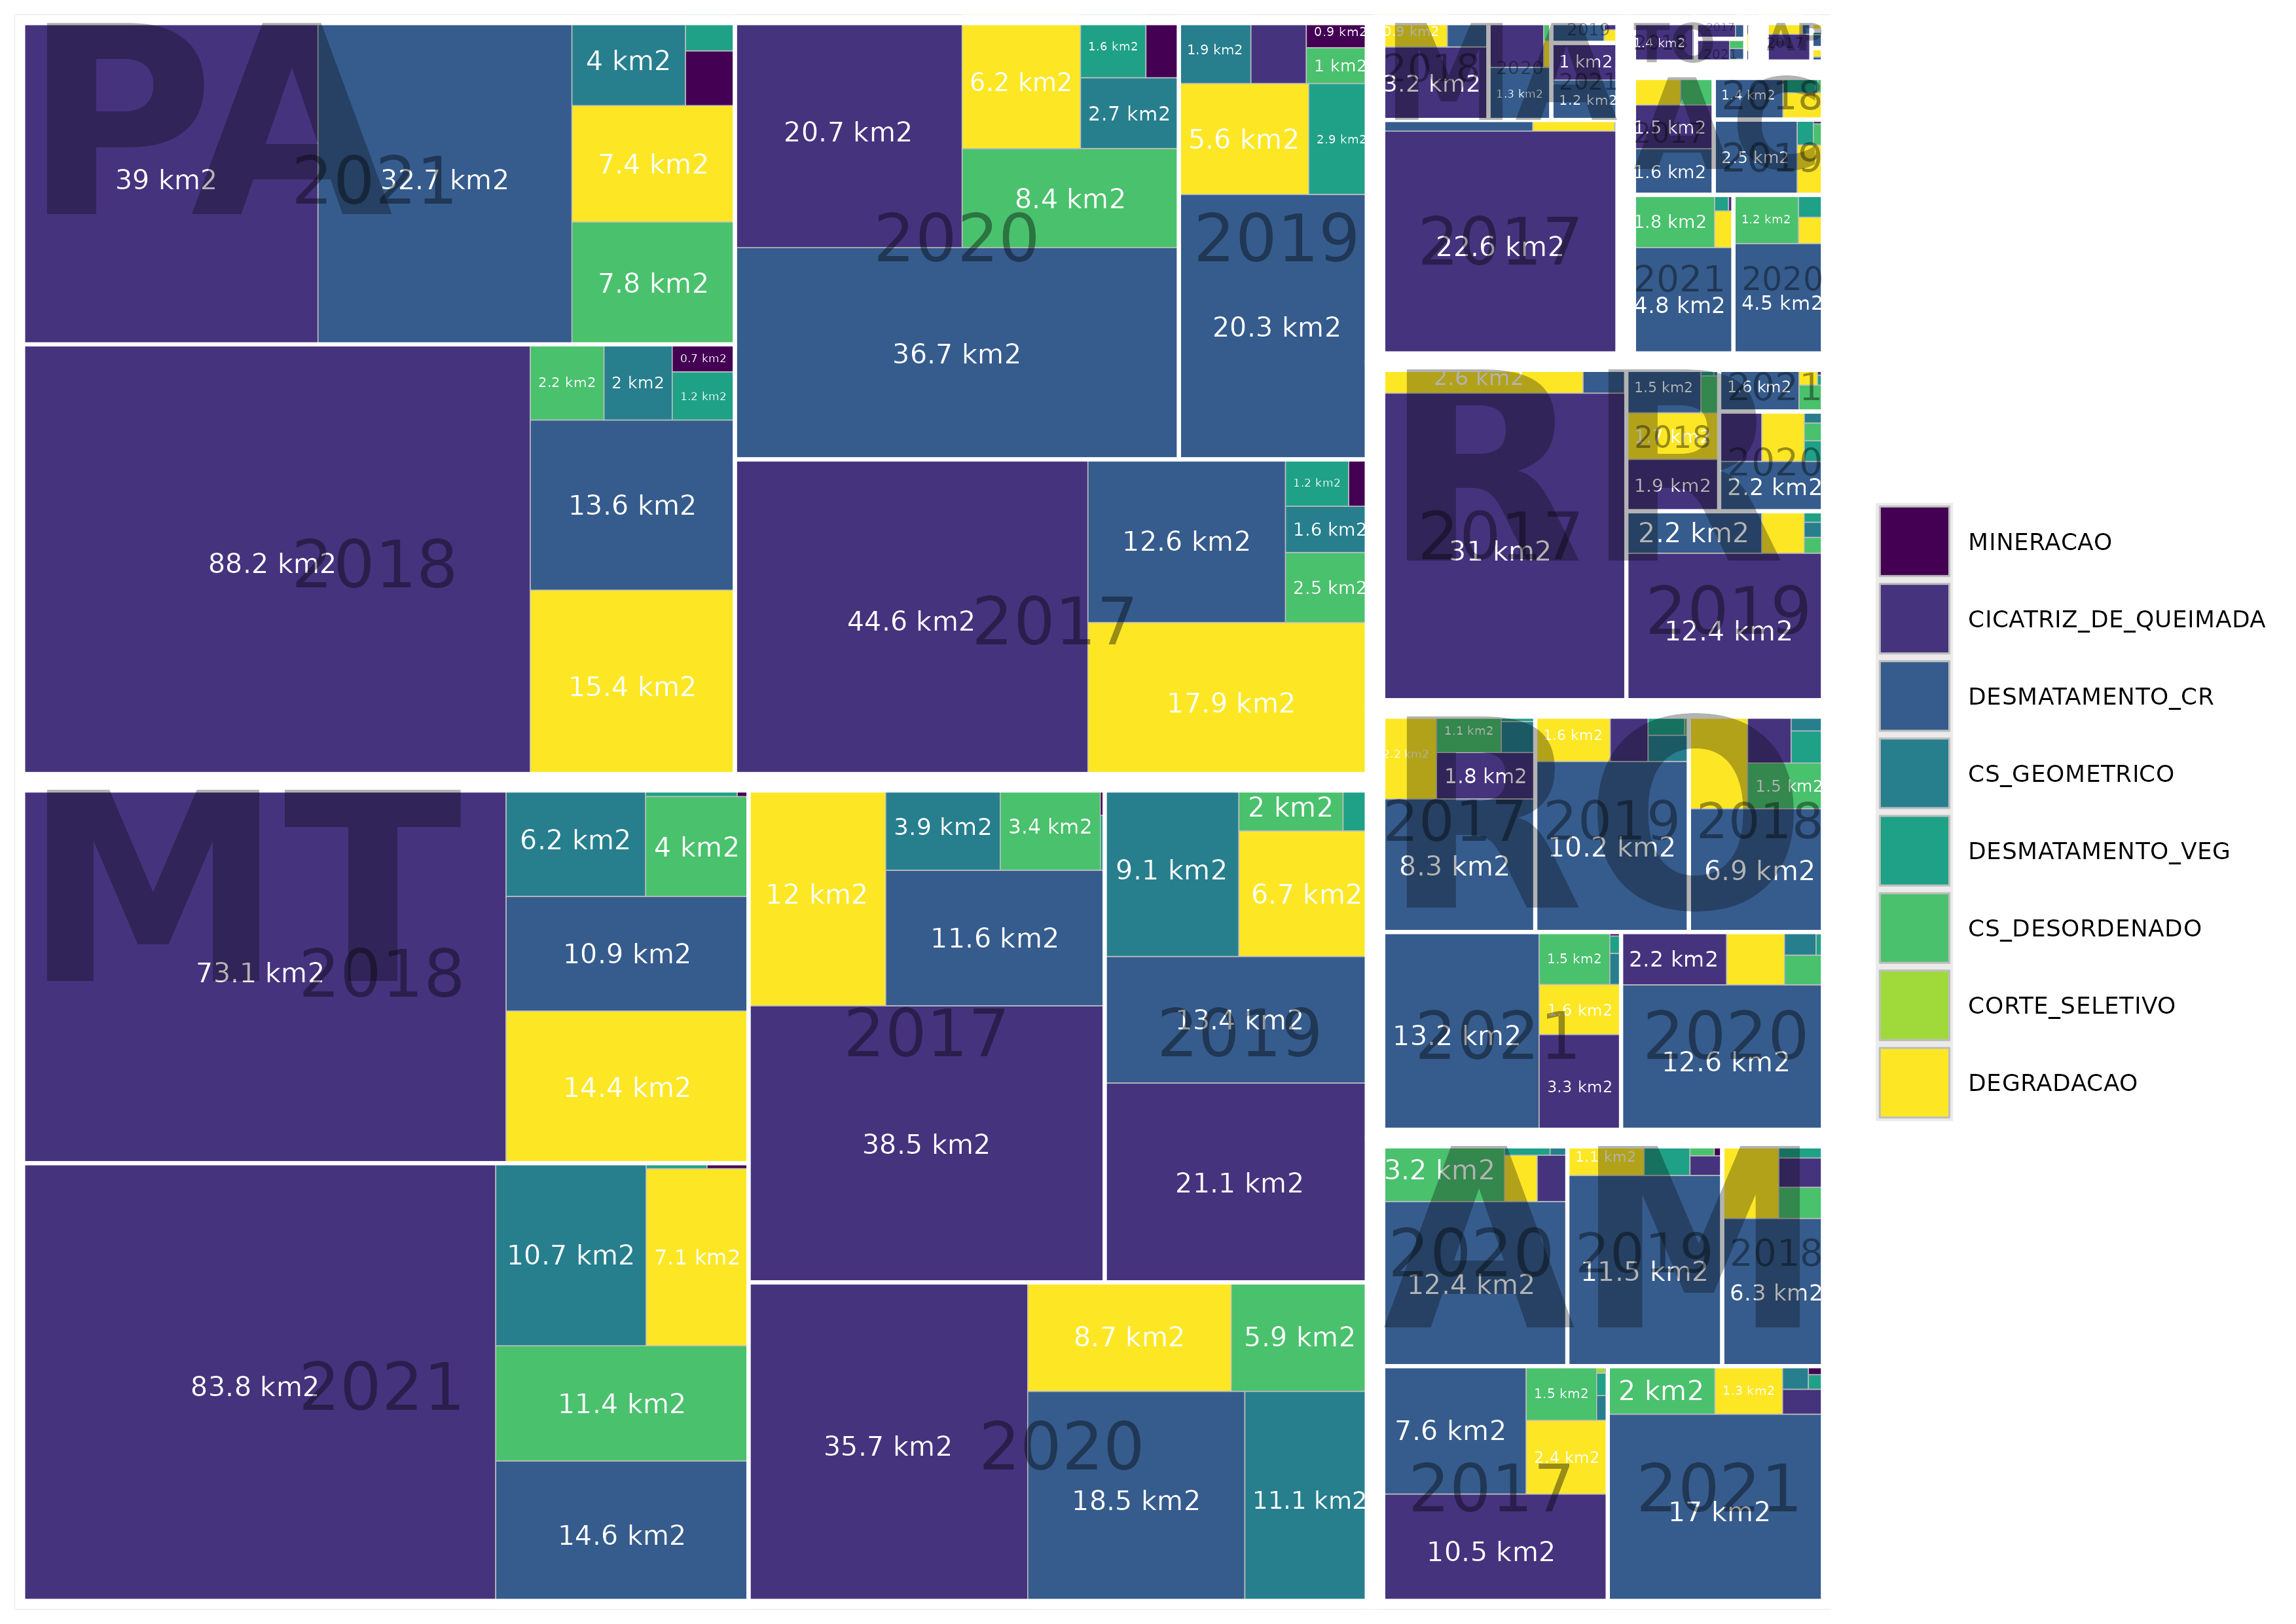
\includegraphics[width=0.75\linewidth]
        {./figures/plot_deter_area_by_state_pyear_type.png}
    \end{figure}
\end{frame}

\begin{frame}
    \frametitle{Area of DETER warnings}
    \begin{figure}[h]
        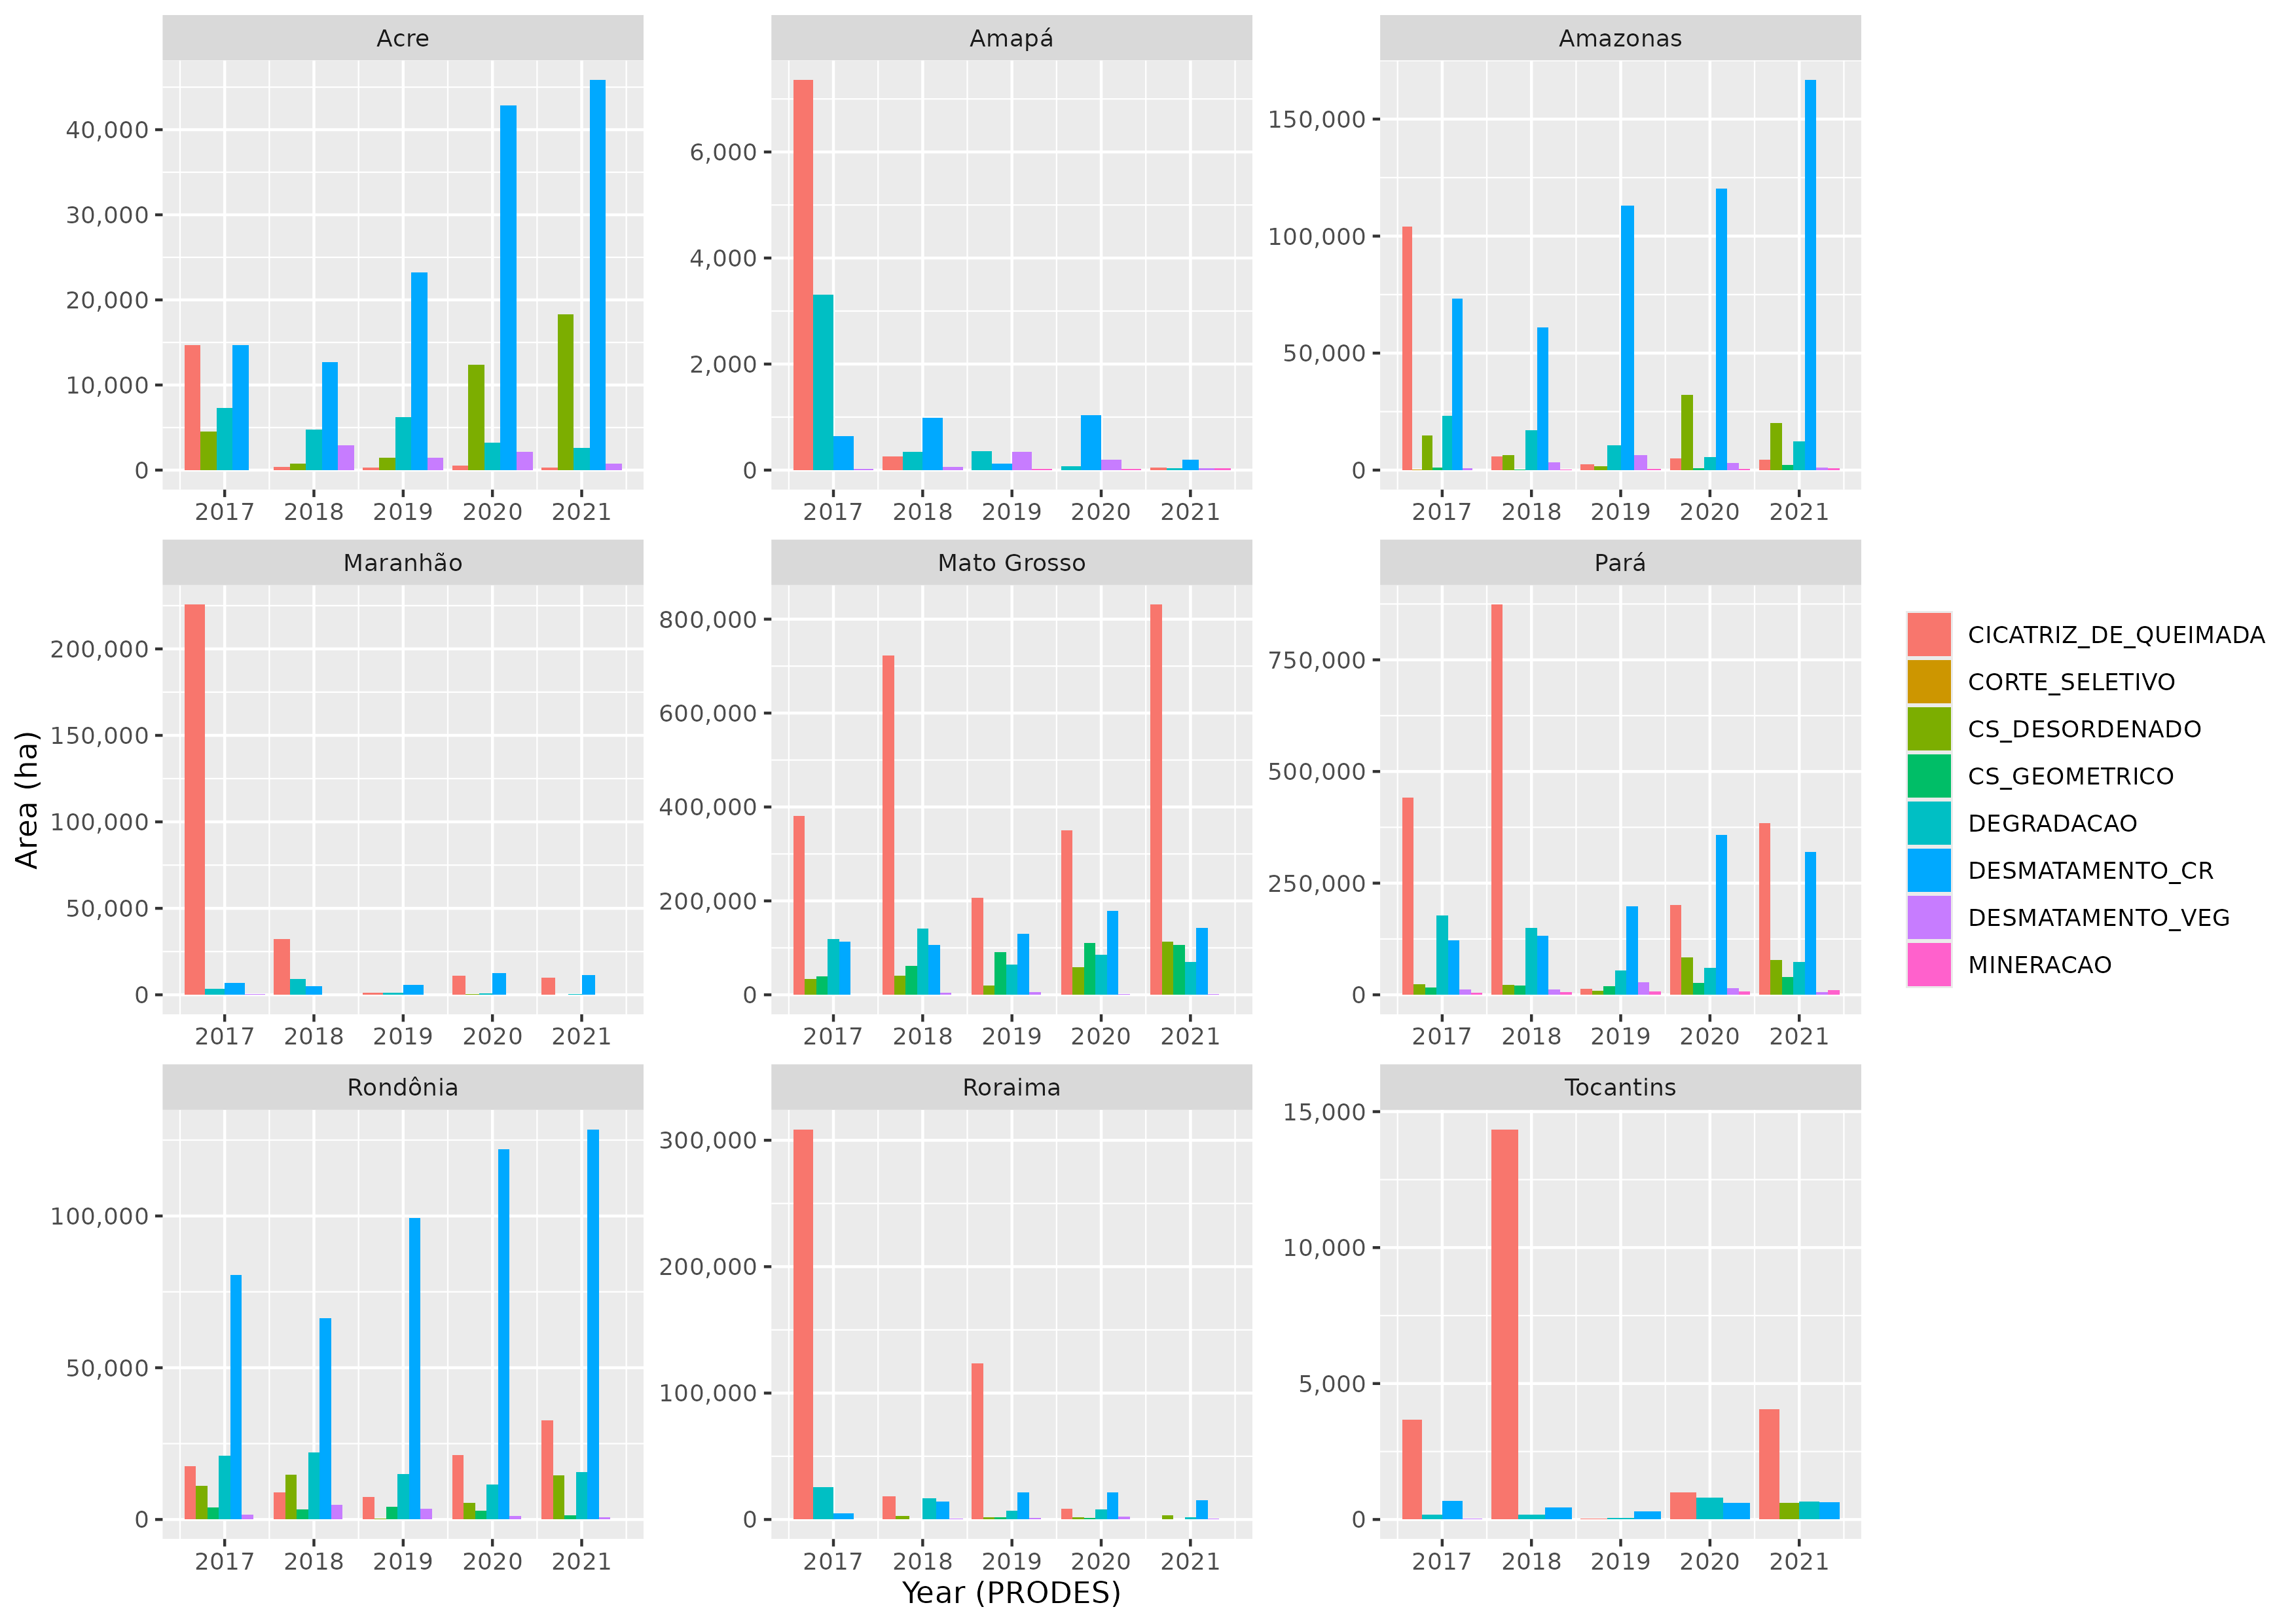
\includegraphics[width=0.75\linewidth]
        {./figures/plot_deter_area_by_class_state.png}
    \end{figure}
\end{frame}

\begin{frame}
    \frametitle{DETER subareas}
    \begin{columns}
        \begin{column}{0.5\textwidth}
            \begin{itemize}
                \item The spatial properties of DETER warnings are inconsistent
                    along time (shape, size, area, position).
                \item On the other hand, DETER subareas maintain keep properties.
                \item Following the example from before, subareas from 3 DETER
                    warnings. we obtained 7 subareas
            \end{itemize}
        \end{column}
        \begin{column}{0.5\textwidth}
            \begin{figure}[h]
                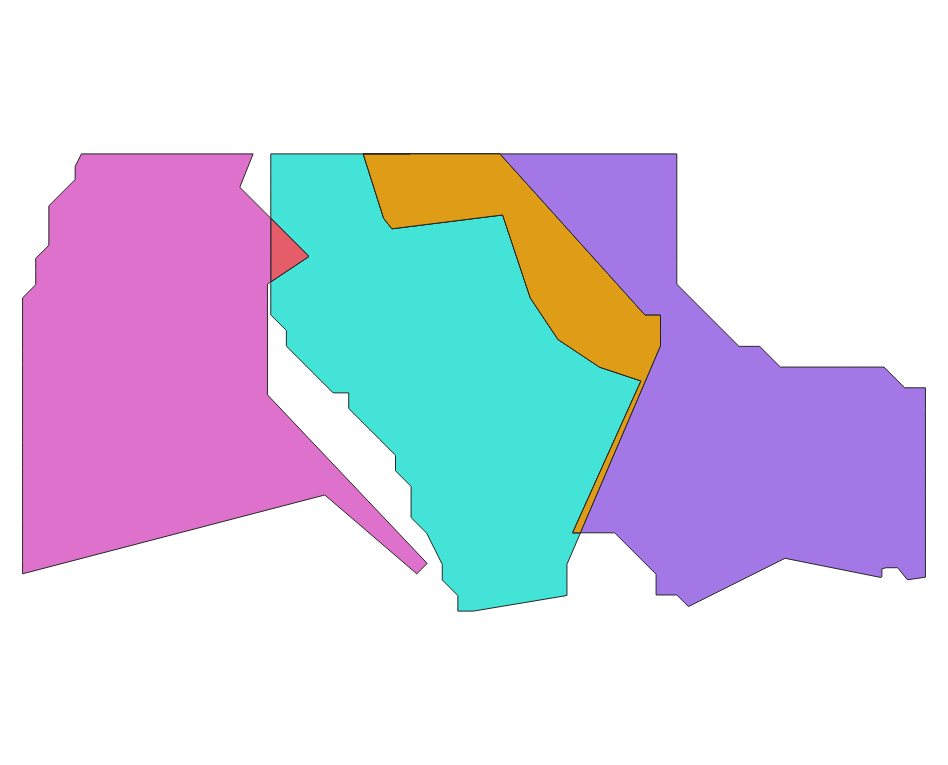
\includegraphics[width=0.99\linewidth]
                {./images/sample_deter_subareas.png}
            \end{figure}
        \end{column}
    \end{columns}
\end{frame}

\section{Results}

\subsection{Exploratory data analysis}

\begin{frame}
    \frametitle{Subareas by number of warnings}
    \begin{figure}[h]
        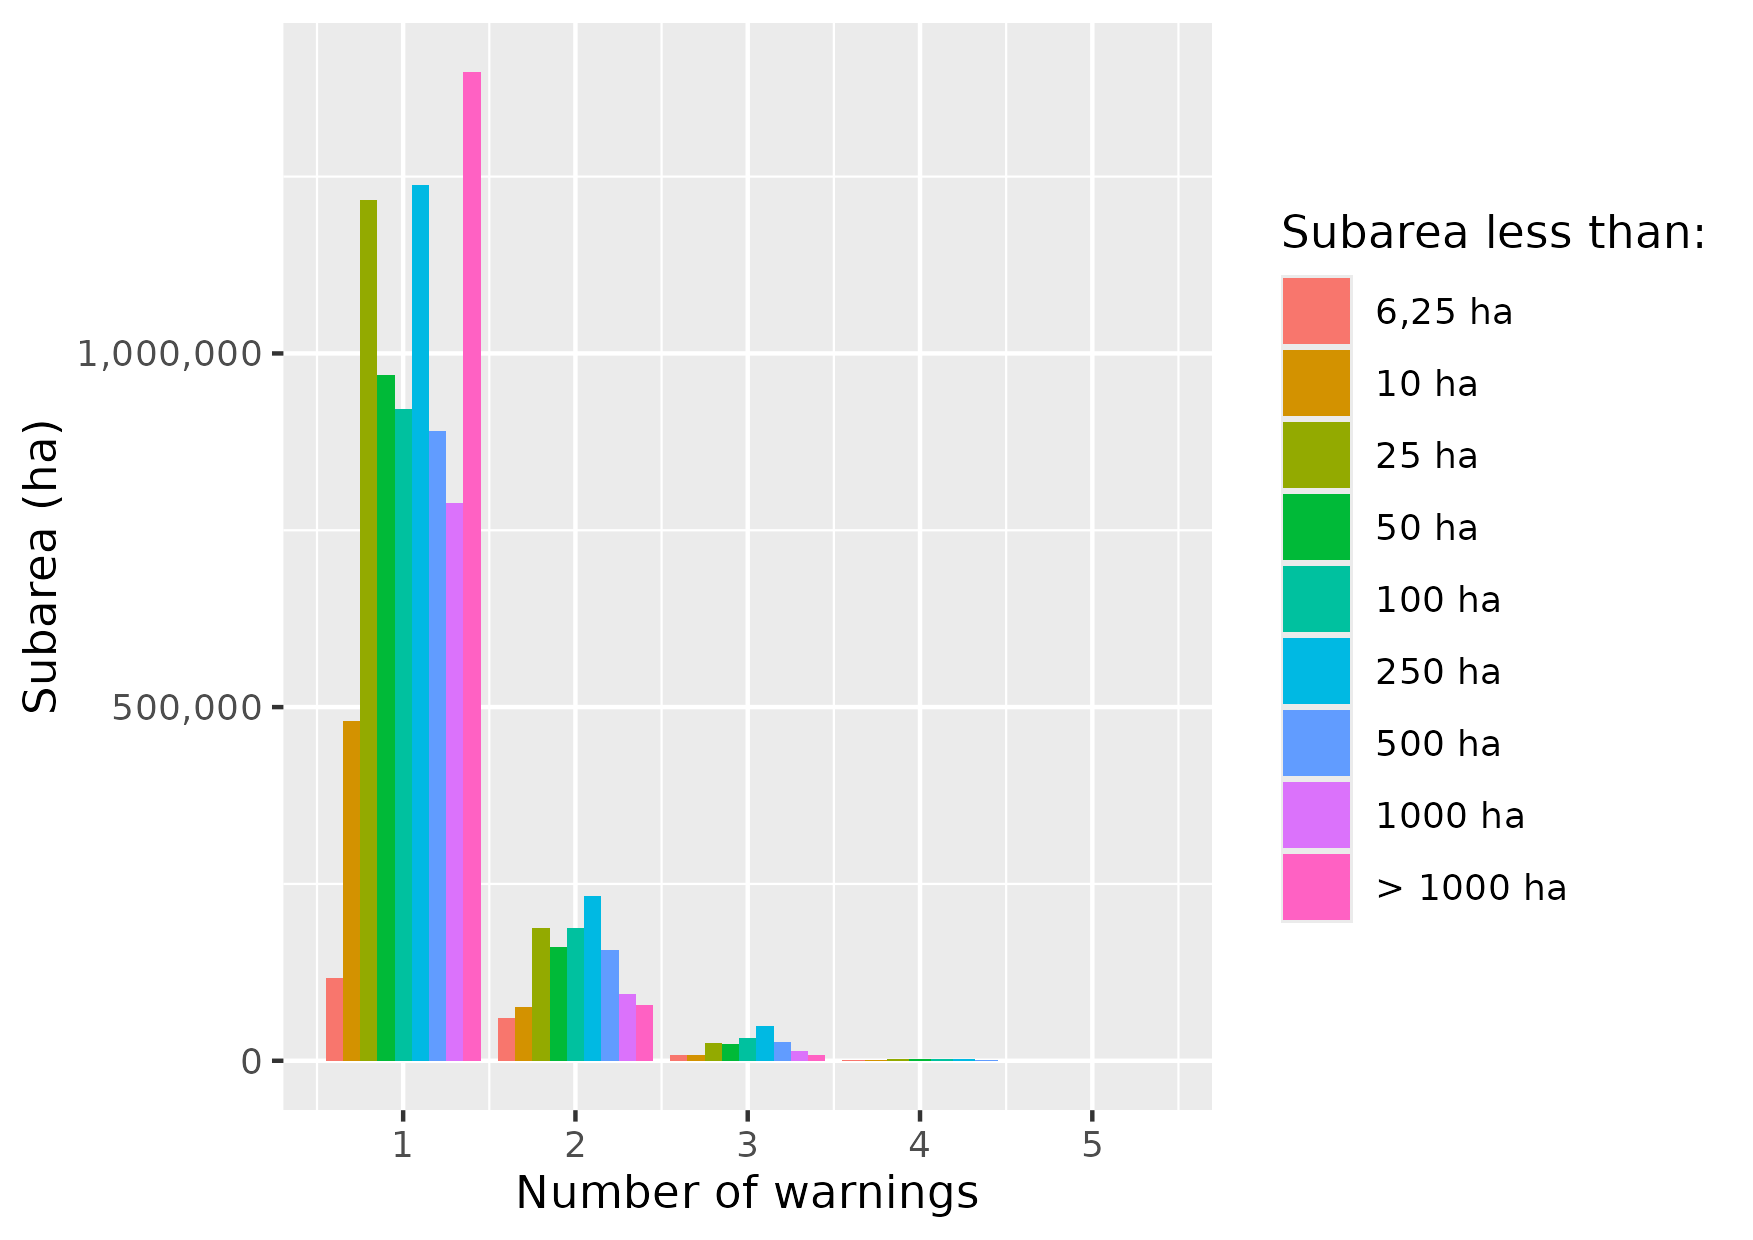
\includegraphics[width=0.70\linewidth]
        {./figures/plot_deter_subarea_by_nwarnings.png}
    \end{figure}
\end{frame}

\begin{frame}
    \frametitle{Subareas by number of warnings}
    \begin{figure}[h]
        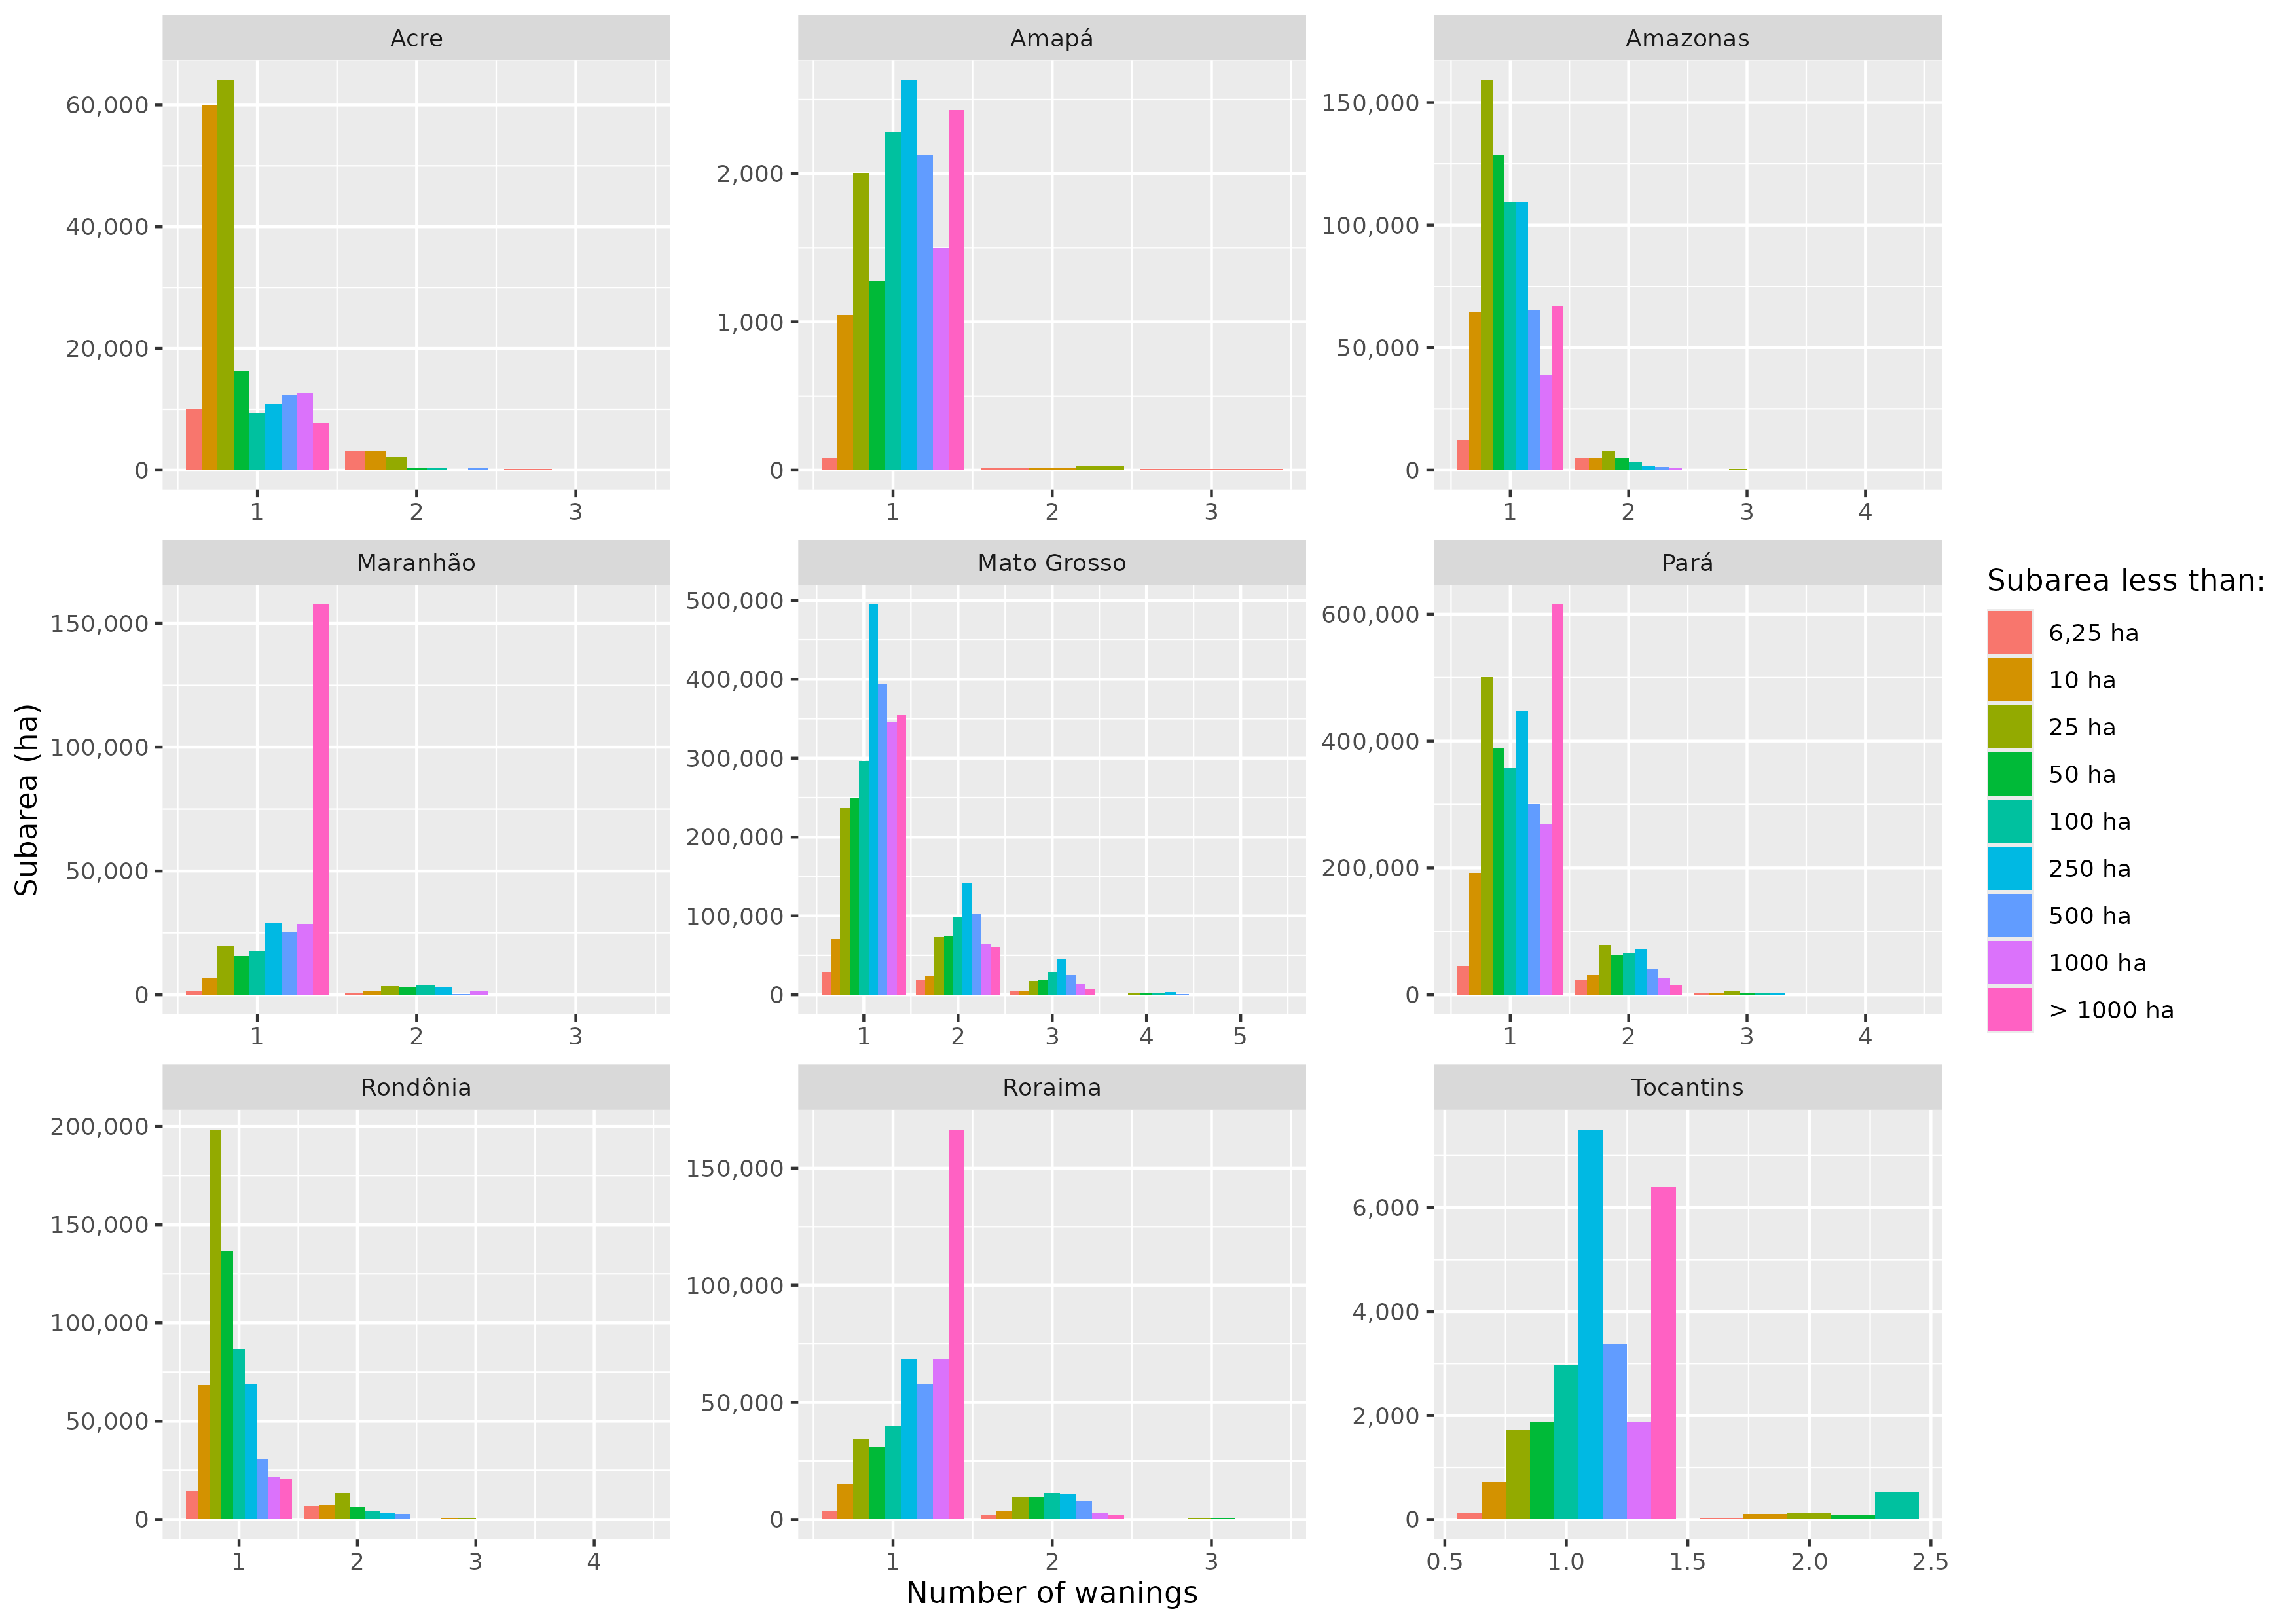
\includegraphics[width=0.70\linewidth]
        {./figures/plot_deter_subarea_by_warnings_state.png}
    \end{figure}
\end{frame}

\begin{frame}
    \frametitle{Subareas by number of warnings}
    \begin{figure}[h]
        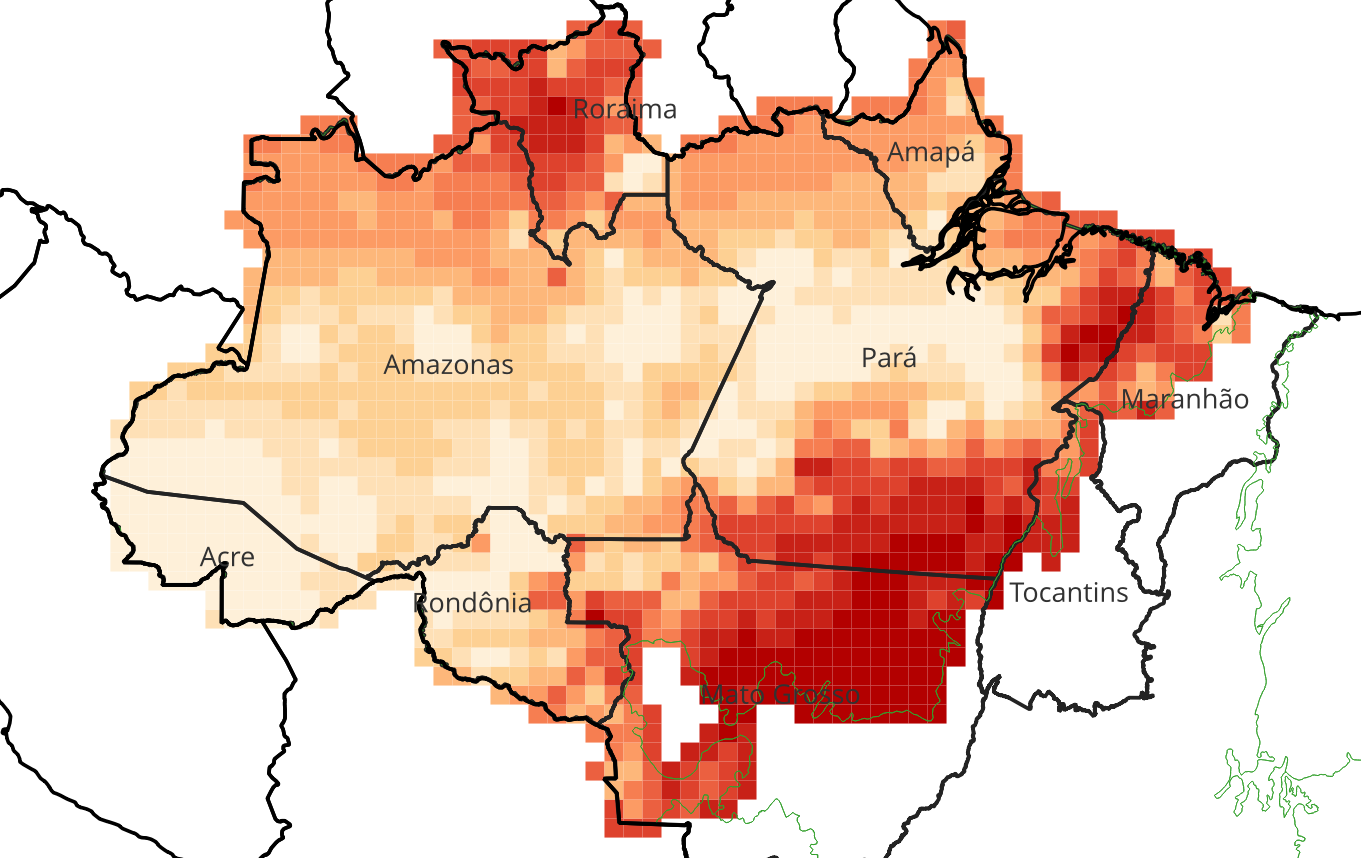
\includegraphics[width=0.70\linewidth]
        {./images/nwarnings_idw_map.png}
    \end{figure}
\end{frame}

\begin{frame}
    \frametitle{Days from first to last warning}
    \begin{figure}[h]
        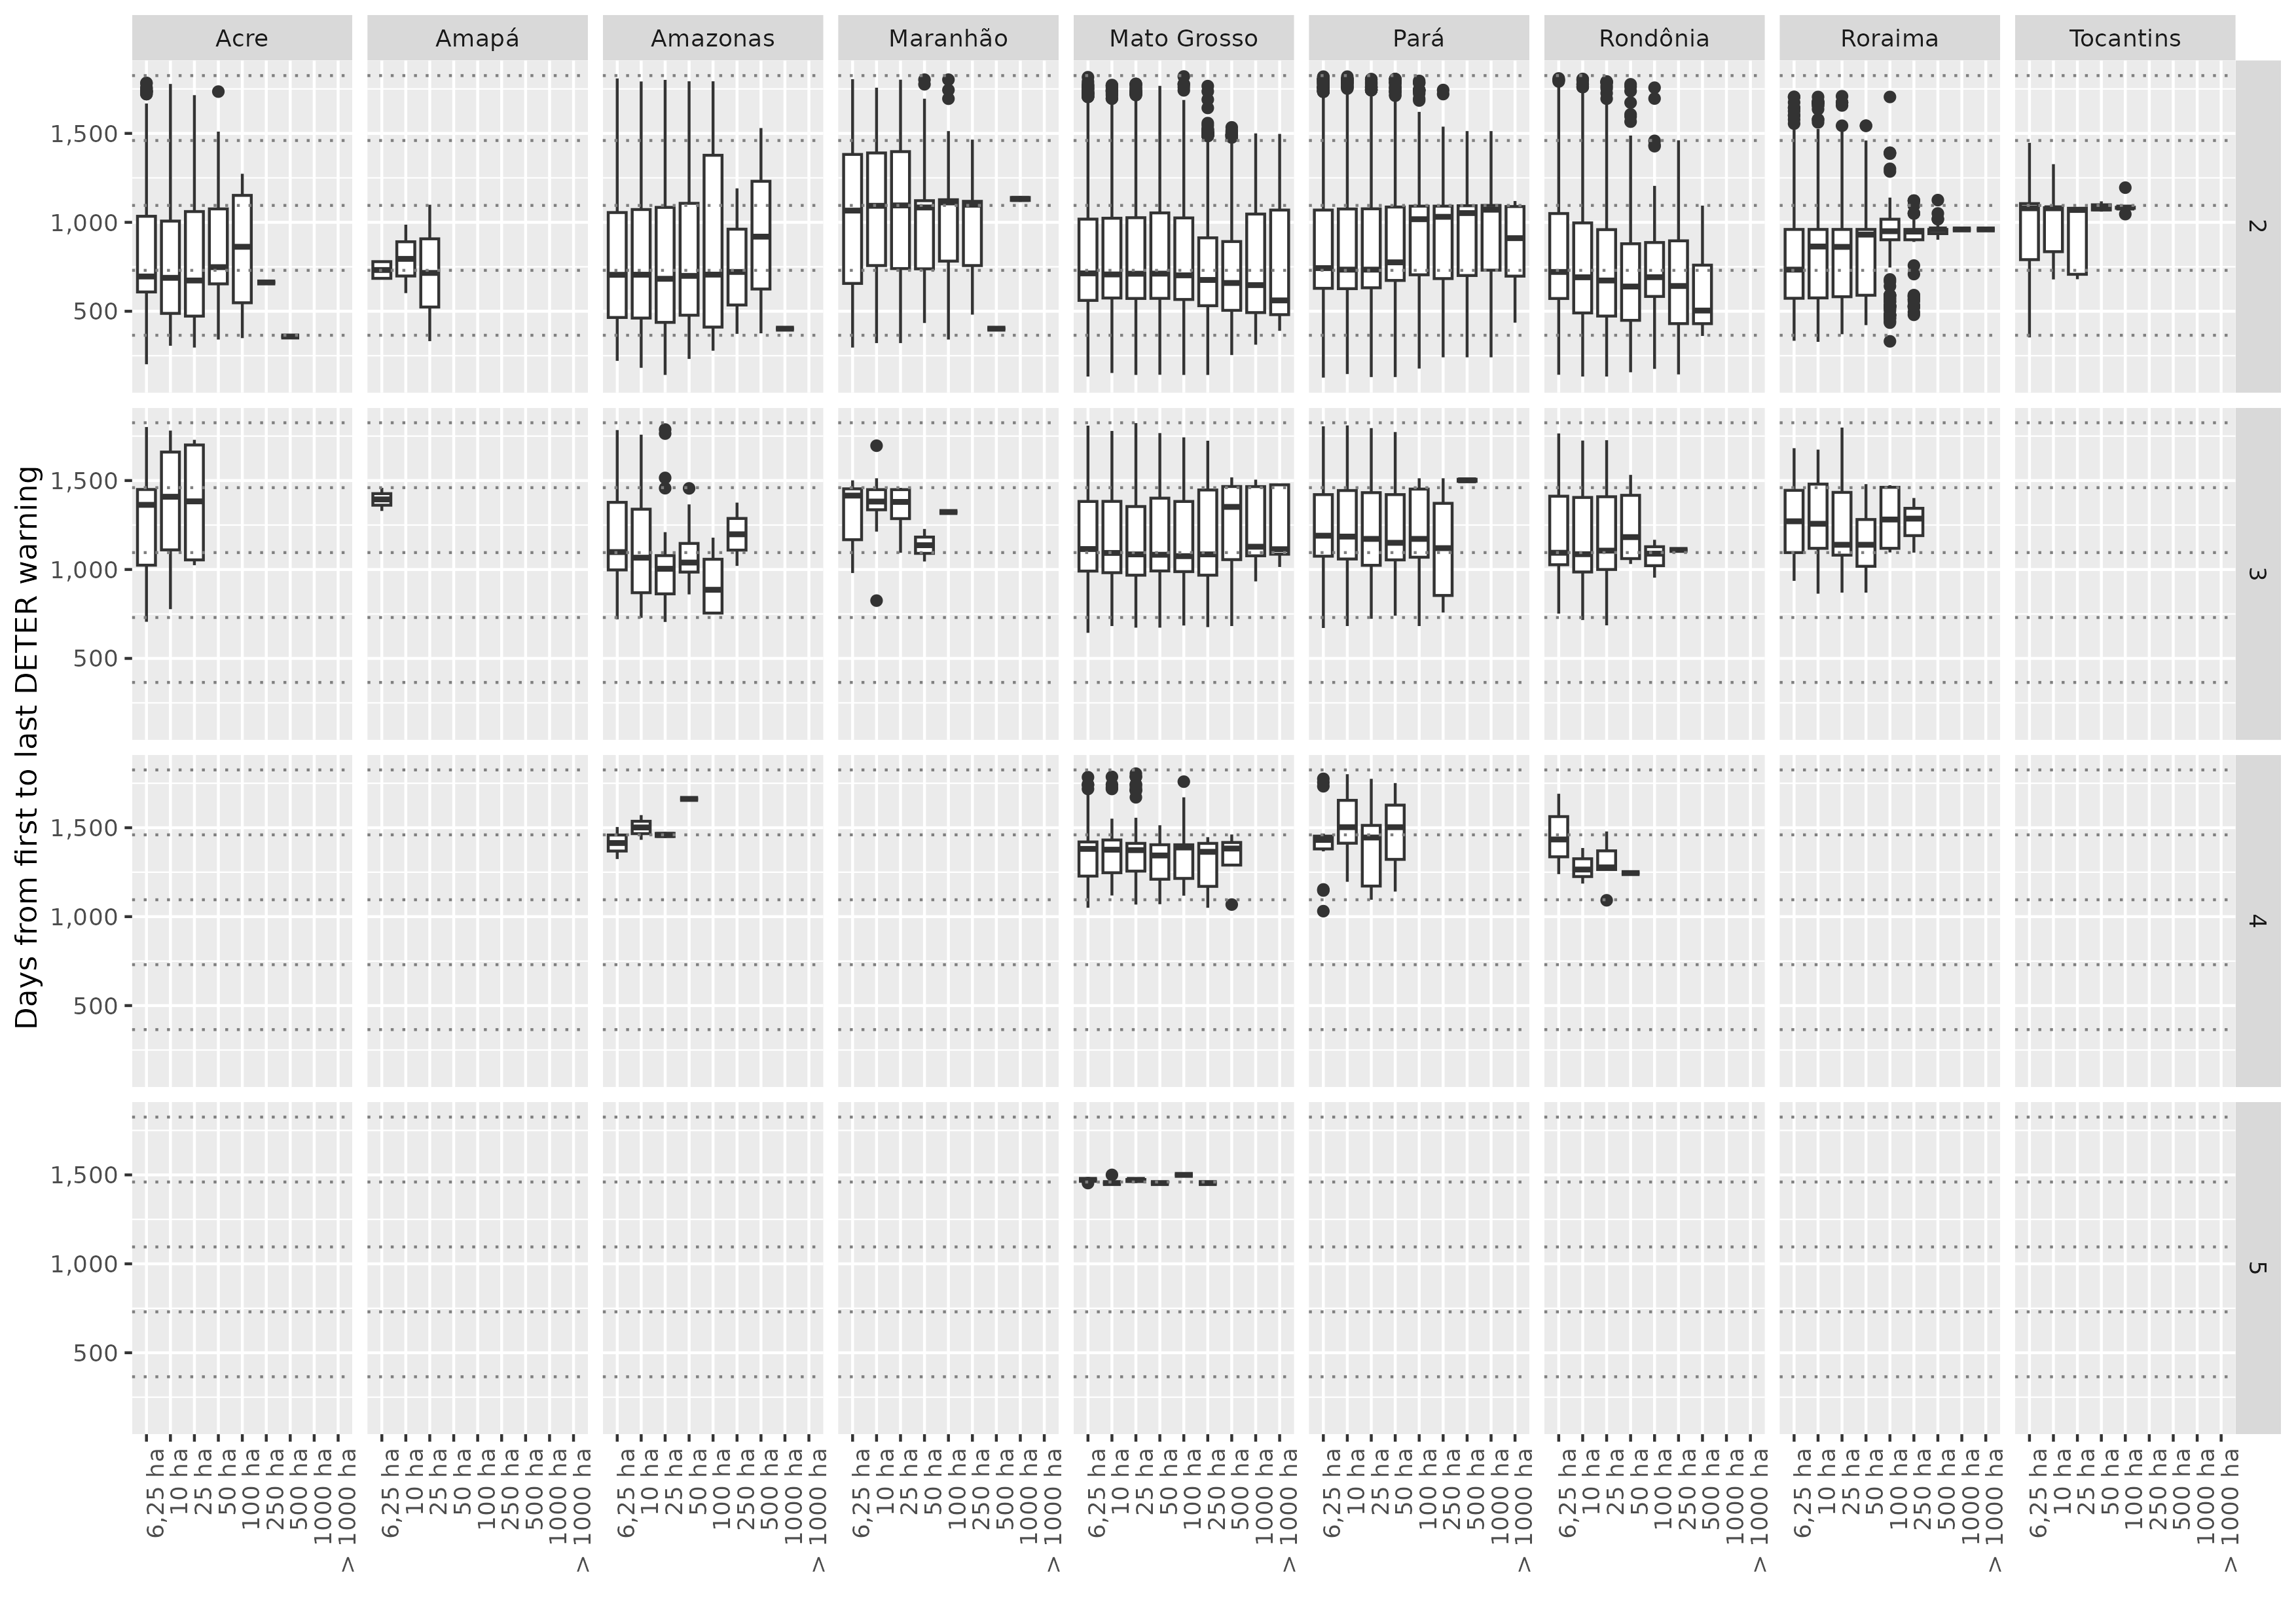
\includegraphics[width=0.75\linewidth]
        {./figures/plot_deter_days_first_to_last.png}
    \end{figure}
\end{frame}

\begin{frame}
    \frametitle{Days from first to last warning (zoom)}
    \begin{figure}[h]
        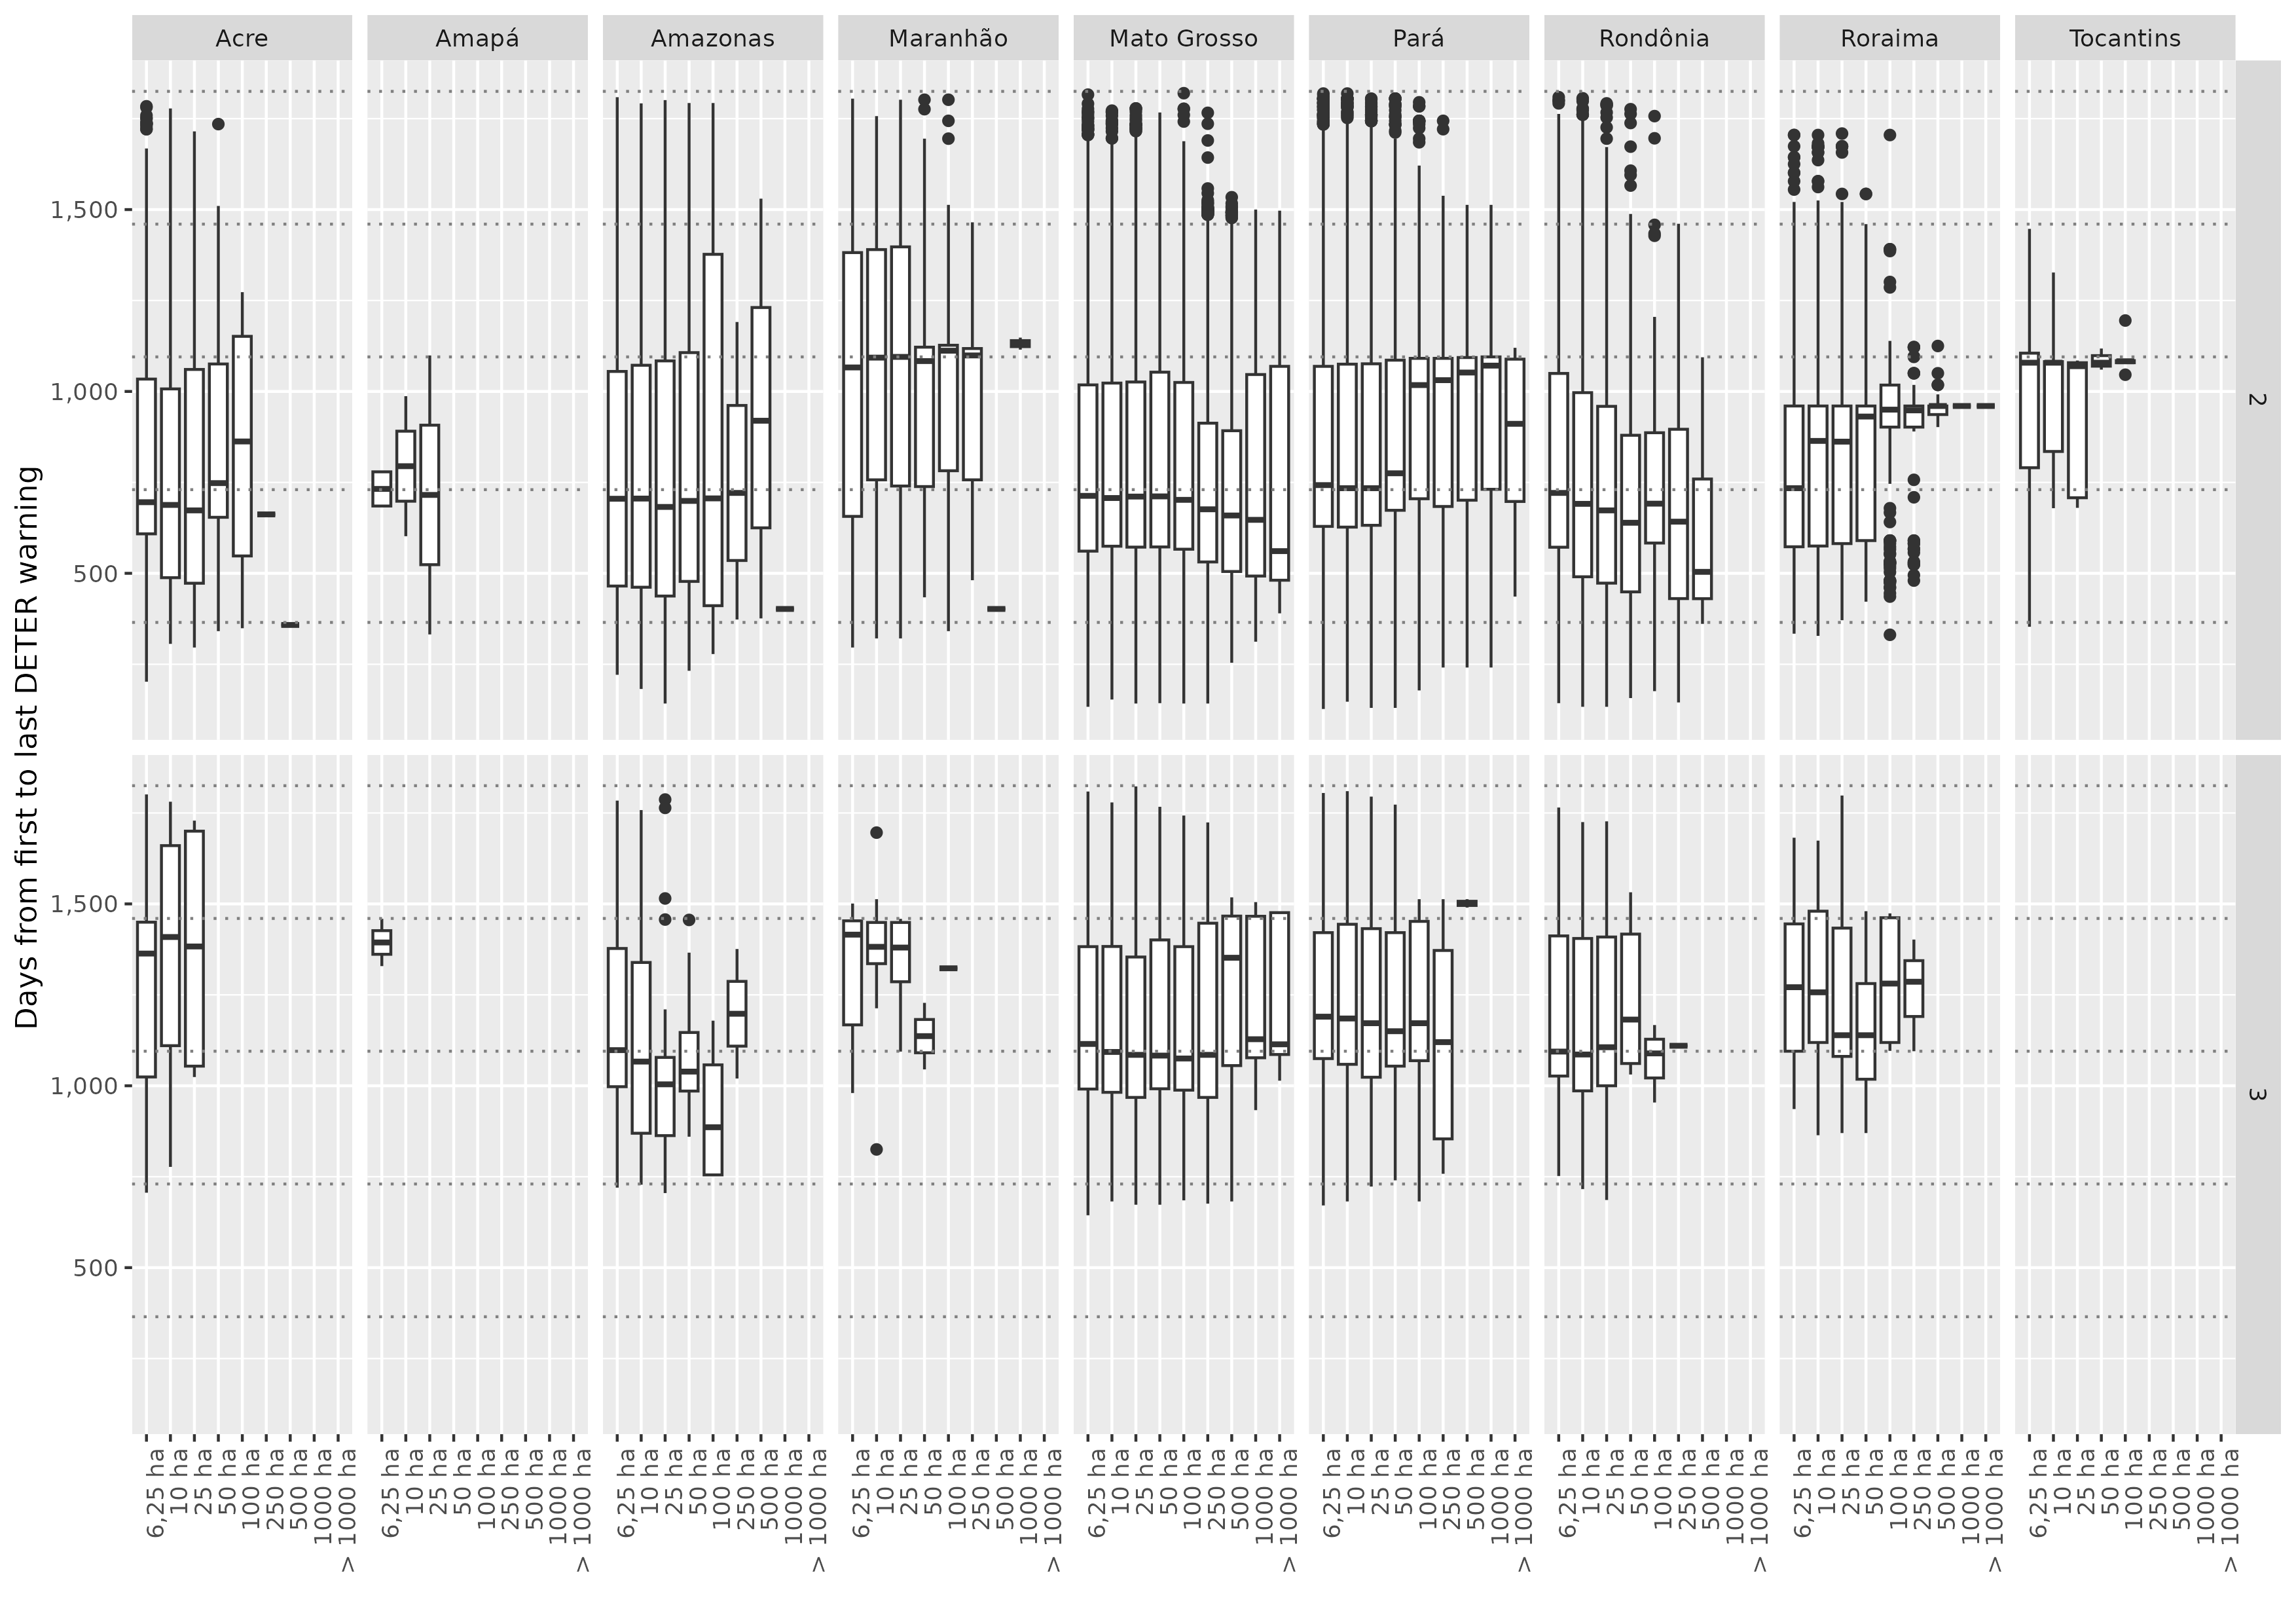
\includegraphics[width=0.75\linewidth]
        {./figures/plot_deter_days_first_to_last_zoom.png}
    \end{figure}
\end{frame}

\begin{frame}
    \frametitle{Days between warnings}
    \begin{figure}[h]
        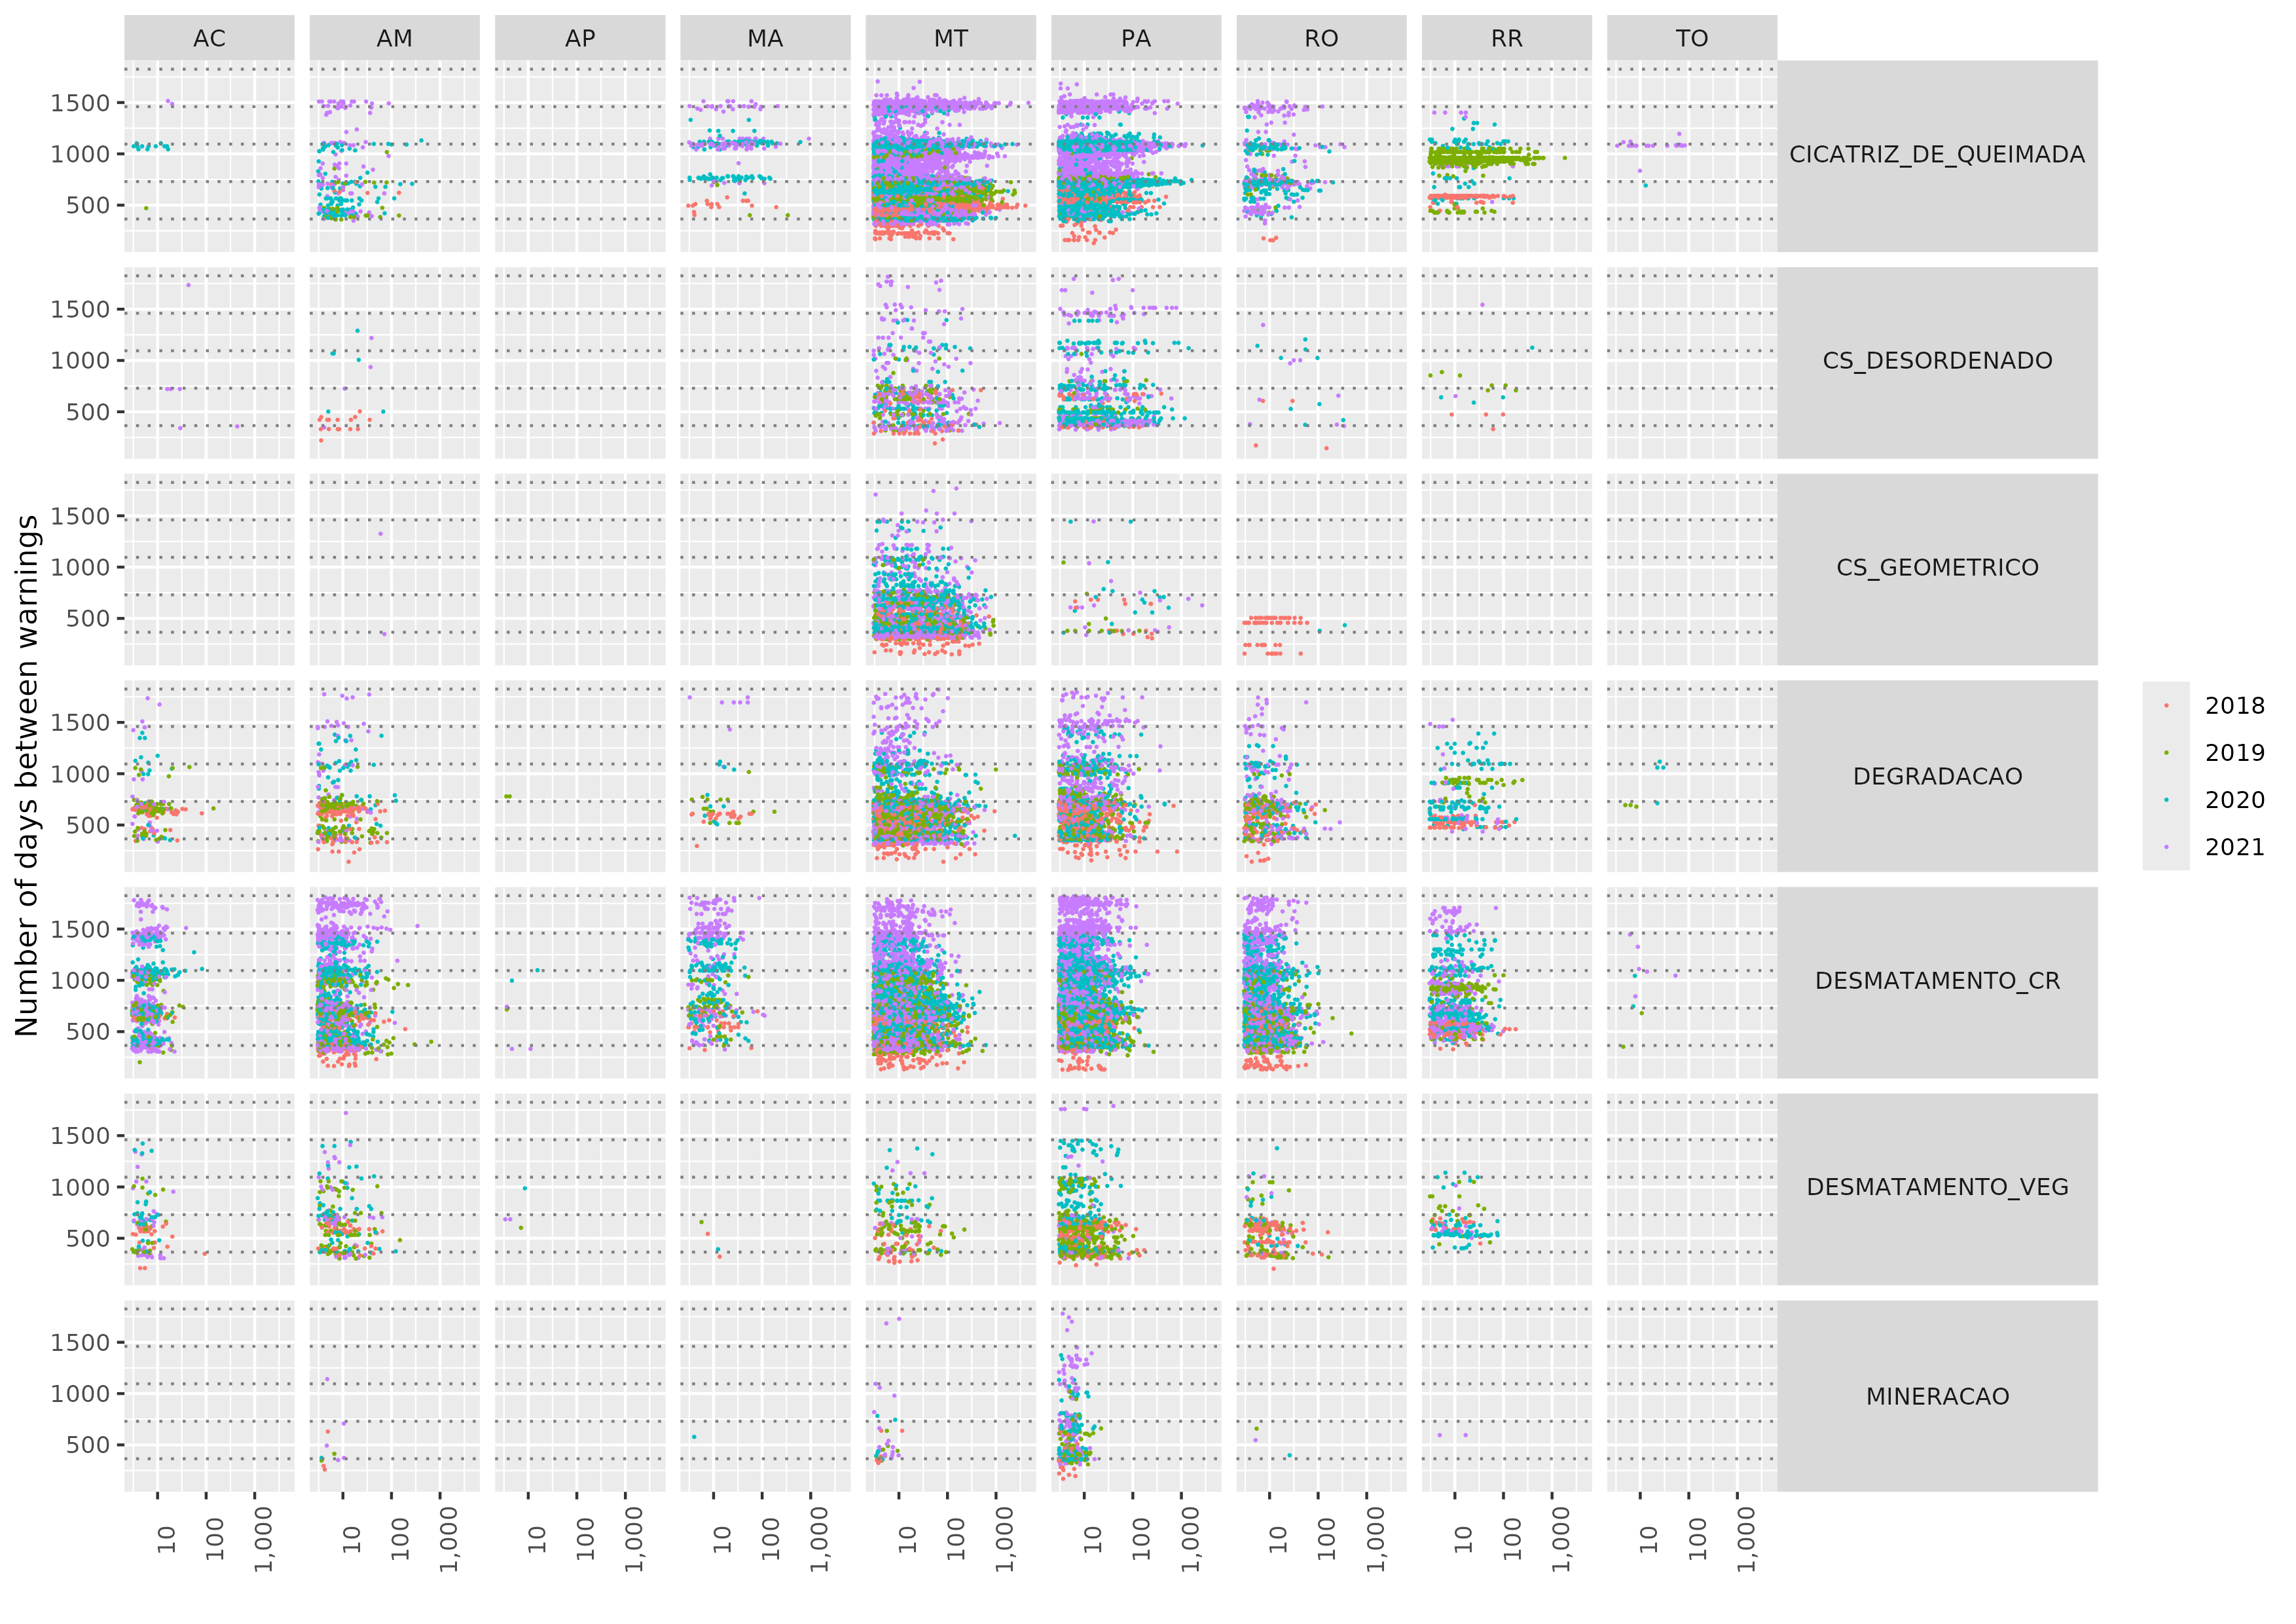
\includegraphics[width=0.75\linewidth]
        {./figures/plot_deter_subarea_density_by_state_first-type_nwarnings.png}
    \end{figure}
\end{frame}

\begin{frame}
    \frametitle{Days between warnings (zoom)}
    \begin{figure}[h]
        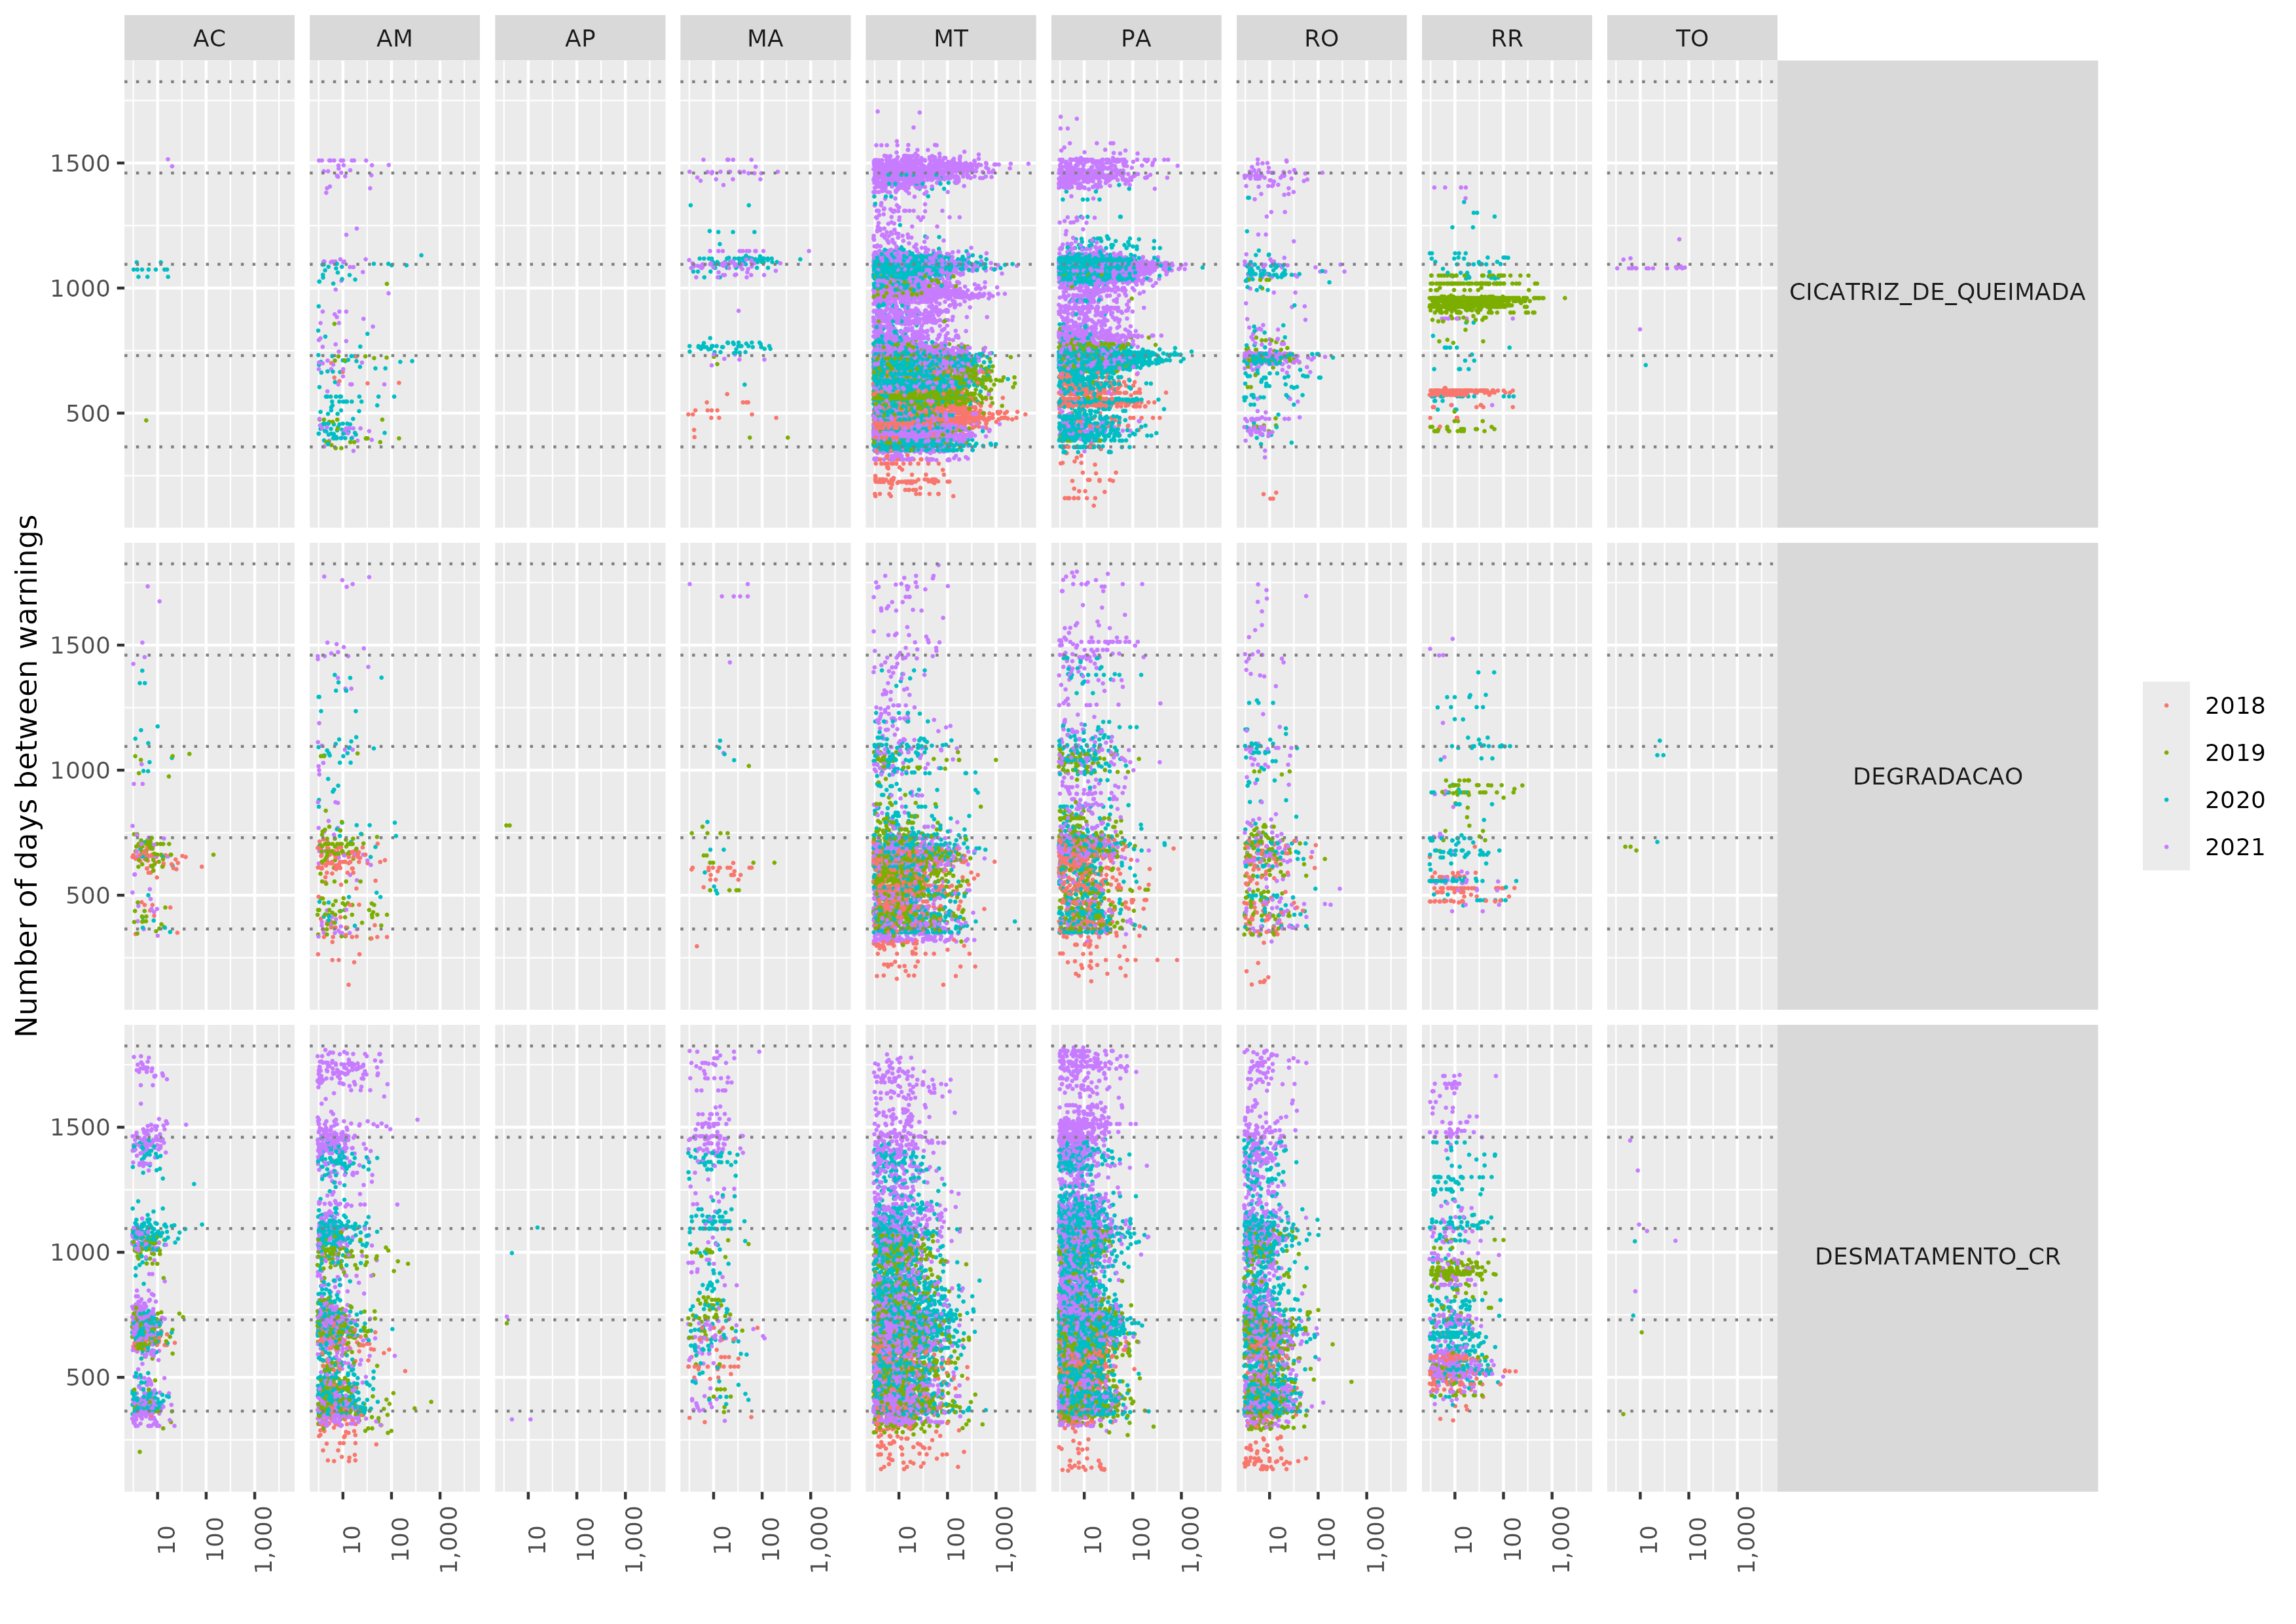
\includegraphics[width=0.75\linewidth]
        {./figures/plot_deter_subarea_density_by_state_first-type_nwarnings_zoom.png}
    \end{figure}
\end{frame}

\subsection{Trajectories}

\begin{frame}
    \frametitle{Subarea trajectories (2 warnings)}
    \begin{figure}[h]
        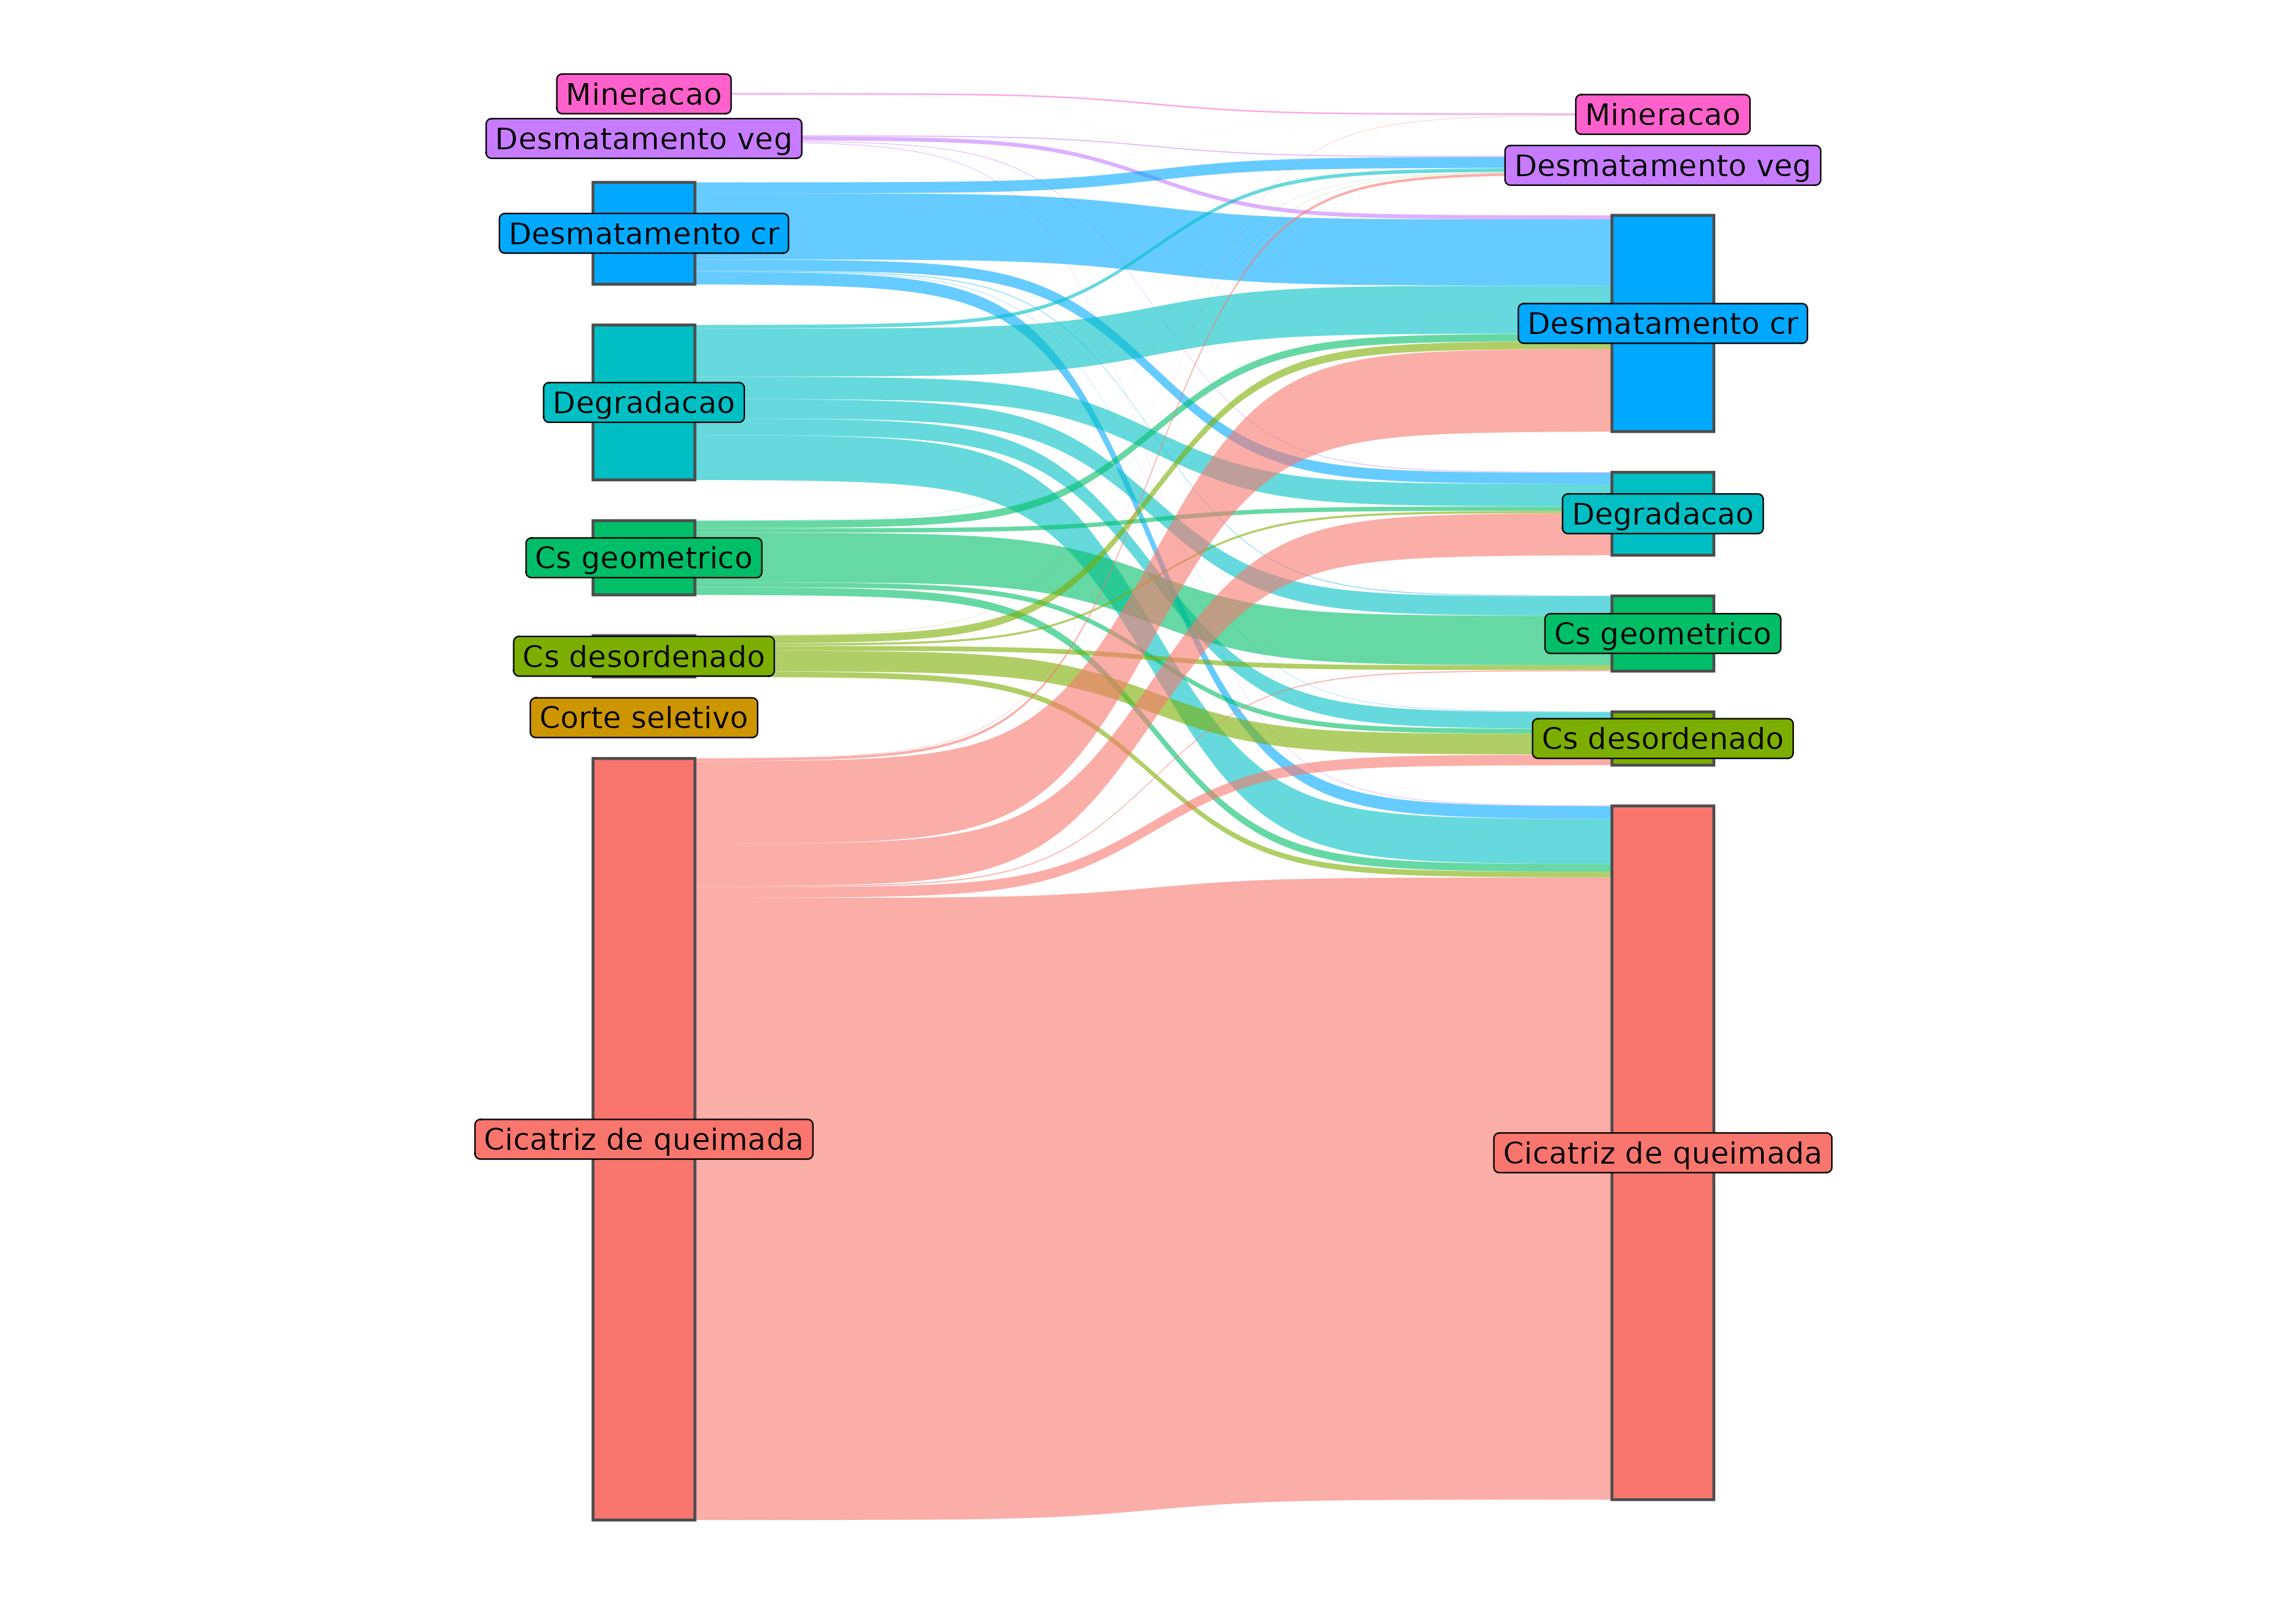
\includegraphics[width=0.75\linewidth]
        {./figures/plot_deter_subarea_trajectory_2.png}
    \end{figure}
\end{frame}

\begin{frame}
    \frametitle{Subarea trajectories (3 warnings)}
    \begin{figure}[h]
        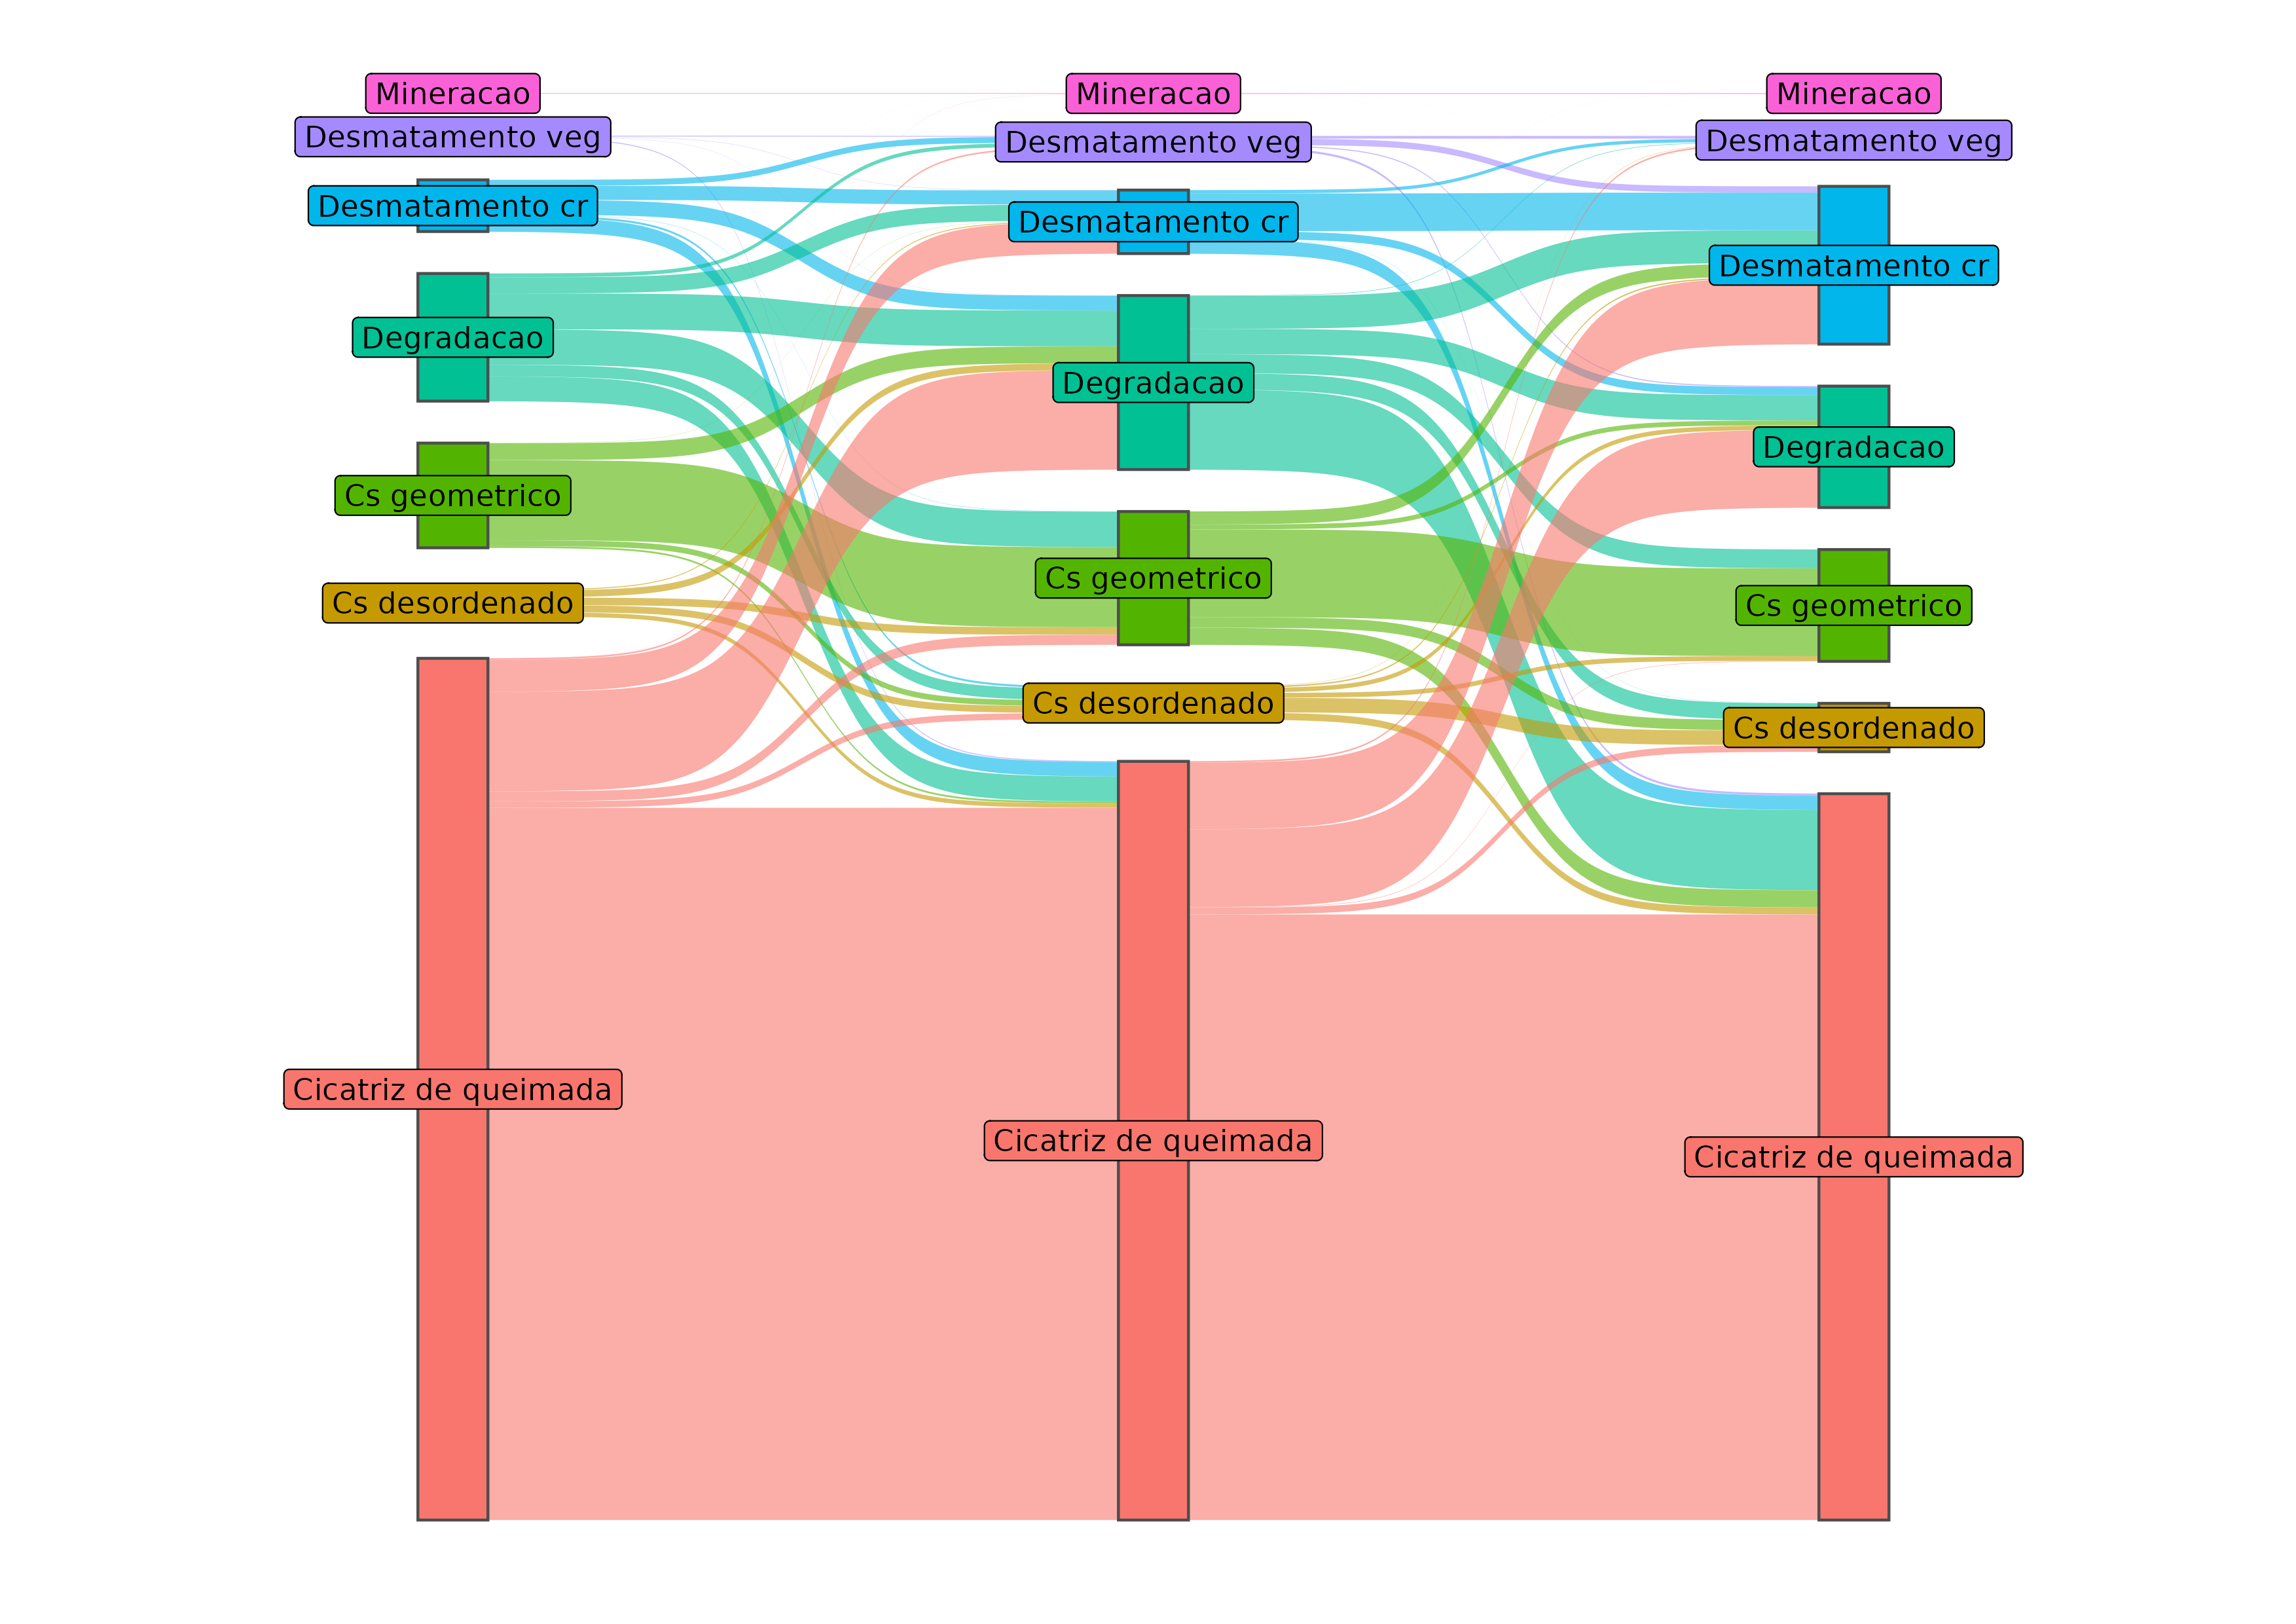
\includegraphics[width=0.75\linewidth]
        {./figures/plot_deter_subarea_trajectory_3.png}
    \end{figure}
\end{frame}

\begin{frame}
    \frametitle{Subarea trajectories (4 warnings)}
    \begin{figure}[h]
        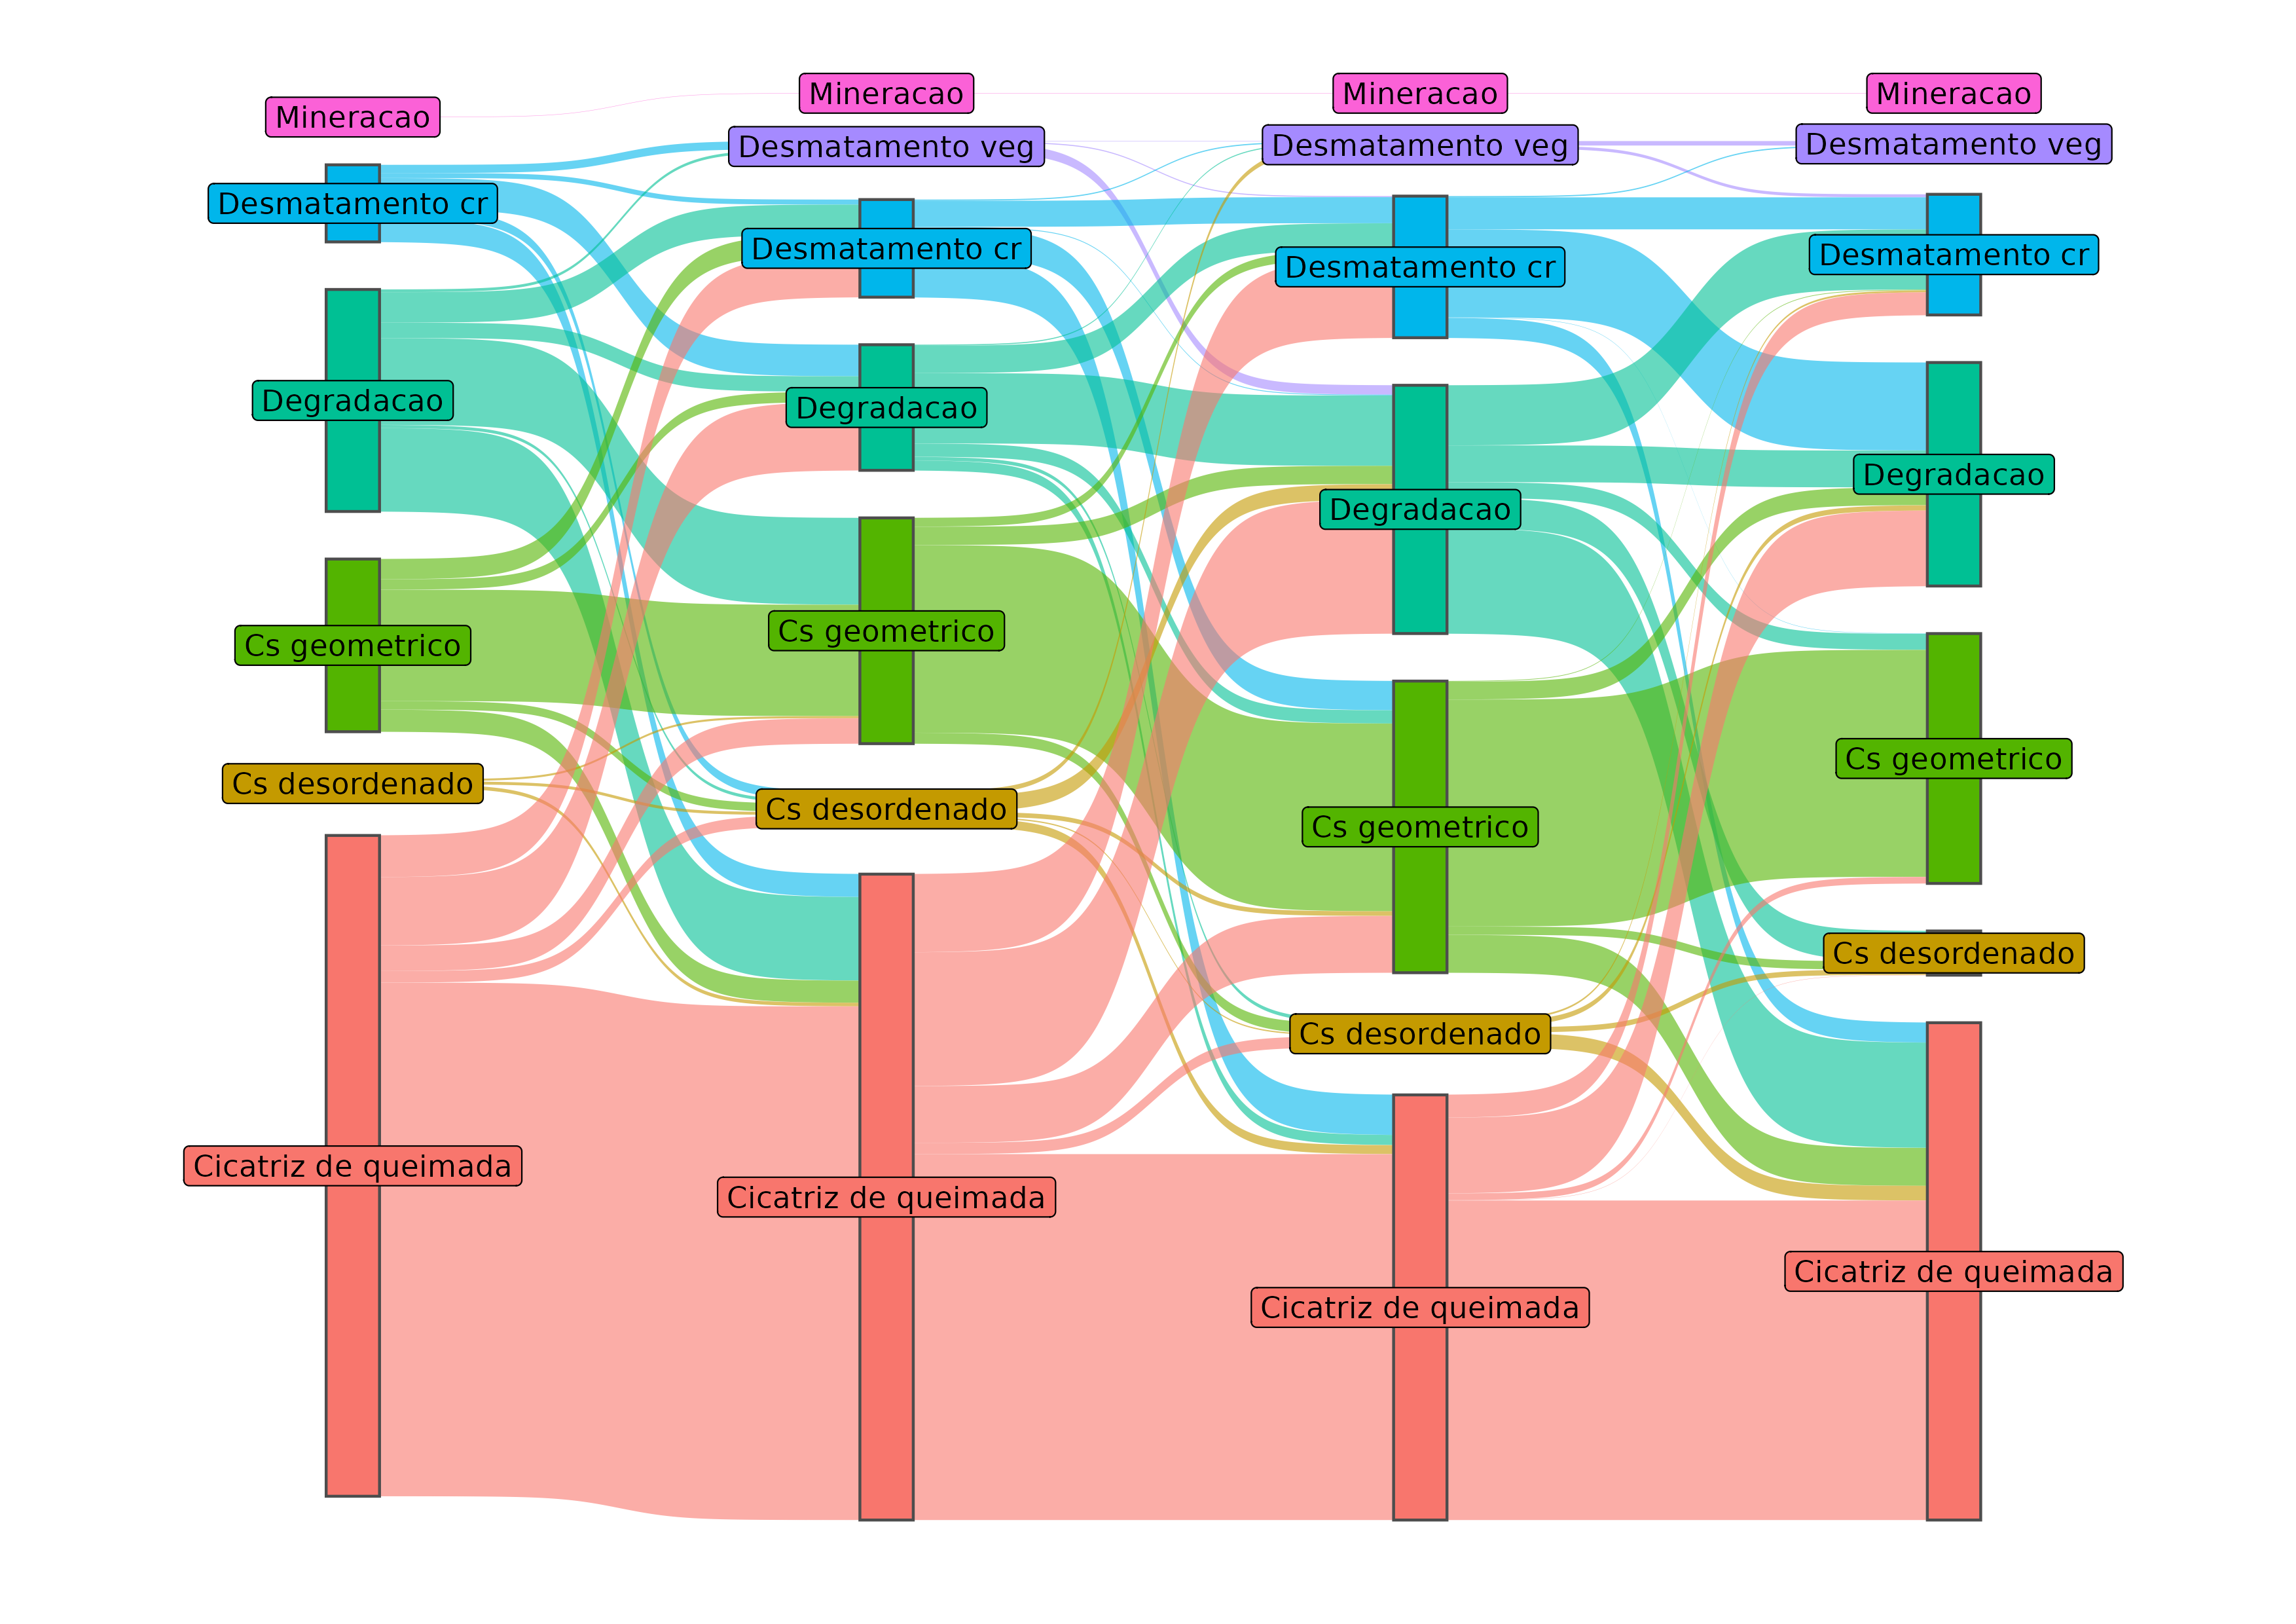
\includegraphics[width=0.75\linewidth]
        {./figures/plot_deter_subarea_trajectory_4.png}
    \end{figure}
\end{frame}

\begin{frame}
    \frametitle{Subarea trajectories (5 warnings)}
    \begin{figure}[h]
        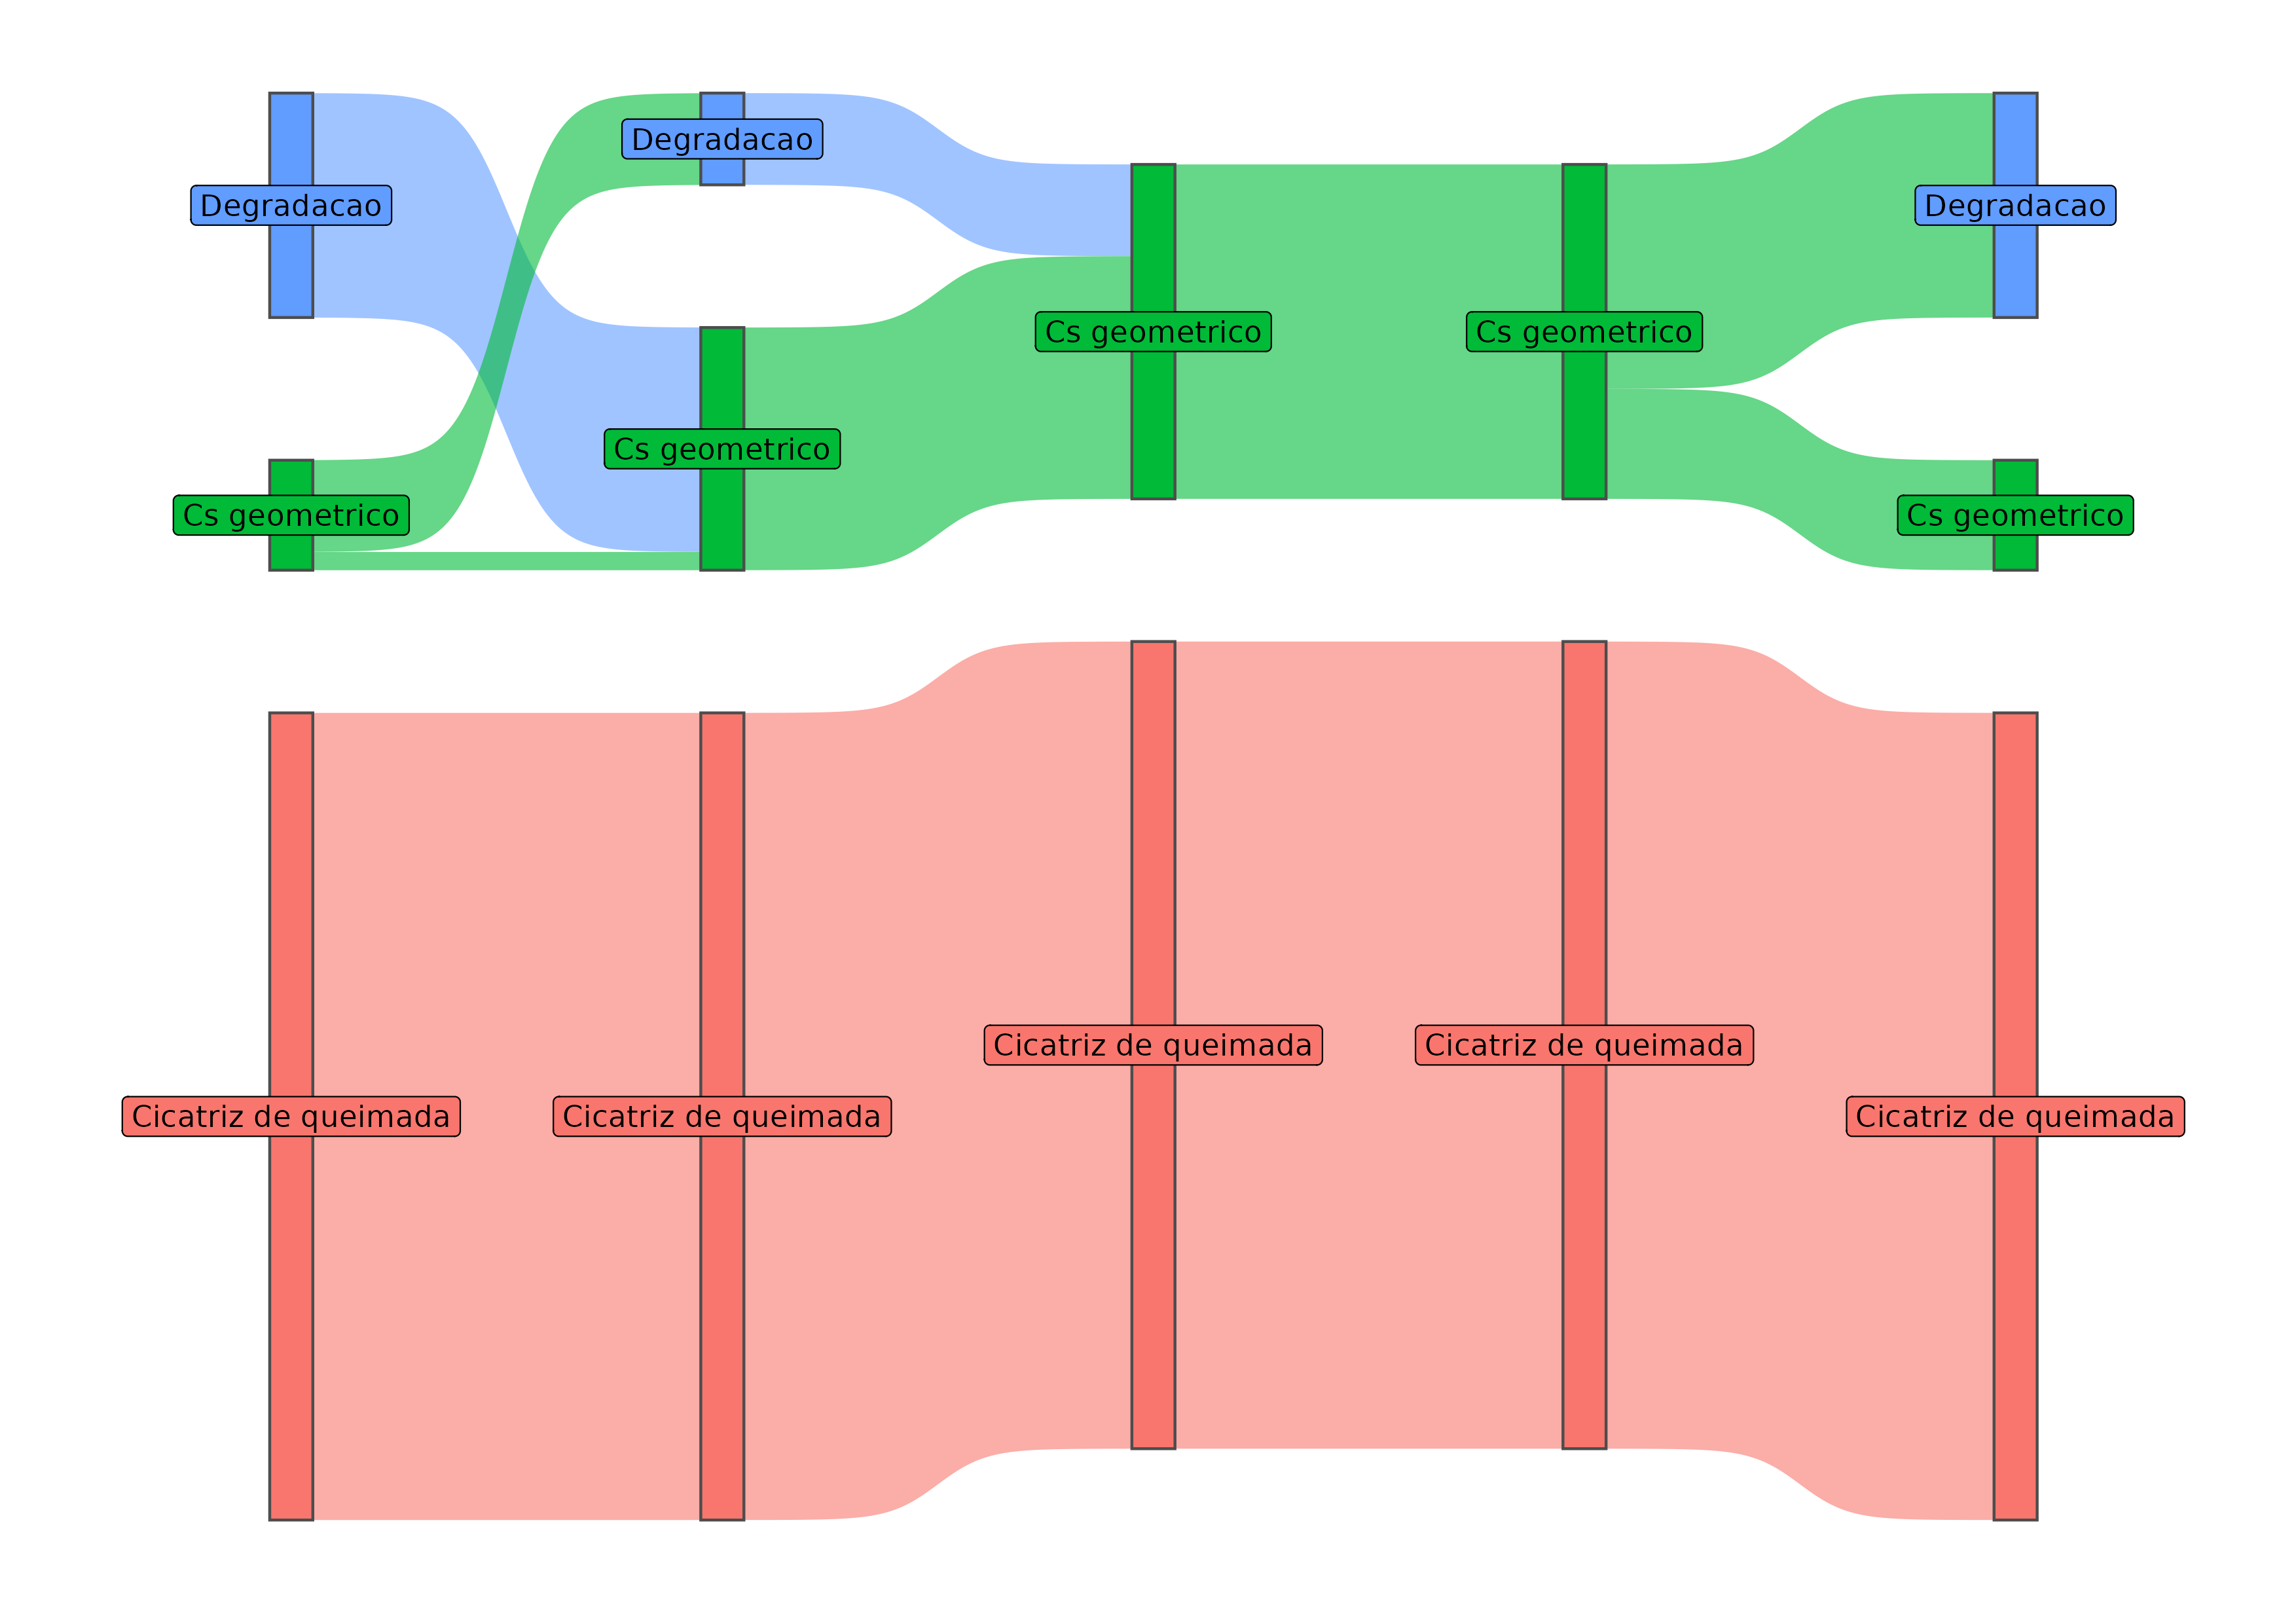
\includegraphics[width=0.75\linewidth]
        {./figures/plot_deter_subarea_trajectory_5.png}
    \end{figure}
\end{frame}

\subsection{Trajectories (including PRODES)}

\begin{frame}
    \frametitle{Subarea trajectories PRODES (2 warnings)}
    \begin{figure}[h]
        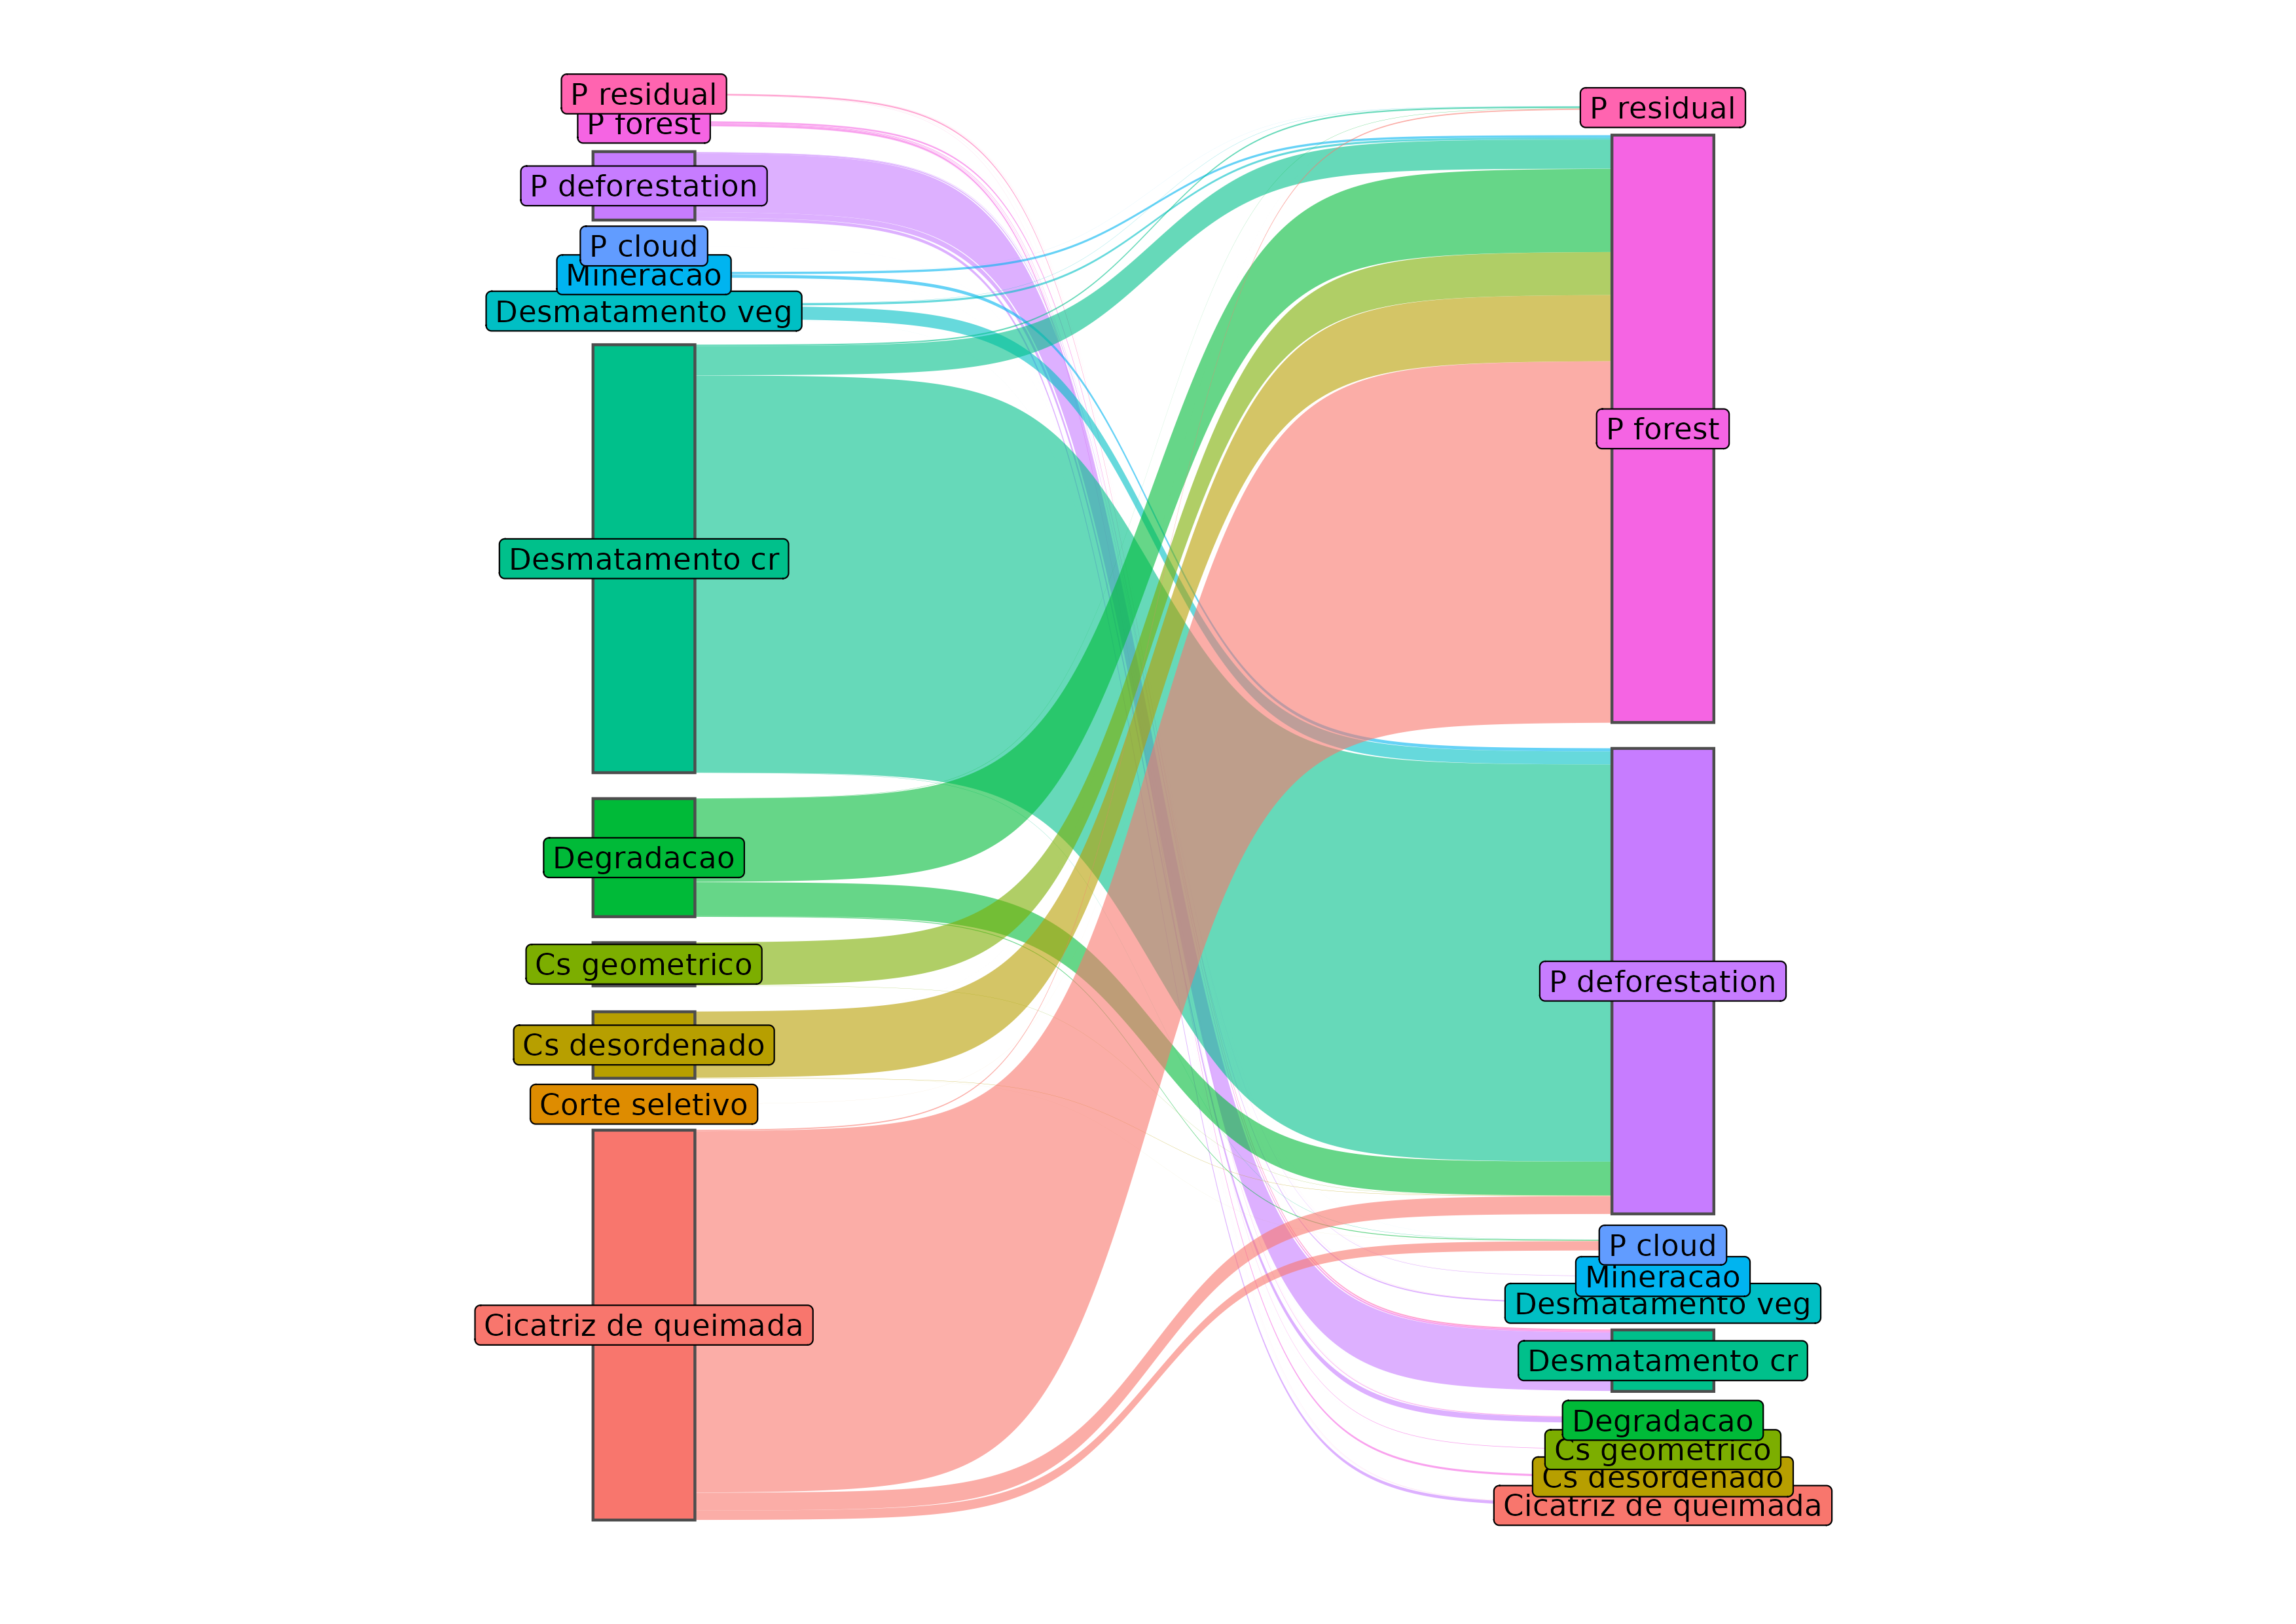
\includegraphics[width=0.75\linewidth]
        {./figures/plot_deter_prodes_subarea_trajectory_2.png}
    \end{figure}
\end{frame}

\begin{frame}
    \frametitle{Subarea trajectories PRODES (3 warnings)}
    \begin{figure}[h]
        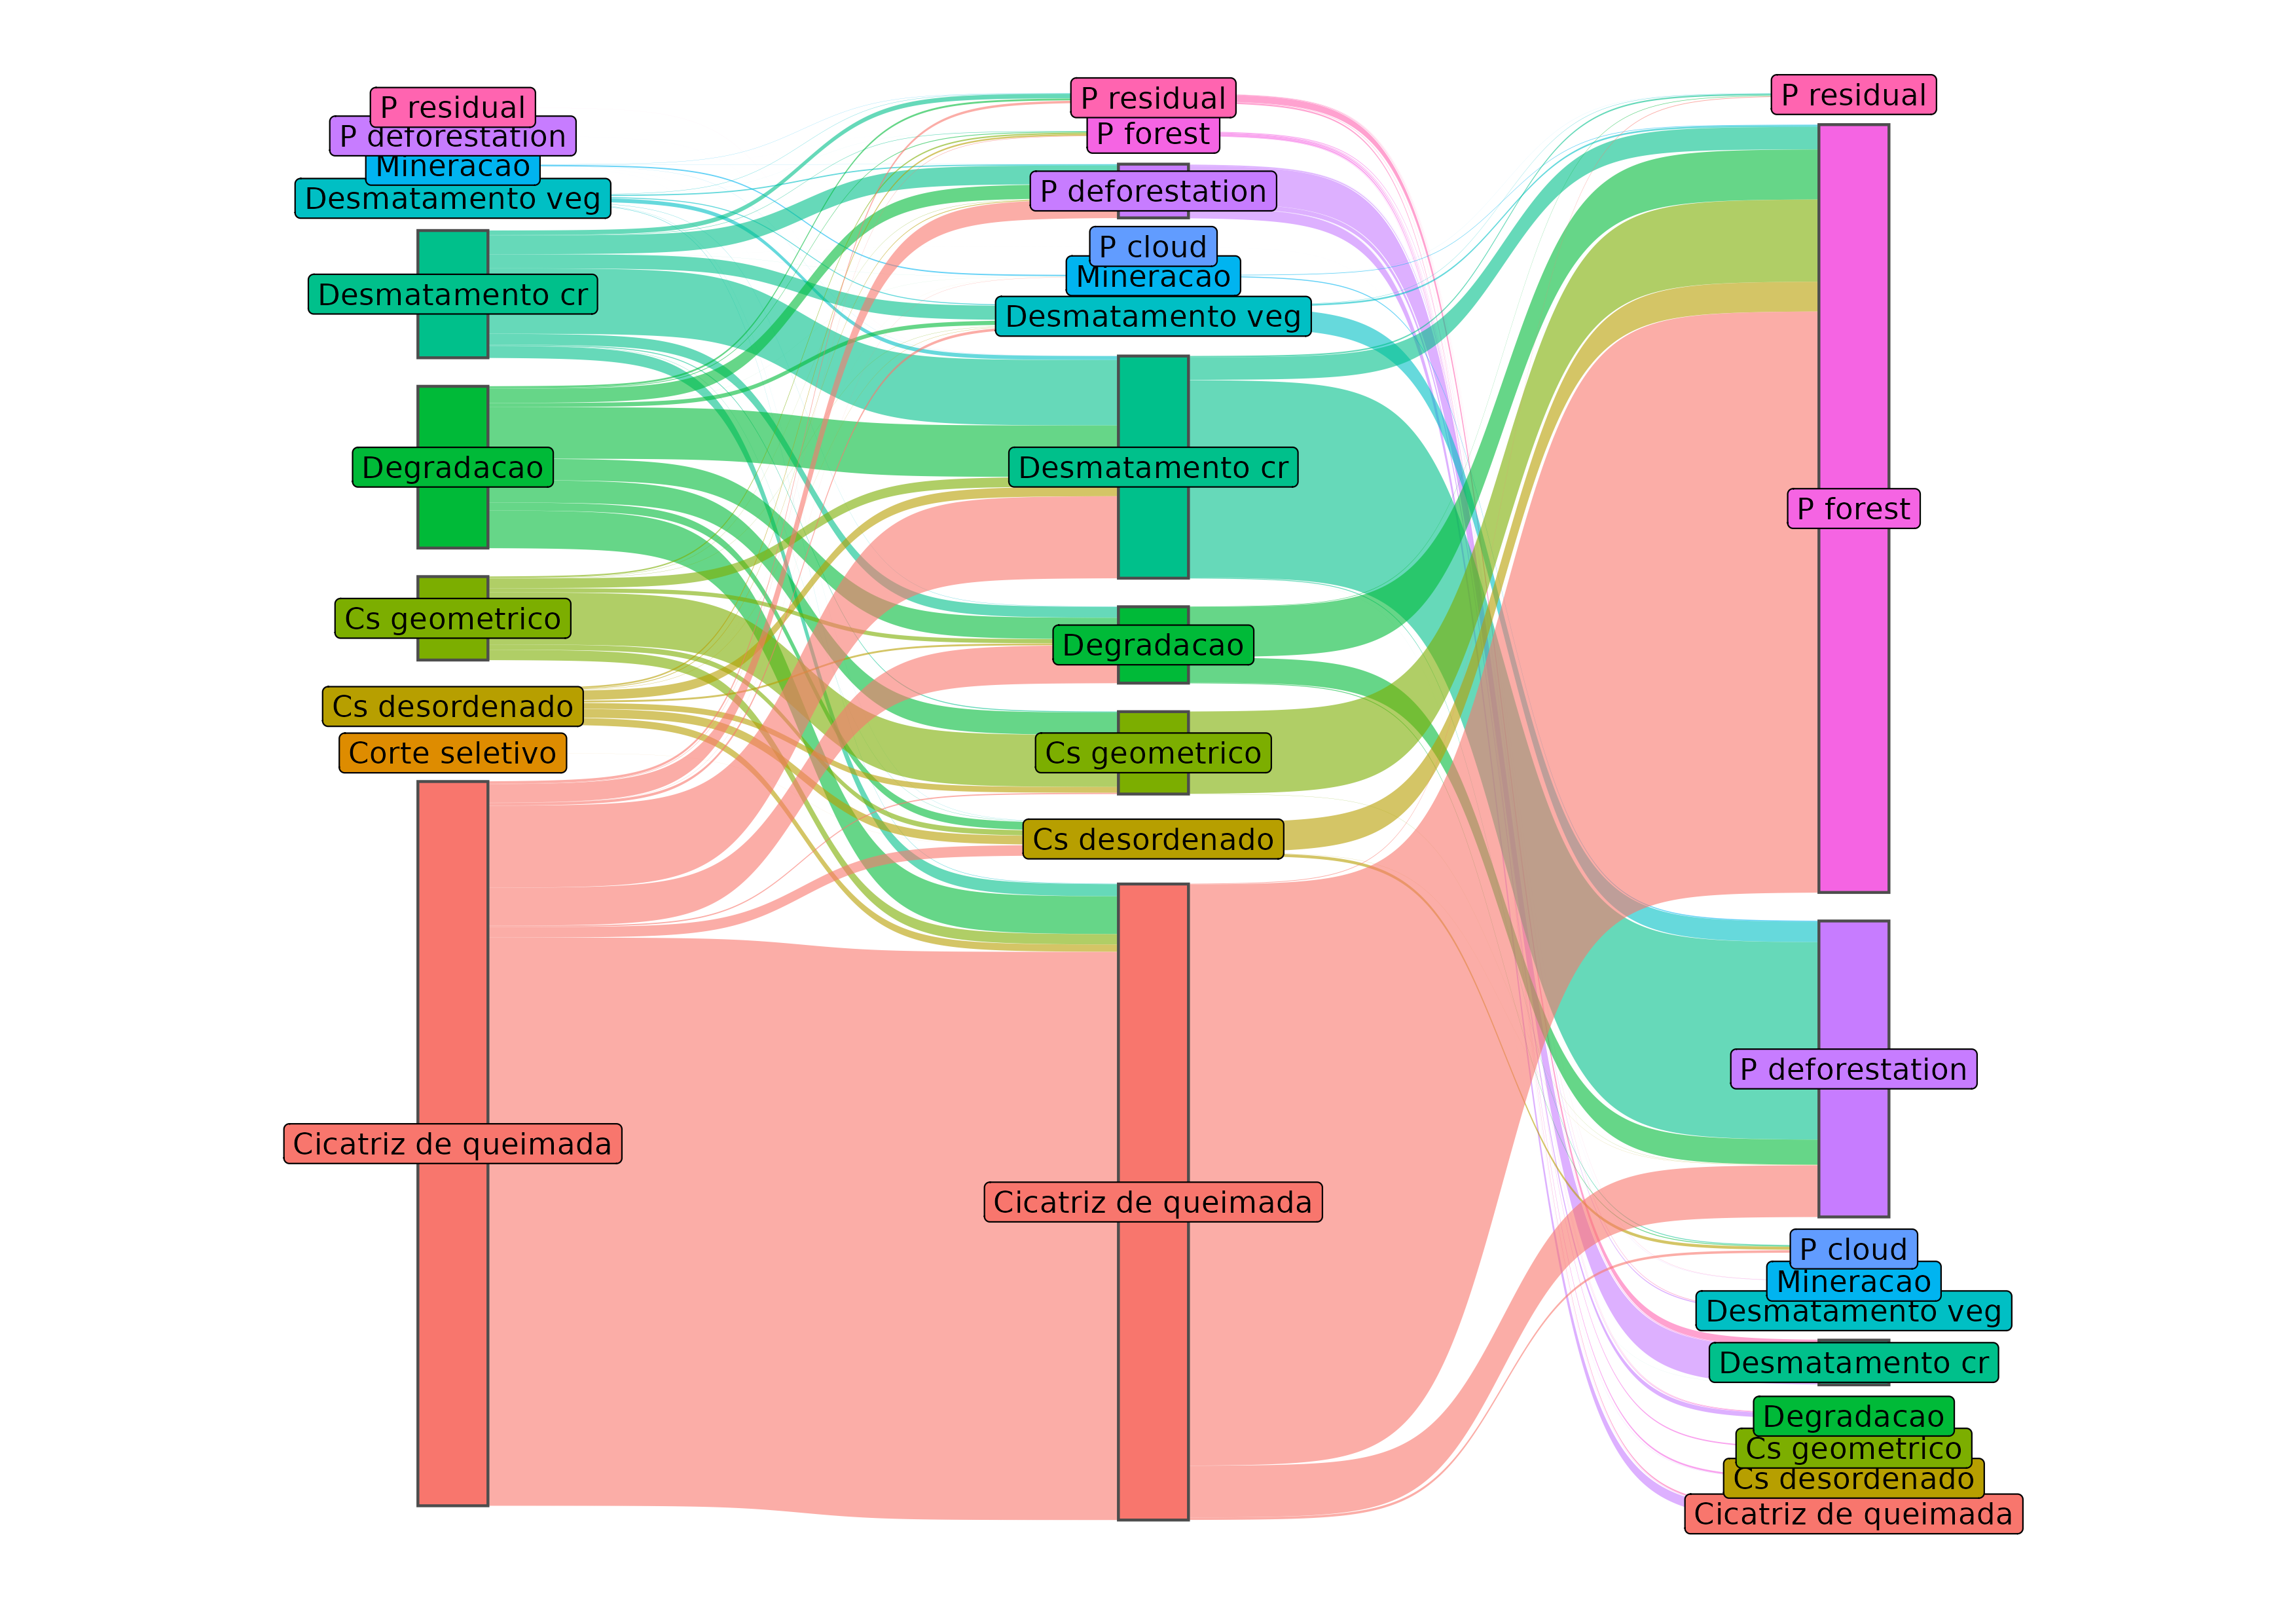
\includegraphics[width=0.75\linewidth]
        {./figures/plot_deter_prodes_subarea_trajectory_3.png}
    \end{figure}
\end{frame}

\begin{frame}
    \frametitle{Subarea trajectories PRODES (4 warnings)}
    \begin{figure}[h]
        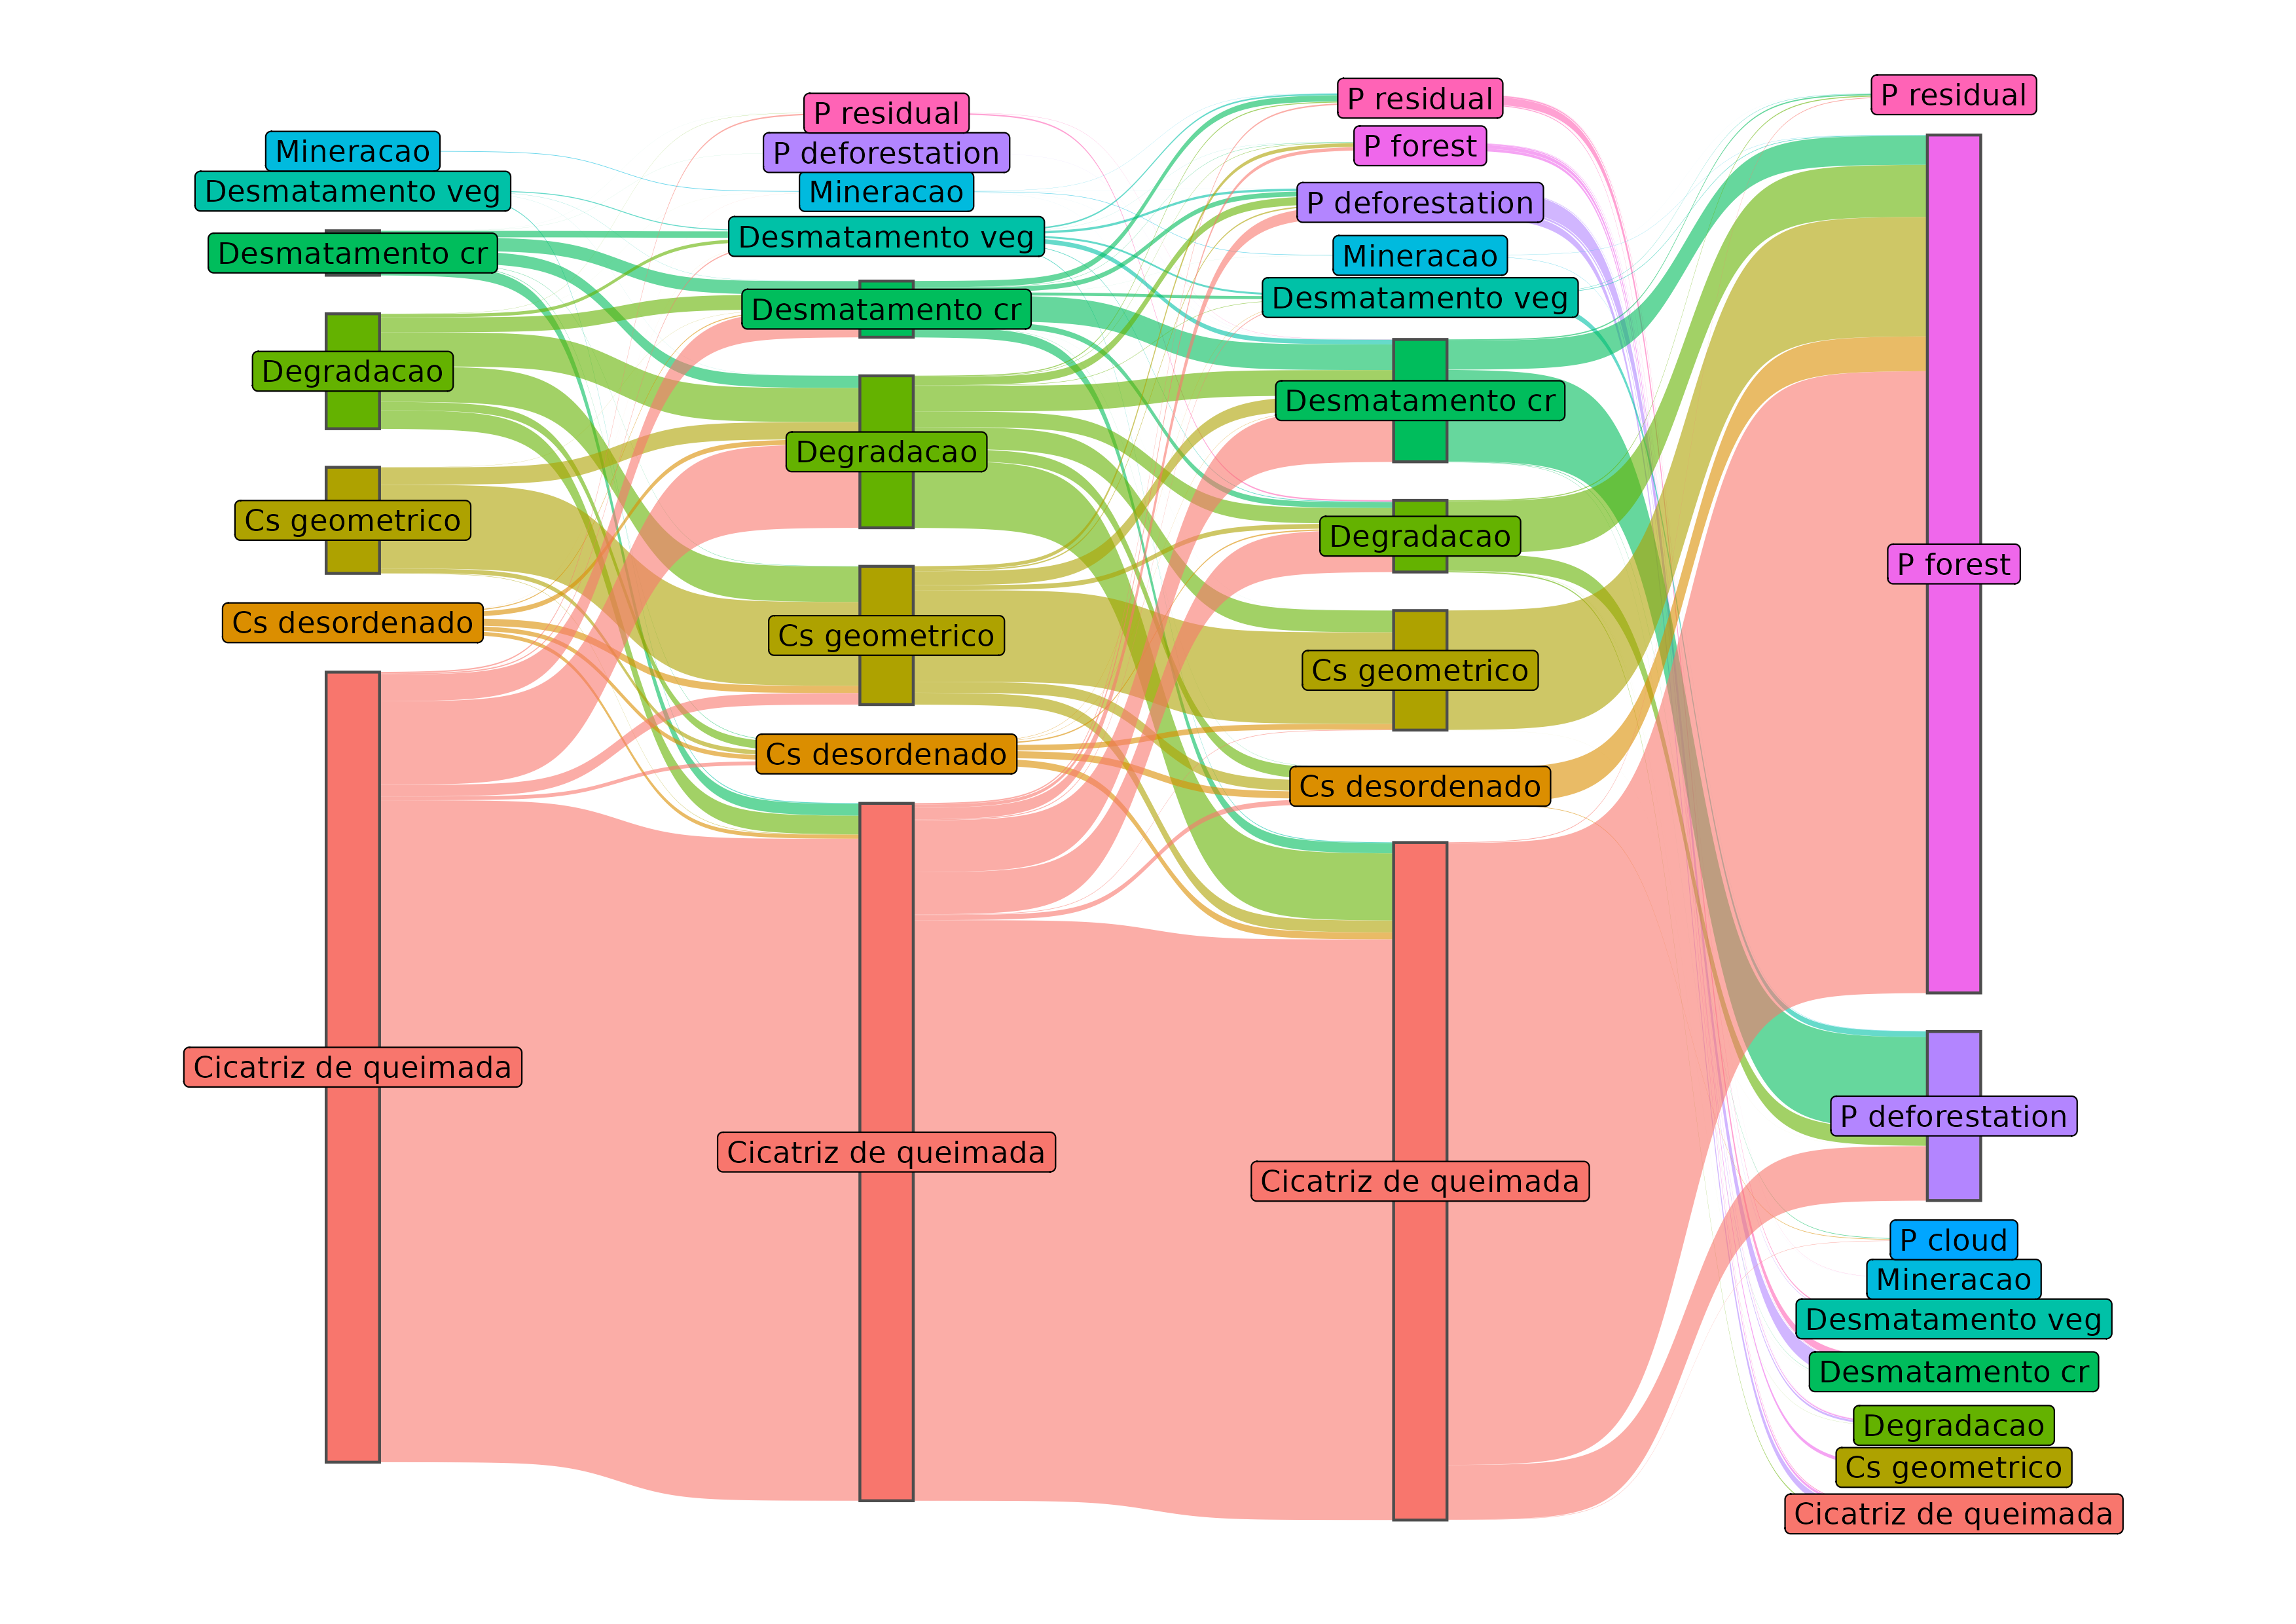
\includegraphics[width=0.75\linewidth]
        {./figures/plot_deter_prodes_subarea_trajectory_4.png}
    \end{figure}
\end{frame}

\begin{frame}
    \frametitle{Subarea trajectories PRODES (5 warnings)}
    \begin{figure}[h]
        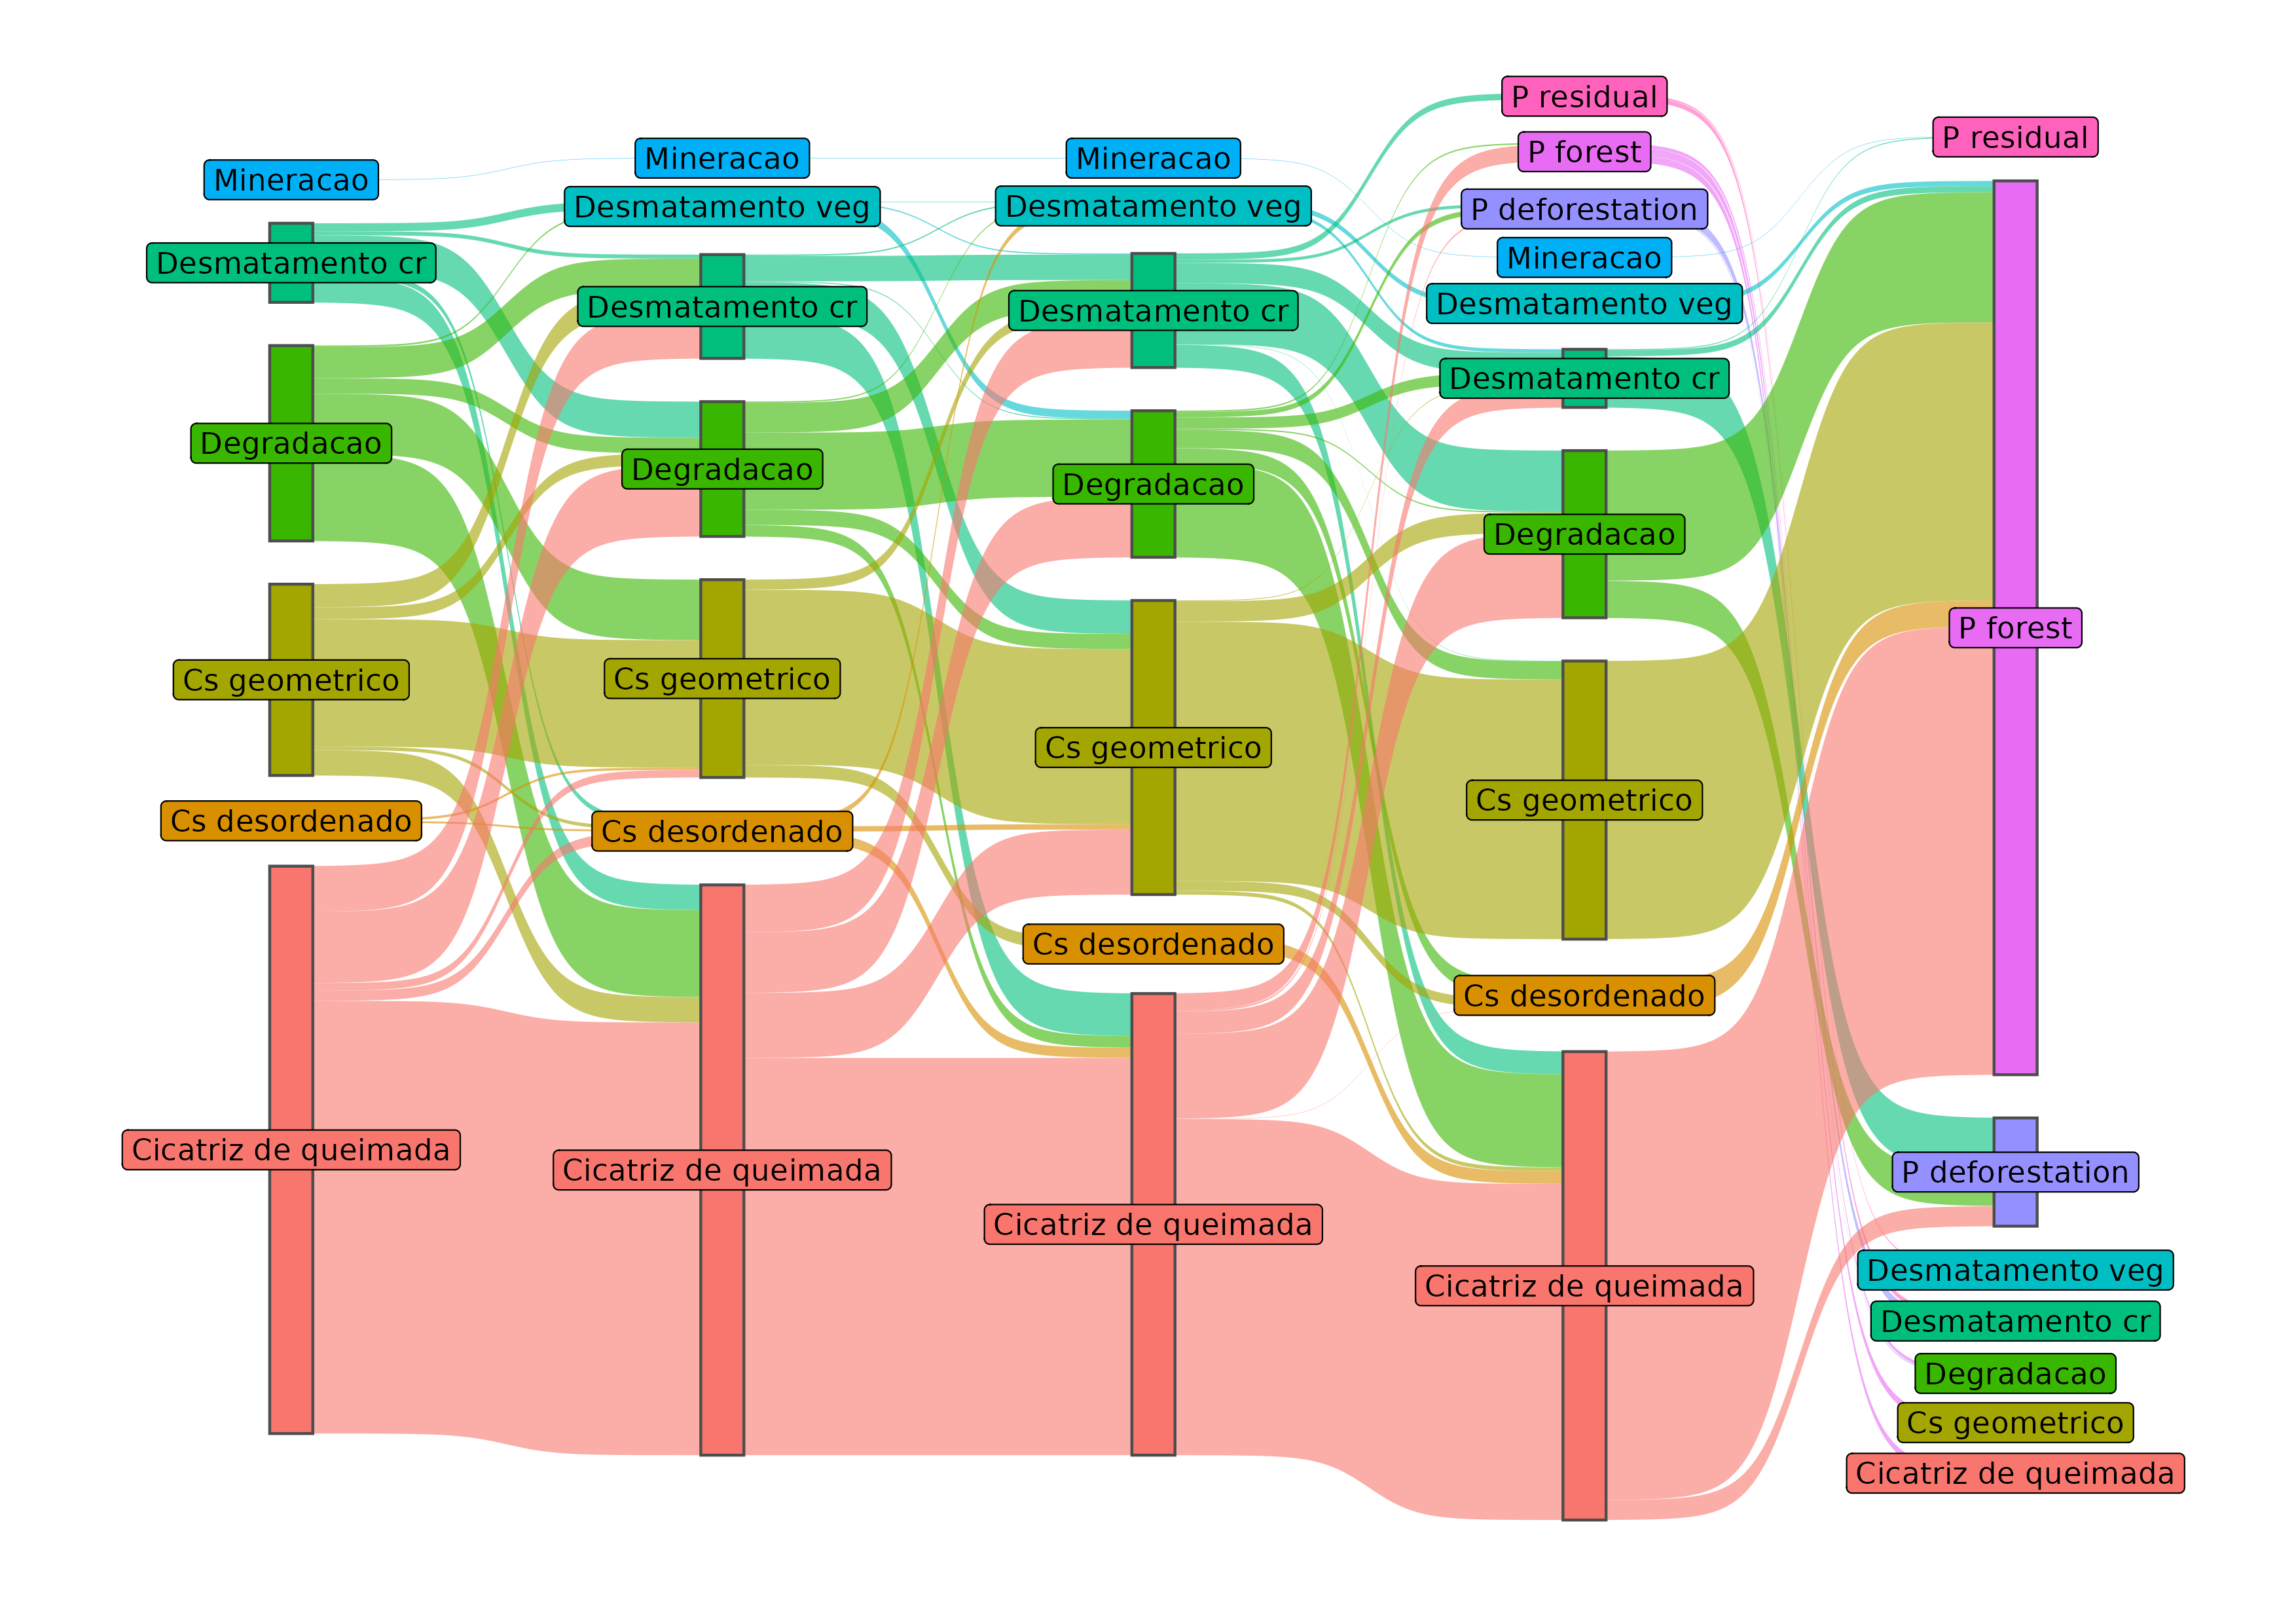
\includegraphics[width=0.75\linewidth]
        {./figures/plot_deter_prodes_subarea_trajectory_5.png}
    \end{figure}
\end{frame}

\begin{frame}
    \frametitle{Subarea trajectories PRODES (6 warnings)}
    \begin{figure}[h]
        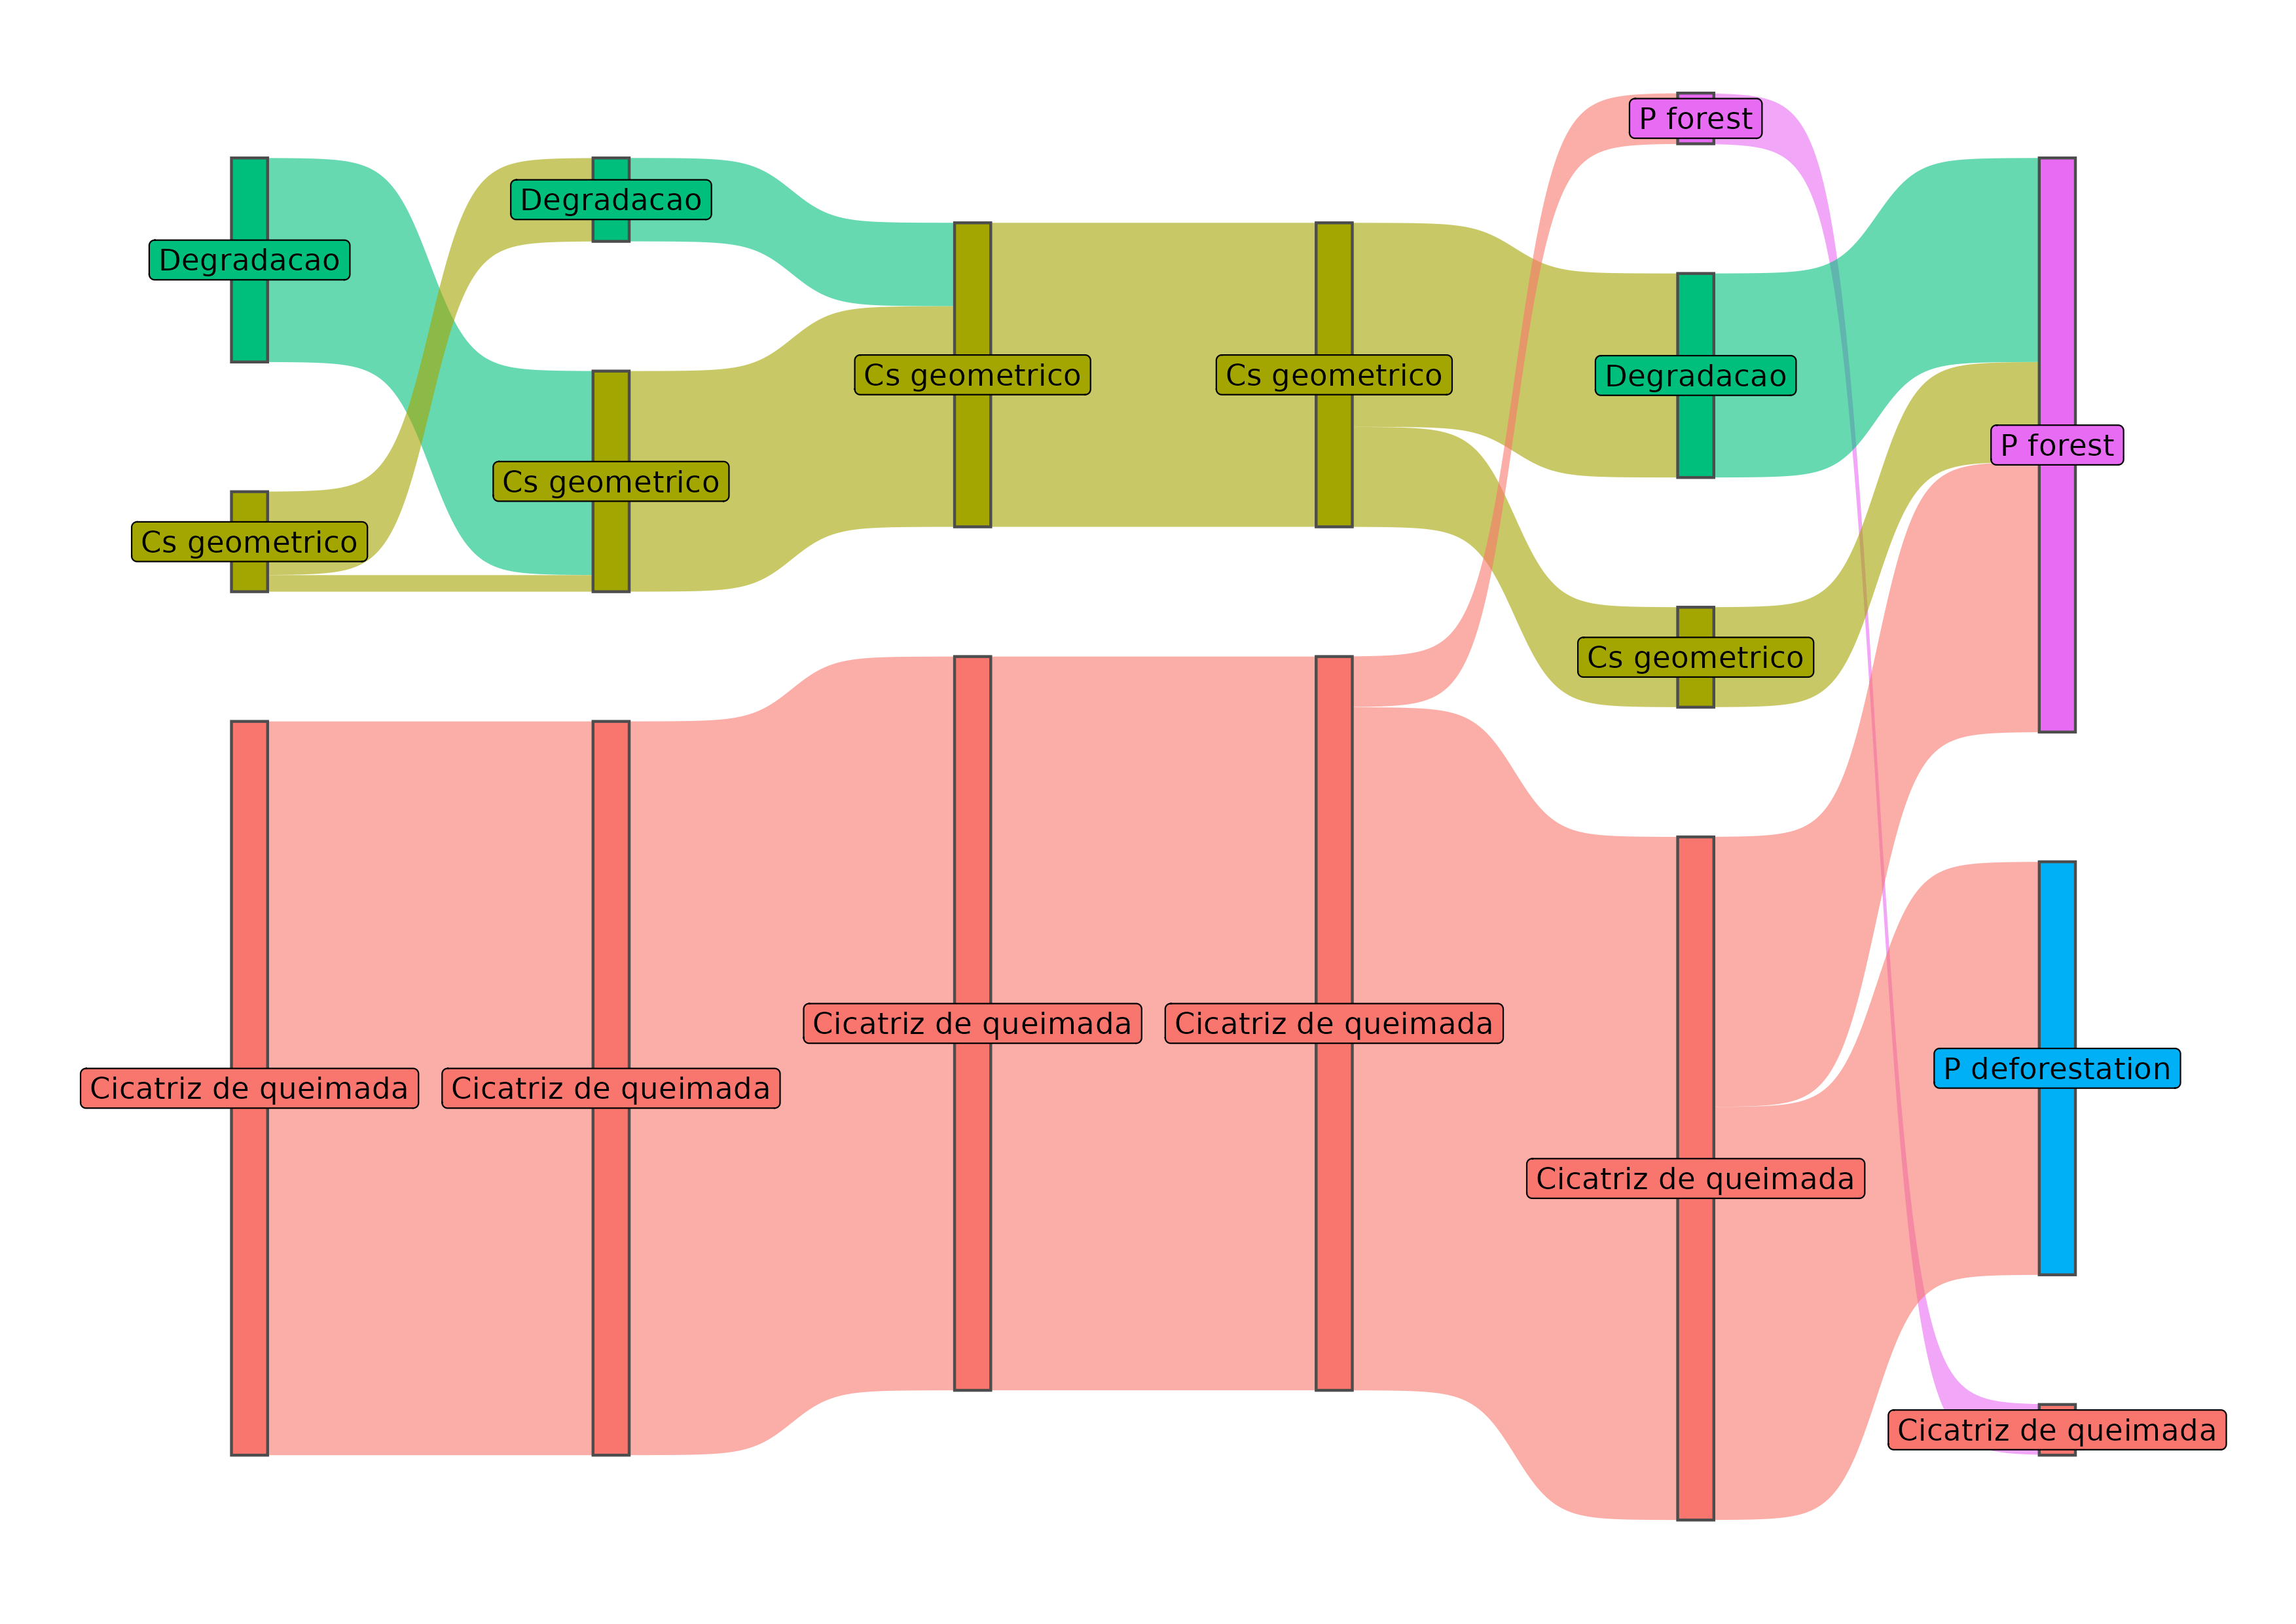
\includegraphics[width=0.75\linewidth]
        {./figures/plot_deter_prodes_subarea_trajectory_6.png}
    \end{figure}
\end{frame}

%
%plot_deter_subarea_trajectory_year.png

%
%plot_fire_spots_by_month.png
%plot_fire_spots_by_month_state.png
%
%an1_plot_deter_prodes_subarea_trajectory_2.png
%an1_plot_deter_prodes_subarea_trajectory_3.png
%an1_plot_deter_prodes_subarea_trajectory_4.png
%an1_plot_deter_prodes_subarea_trajectory_5.png
%an2_plot_deter_prodes_subarea_trajectory_2.png
%an2_plot_deter_prodes_subarea_trajectory_3.png
%an2_plot_deter_prodes_subarea_trajectory_4.png
%an2_plot_deter_prodes_subarea_trajectory_5.png


%%---- 07 ----
%\begin{frame}
%    \frametitle{Number of DETER warnings in SFX}
%    \begin{figure}[h] 
%        \includegraphics[width=0.65\linewidth]
%        {./figures/deter_warnings_size.png}
%        \caption{Note the increasing trend and the small peak in 2018.}
%        \label{fig:deter_warnings_number}
%    \end{figure}
%\end{frame}
%
%%---- 08 ----
%\begin{frame}
%    \frametitle{Periodicity of DETER warnings in SFX}
%    \begin{figure}[h] 
%        \includegraphics[width=0.65\linewidth]
%        {./figures/deter_warnings_size_month.png}
%        \caption{Note Sep-Oct 2018 and Aug-Sep 2020 }
%        \label{fig:deter_warnings_periodicity}
%    \end{figure}
%\end{frame}
%
%%---- 09 ----
%\begin{frame}
%    \frametitle{DETER warnings and time}
%    \begin{itemize}
%        \item The spatial properties of DETER warning areas are inconsistent 
%            along time (shape, size, area, position).
%    \end{itemize}
%\end{frame}
%
%%---- 10 ----
%\begin{frame}
%    \frametitle{Warning subareas are inconsistent along time}
%    \begin{figure}[h] 
%        \includegraphics[width=0.60\linewidth]
%        {./figures/sample_deter_warnings.png}
%        \label{fig:deter_subareas}
%        \caption{Note how DETER warnings overlap differently with time.}
%    \end{figure}
%\end{frame}
%
%%---- 11 ----
%\begin{frame}
%    \frametitle{DETER warnings subareas}
%    \begin{itemize}
%        \item The spatial properties of DETER warning areas are inconsistent 
%            along time (shape, size, area, position).
%        \item DETER subareas maintain their spatial properties along time.
%    \end{itemize}
%\end{frame}
%
%%---- 12 ----
%\begin{frame}
%    \frametitle{DETER warning subareas}
%    \begin{figure}[h] 
%        \includegraphics[width=0.60\linewidth]
%        {./figures/sample_deter_subareas.png}
%        \caption{Note how 3 DETER warnings produce 7 subareas!}
%        \label{fig:deter_subareas}
%    \end{figure}
%\end{frame}
%
%%---- 13 ----
%\begin{frame}
%    \frametitle{Subareas of recurrent warnings}
%    \begin{figure}[h] 
%        \includegraphics[width=0.65\linewidth] 
%        {./figures/plot_area_by_warnings.png}
%        \caption{Most subareas are issued a single warning.}
%        \label{fig:deter_warning_recurrency}
%    \end{figure}
%\end{frame}
%
%%---- 14 ----
%\begin{frame}
%    \frametitle{Days between first and last warnings}
%    \begin{figure}[h] 
%        \includegraphics[width=0.65\linewidth]
%        {./figures/plot_days_first_to_last.png}
%        \caption{The mean lag between 2 and 3 warnings is one year.}
%        % NOTE: Each Box plot shows the median; 
%        %       the first and third quartiles (hinges); 
%        %       1.5 times the inter-quartile range from the hinges; 
%        %       and the outliers.
%        \label{fig:deter_warning_first_to_last}
%    \end{figure}
%\end{frame}
%
%%---- 15 ----
%\begin{frame}
%    \frametitle{Reproducibility - DETER processing}
%    \begin{figure}[h] 
%        \includegraphics[width=0.95\linewidth] 
%        {./figures/deter_processing.png}
%        \caption{DETER data preprocessiing before analysis.}
%        \label{fig:deter_processing}
%    \end{figure}
%\end{frame}
%

\section{Final remarks}

\begin{frame}
    \frametitle{Final remarks}
    \begin{itemize}
        \item The analysis of DETER warning subareas along time could improve 
            the characterization of forest degradation.
        \item Potential applications of our work are:
            \begin{itemize}
                \item Improve estimation of emissions of greenhouse gases, i.e.
                    our data could help avoiding double counting.
                \item Identify spatio-temporal areas which could help training 
                    Machine-Learning algorithms for automatic identification 
                    of forest degradation.
            \end{itemize}
        \item Code available at 
            \url{https://github.com/albhasan/treesburnareas}
        \item This is a follow-up of the work presented at the XX Brazilian
            Symposium on Remote Sensing~\cite{sanchez2023}.
    \end{itemize}
\end{frame}

\begin{frame}[allowframebreaks]
    \frametitle{References}
    \bibliographystyle{amsalpha}
    \bibliography{pg_sere_2024.bib}
\end{frame}

\end{document}
